%\documentclass[first,firstsupp,handout,compress,notes,navigation,hyperref,table]{ETHclass}
%\documentclass[first,firstsupp,handout,lastsupp]{ETHclass}
\documentclass[first,firstsupp,lastsupp,last,hyperref,table]{ETHclass}
%\documentclass[first,firstsupp]{ETHclass}
\usepackage{etex}


\usepackage{adjustbox}
\usepackage{amsmath}
\usepackage{amssymb}
\usepackage{animate}
\usepackage{booktabs}
\usepackage{charter}
\usepackage{enumitem}
\usepackage{etoolbox}
\usepackage{ifthen}
\usepackage{longtable}
\usepackage{mathrsfs}
\usepackage{multicol}
\usepackage{nicefrac}
\usepackage{pgf}
\usepackage{pgfpages}
\usepackage{pgfplots}
\usepackage{pifont}
\usepackage{ragged2e}
\usepackage{standalone}
\usepackage[caption=false]{subfig}
\usepackage{tabularx}
\usepackage{tikz}
\usepackage{verbatim}
\usepackage{wasysym}
\usepackage{xcolor}
\usepackage{hyperref}

\pgfplotsset{compat=1.7}

\setbeamertemplate{navigation symbols}{}
\usetikzlibrary{arrows,decorations.pathreplacing,positioning,shapes,shadows}

%\usepackage[style=numeric-comp]{biblatex}

%\usepackage{lipsum}

%\usetikzlibrary{fit}
\usetikzlibrary{arrows}
\usetikzlibrary{trees}

% Options for beamer:
%
% 9,10,11,12,13,14,17pt  Fontsizes
%
% compress: navigation bar becomes smaller
% t       : place contents of frames on top (alternative: b,c)
% handout : handoutversion
% notes   : show notes
% notes=onlyslideswithnotes
%
%hyperref={bookmarksopen,bookmarksnumbered} : Needed for menues in
%                                             acrobat. Also need
%                                             pdftex as option or
%                                             compile with
% pdflatex '\PassOptionsToPackage{pdftex,bookmarksopen,bookmarksnumbered}{hyperref} \input{file}'

%\usepackage{beamerseminar}
%\usepackage[accumulated]{beamerseminar}
                                % remove ``accumulated'' option
                                % for original behaviour
%\usepackage{beamerbasenotes}
%\setbeamertemplate{note page}[plain]
%\setbeameroption{notes on second screen}

%\setbeamertemplate{note page}[plain]
%\setbeamertemplate{note page}{\ \\[.3cm]
%\textbf{\color{blue}Notes:}\\%[0.1cm]
%{\footnotesize %\tiny
%\insertnote}}
%\setbeameroption{notes on second screen}


\setbeamertemplate{navigation symbols}{} % suppresses all navigation symbols:
% \setbeamertemplate{navigation symbols}[horizontal] % Organizes the navigation symbols horizontally.
 %\setbeamertemplate{navigation symbols}[vertical] % Organizes the navigation symbols vertically.
% \setbeamertemplate{navigation symbols}[only frame symbol] % Shows only the navigational symbol for navigating frames.

\setlayoutscale{0.5}
\setparametertextfont{\scriptsize}
\setlabelfont{\scriptsize}

% \useoutertheme[subsection=false]{miniframes}
% \usepackage{etoolbox}
% \makeatletter
% \patchcmd{\slideentry}{\advance\beamer@xpos by1\relax}{}{}{}
% \def\beamer@subsectionentry#1#2#3#4#5{\advance\beamer@xpos by1\relax}%
% \makeatother

% \makeatletter
%     \newenvironment{withoutheadline}{
%        \setbeamertemplate{headline}{%
% \vspace{15pt}
% }
%     }{}
% \makeatother

\makeatletter
    \newenvironment{withoutheadline}{
         \setbeamertemplate{headline}{%
\vspace{35pt}
}
        %\def\beamer@entrycode{\vspace*{-1.5\headheight}}
    }{}
\makeatother

\makeatletter
    \newenvironment{tocframe}{
         \setbeamertemplate{headline}{%
\vspace{35pt}
}
         \setbeamertemplate{footline}{%
\leavevmode%
  \hbox{
    \begin{beamercolorbox}[wd=.3\paperwidth,ht=2.5ex,dp=0.75ex,left]{author in head/foot}%
      \qquad\color{white}{\tiny\underline{Luca Di Stasio}}%
    \end{beamercolorbox}%

    \begin{beamercolorbox}[wd=.45\paperwidth,ht=2.5ex,dp=0.75ex,center]{title in head/foot}%
      \color{white}{Lule\aa\ (SE) - December 13, 2019}%
    \end{beamercolorbox}%

    \begin{beamercolorbox}[wd=.2\paperwidth,ht=2.5ex,dp=0.75ex,right]{title in head/foot}%
      \color{white}{\insertframenumber\totalframes}%
    \end{beamercolorbox}%
  }
}
        %\def\beamer@entrycode{\vspace*{-1.5\headheight}}
    }{}
\makeatother

\newcommand{\Cross}{$\mathbin{\tikz [x=1.4ex,y=1.4ex,line width=.2ex, red] \draw (0,0) -- (1,1) (0,1) -- (1,0);}$}%

\newcommand{\Checkmark}{$\color{green}\mathbf{\checkmark}$}

\setbeamerfont{subsection in toc}{size=\tiny}

\makeatletter
\patchcmd{\beamer@sectionintoc}
  {\vfill}
  {\vskip1.5\itemsep}
  {}
  {}
\makeatother

\setbeamertemplate{frametitle continuation}{}

\setbeamertemplate{bibliography entry title}{}
\setbeamertemplate{bibliography entry author}{}
\setbeamertemplate{bibliography entry location}{}
\setbeamertemplate{bibliography entry note}{}

\setbeamercolor*{bibliography entry title}{fg=black}
\setbeamercolor*{bibliography entry author}{fg=black}
\setbeamercolor*{bibliography entry location}{fg=black}
\setbeamercolor*{bibliography entry note}{fg=black}
% and kill the abominable icon
%\setbeamertemplate{bibliography item}{\color{forestgreen}$\blacktriangleright$}
\setbeamertemplate{bibliography item}{\insertbiblabel}
%\setbeamertemplate{bibliography item}{\theenumiv}

\newcommand{\highlightred}[1]{%
  \colorbox{red!50}{$\displaystyle#1$}}

\newcommand{\highlightyellow}[1]{%
  \colorbox{yellow!50}{$\displaystyle#1$}}

\newcommand{\highlightgreen}[1]{%
  \colorbox{green!50}{$\displaystyle#1$}}

\AtBeginSection[]{
  \begin{frame}
  \vfill
  \centering
  \begin{beamercolorbox}[sep=8pt,center,shadow=true,rounded=true]{title}
    \usebeamerfont{frametitle}
\includegraphics[width=2ex]{freccia_trasparente_verde_foresta.png}\hspace{.5ex}~{\LARGE \textsc{\bfseries \insertsectionhead}}\par%
  \end{beamercolorbox}
  \vfill
  \end{frame}
}

\hyphenpenalty=5000
\tolerance=1000

\graphicspath{{figures/}}

\newenvironment{system}{\left\lbrace\begin{array}{@{}l@{}}}{\end{array}\right.}

\newenvironment{subsystem}{\left\lgroup\begin{array}{@{}l@{}}}{\end{array}\right.}

\defbeamertemplate*{title page}{customized}[1][]
{
\usebeamerfont{subtitle}
\usebeamercolor[fg]{subtitle}

\vspace{-2cm}

{\flushleft
 \usebeamerfont{title}{\inserttitle}\par
}

%\vspace{-.5cm}
%\vspace{-.25cm}
{\flushright
\setbeamercolor{author}{bg=white,fg=Red}
\usebeamerfont{author}{\footnotesize \insertauthor} \par}

\vspace{-.25cm}

{\flushright
\usebeamerfont{institute}{\tiny \insertinstitute}\par }

\vspace{0.5cm}

{\centering
\usebeamerfont{date}{\scriptsize \insertdate} \par }


}


\begin{document}
\setbeamertemplate{caption}{\raggedright\insertcaption\par}

\title{\textsc{\small \textbf{Influence of microstructure on debonding at the fiber/matrix interface in fiber-reinforced polymers under tensile loading}}}
\author{\vspace*{-0.3cm}\textbf{Luca Di Stasio}$^{1,2}$\\[3.5pt]{\scriptsize \textbf{Supervisors}: Janis Varna$^{1}$, Zoubir Ayadi$^{2}$}}
%\institute{ Science et Ing\'enierie des Mat\'eriaux et M\'etallurgie (SI2M), Institut Jean Lamour, Nancy, France\\Department of Engineering Sciences and Mathematics, Division of Materials Science, Lule\aa\ University of Technology, Lule\aa, Sweden}
\institute{$^{1}$Division of Materials Science, Lule\aa\ University of Technology, Lule\aa, Sweden\\$^{2}$EEIGM \& IJL, Universit\'e de Lorraine, Nancy, France}
\date{\vspace*{-0.275cm}\scriptsize Lule\aa\ (SE) - December 13, 2019}

\begin{frame}[plain]
    \titlepage

\end{frame}

\begin{tocframe}
\begin{frame}
\frametitle{\vspace*{0.25cm}Outline}
\justifying
\vspace*{-0.5cm}
% \tableofcontents[hidesubsections]
% \begin{multicols}{2}
% \tableofcontents[hidesubsections]
% \end{multicols}
% \begin{columns}[t]
%         \begin{column}{.5\textwidth}
%             \tableofcontents[sections={1-2}]
%         \end{column}
%         \begin{column}{.5\textwidth}
%             \tableofcontents[sections={3-6}]
%         \end{column}
%     \end{columns}
% \end{frame}
\tableofcontents[hidesubsections]
\end{frame}
\end{tocframe}

%\note{}

%\begin{frame}
%\pagediagram
%\end{frame}
%% \note{}

%\section[Transverse Cracking in FRPCs]{Initiation of Transverse Cracking in Fiber Reinforced Polymer Composites (FRPCs): Microscopic Observations \& Modeling}

\section{Introduction}

\subsection{Challenges of the transport sector}

\begin{frame}
\frametitle{Challenges of the transport sector}
\vspace{-0.5cm}
\centering
\begin{itemize}[label=\ding{212}]
\item Institutional and popular pressure to reduce $CO_{2}$ emissions
\end{itemize}
\begin{columns}[c]
\begin{column}{0.5\textwidth}
\centering
\begin{figure}
\centering
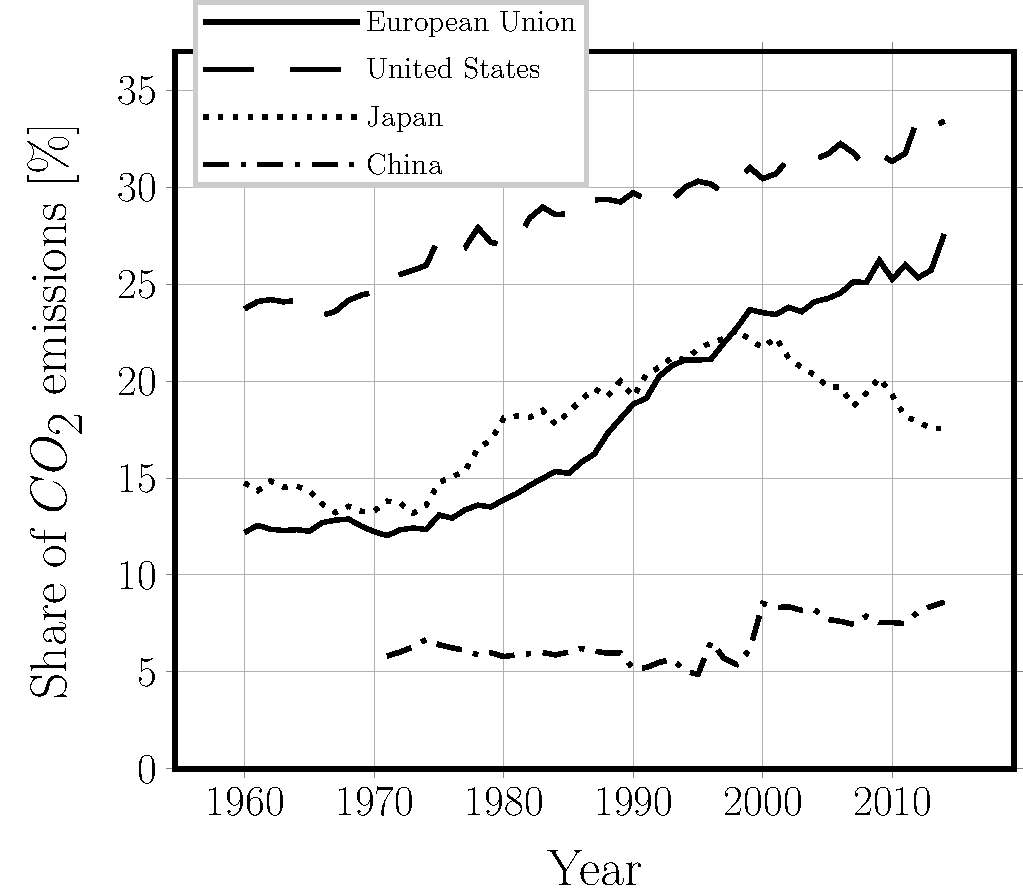
\includegraphics[width=\columnwidth]{co2transportshare.pdf}
\end{figure}
\end{column}
\begin{column}{0.5\textwidth}
\centering
\begin{figure}
\centering
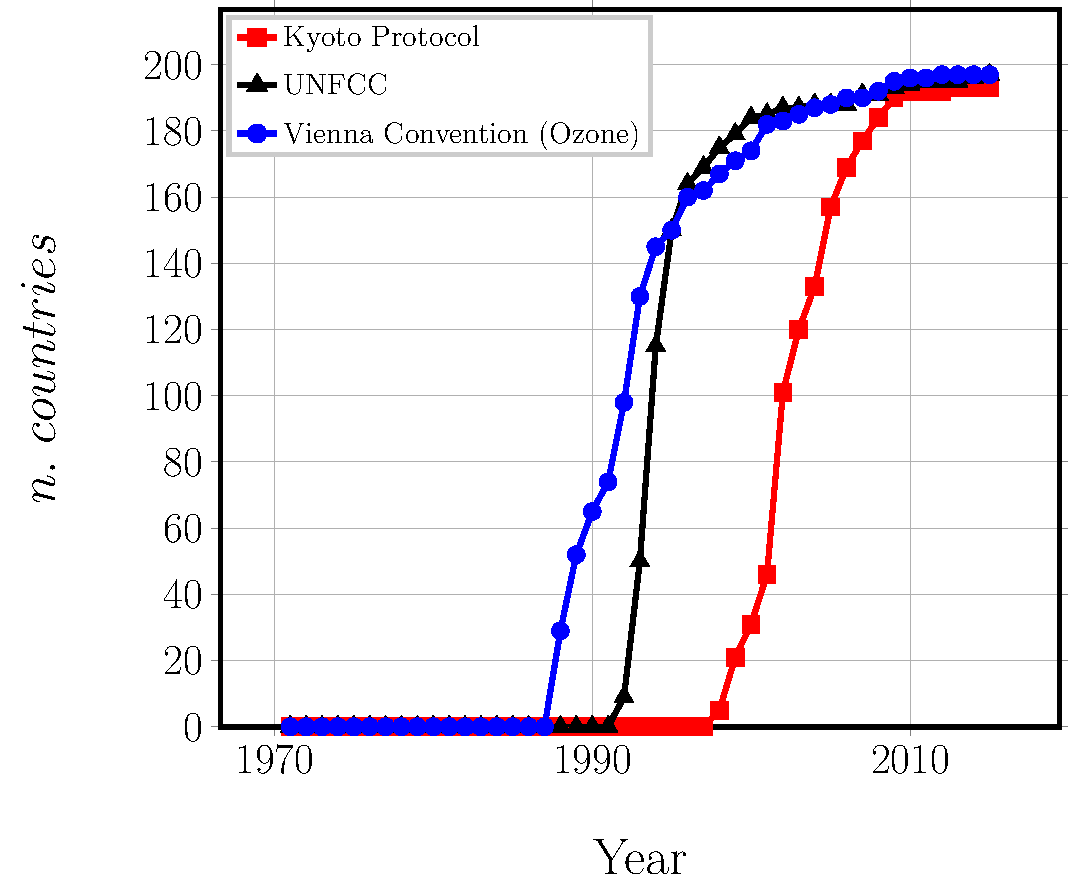
\includegraphics[width=\columnwidth]{climate-deals-signataries.pdf}
\end{figure}
\end{column}
\end{columns}
\end{frame}

\addtocounter{framenumber}{-1}

\begin{frame}
\frametitle{Challenges of the transport sector}
\vspace{-0.5cm}
\centering
\begin{itemize}[label=\ding{212}]
\item Downward pressure on prices
\end{itemize}
\begin{columns}[c]
\begin{column}{0.55\textwidth}
\centering
\begin{figure}
\centering
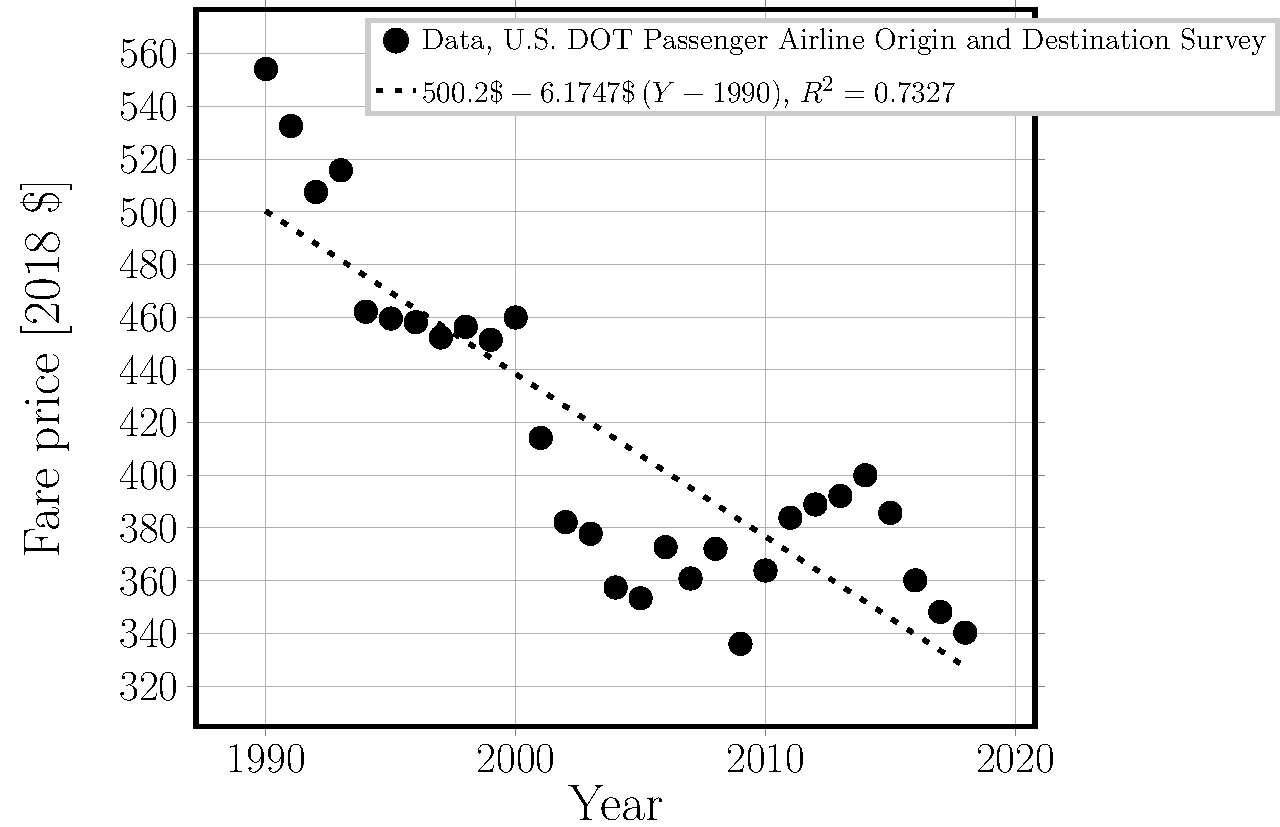
\includegraphics[width=\columnwidth]{airlinefarecost.pdf}
\end{figure}
\end{column}
\begin{column}{0.45\textwidth}
\centering
\begin{figure}
\centering
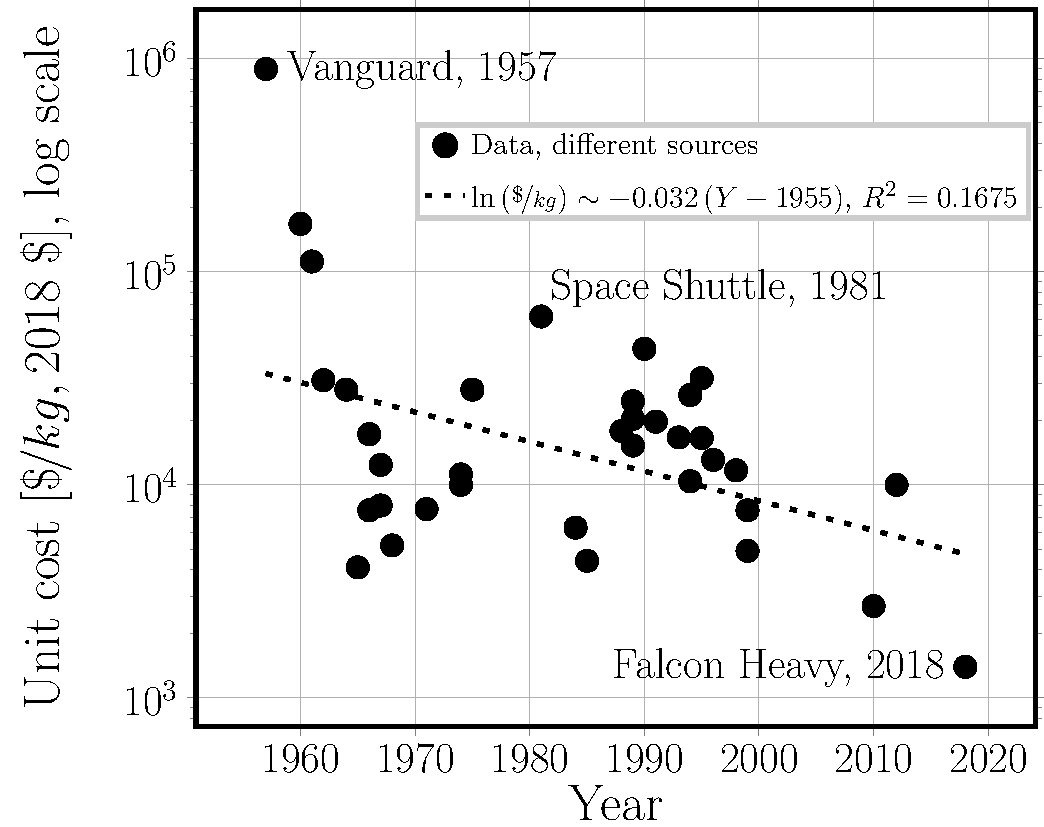
\includegraphics[width=\columnwidth]{spacetravelcost.pdf}
\end{figure}
\end{column}
\end{columns}
\end{frame}

\addtocounter{framenumber}{-1}

\begin{frame}
\frametitle{Challenges of the transport sector}
\vspace{-0.25cm}
\centering
\begin{itemize}[label=\ding{212}]
\item Strict requirements of safety and crashworthiness
\end{itemize}
\vspace{-0.2cm}
\begin{columns}[c]
\begin{column}{0.5\textwidth}
\centering
\begin{figure}
\centering
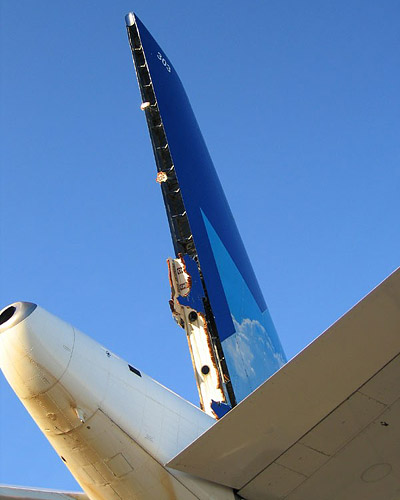
\includegraphics[width=0.8\columnwidth]{A310-308.jpg}
\end{figure}
\end{column}
\begin{column}{0.5\textwidth}
\centering
\begin{figure}
\centering
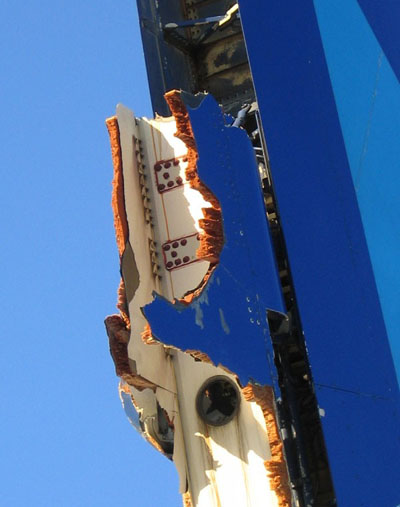
\includegraphics[width=0.8\columnwidth]{A310-308-detail.jpg}
\end{figure}
\end{column}
\end{columns}
\end{frame}

\subsection{The Thin-ply ``Advantage''}

\begin{frame}
\frametitle{\vspace{0.3cm}\small The Thin-ply ``Advantage'': new material}
\vspace{-0.8cm}
\centering
\begin{figure}
\centering
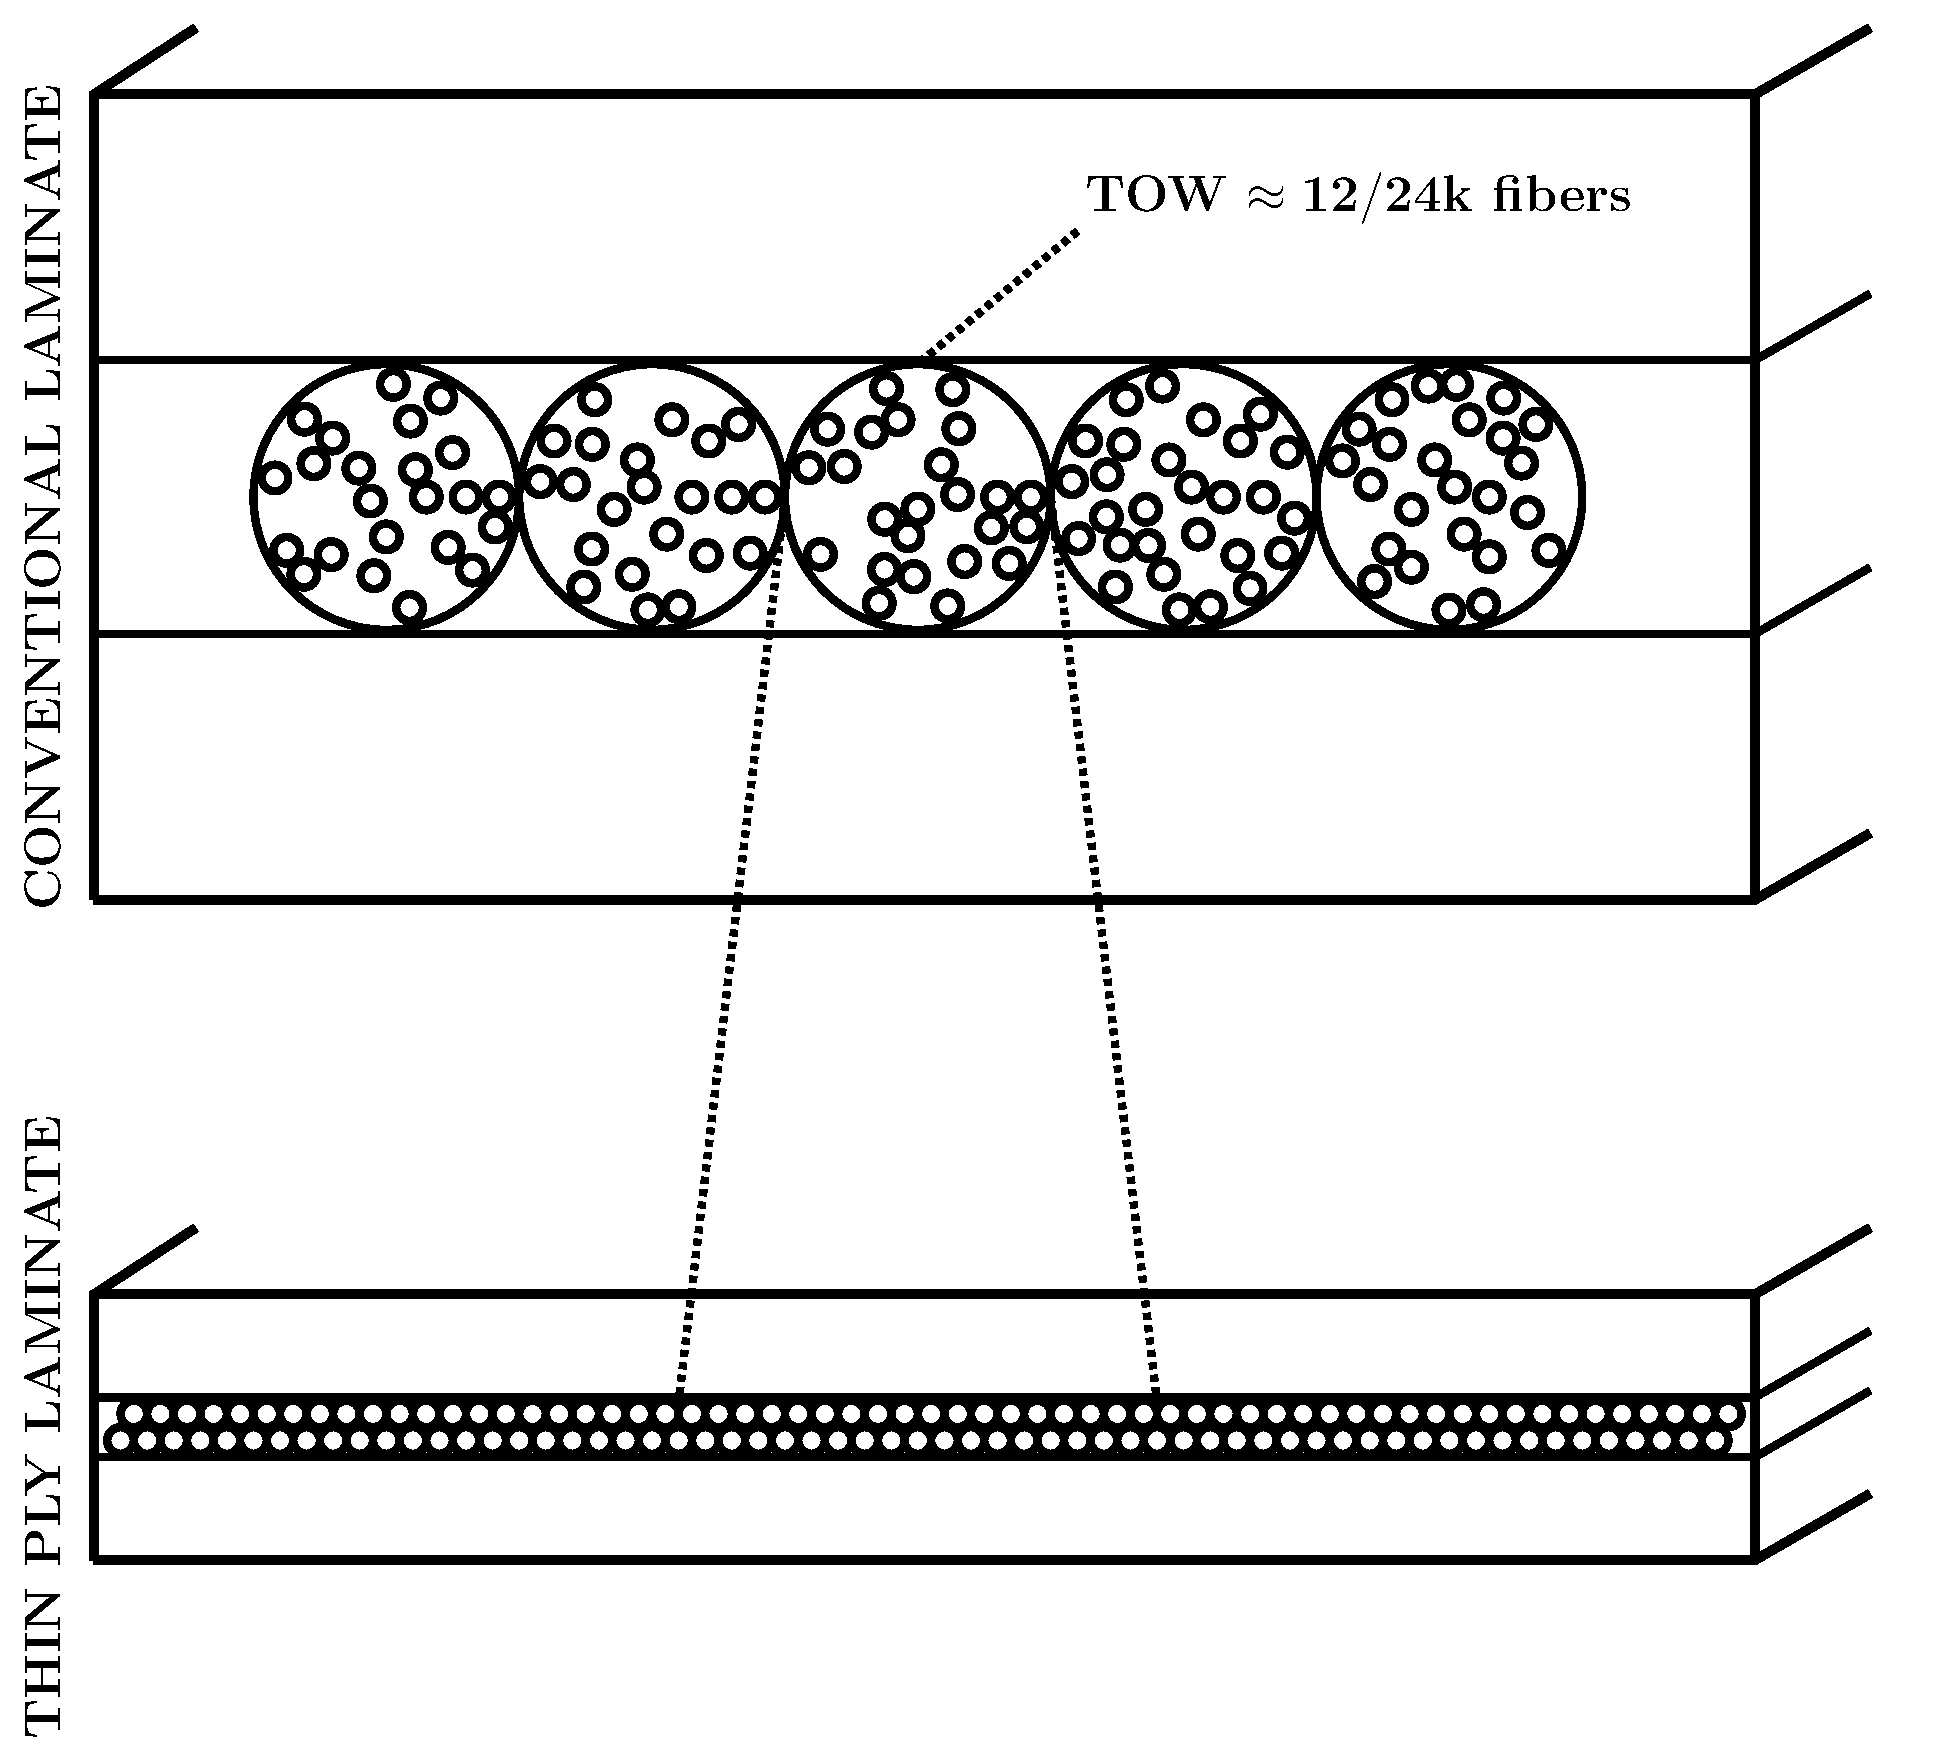
\includegraphics[width=0.72\textwidth]{spread-tow-tech.pdf}
\end{figure}
\end{frame}

\addtocounter{framenumber}{-1}

\begin{frame}
\frametitle{\vspace{0.3cm}\small The Thin-ply ``Advantage'': new material}
\vspace{-0.8cm}
\centering
\begin{columns}[t]
\begin{column}{0.5\textwidth}
\centering
\tiny
\textbf{2018}, $\mathbf{\left[45^{\circ}, 90^{\circ},-45^{\circ},0^{\circ}\right]_{nS}}$
\end{column}
\begin{column}{0.5\textwidth}
\centering

\end{column}
\end{columns}
\vspace{-0.4cm}
\begin{columns}[c]
\begin{column}{0.5\textwidth}
\begin{figure}
\centering
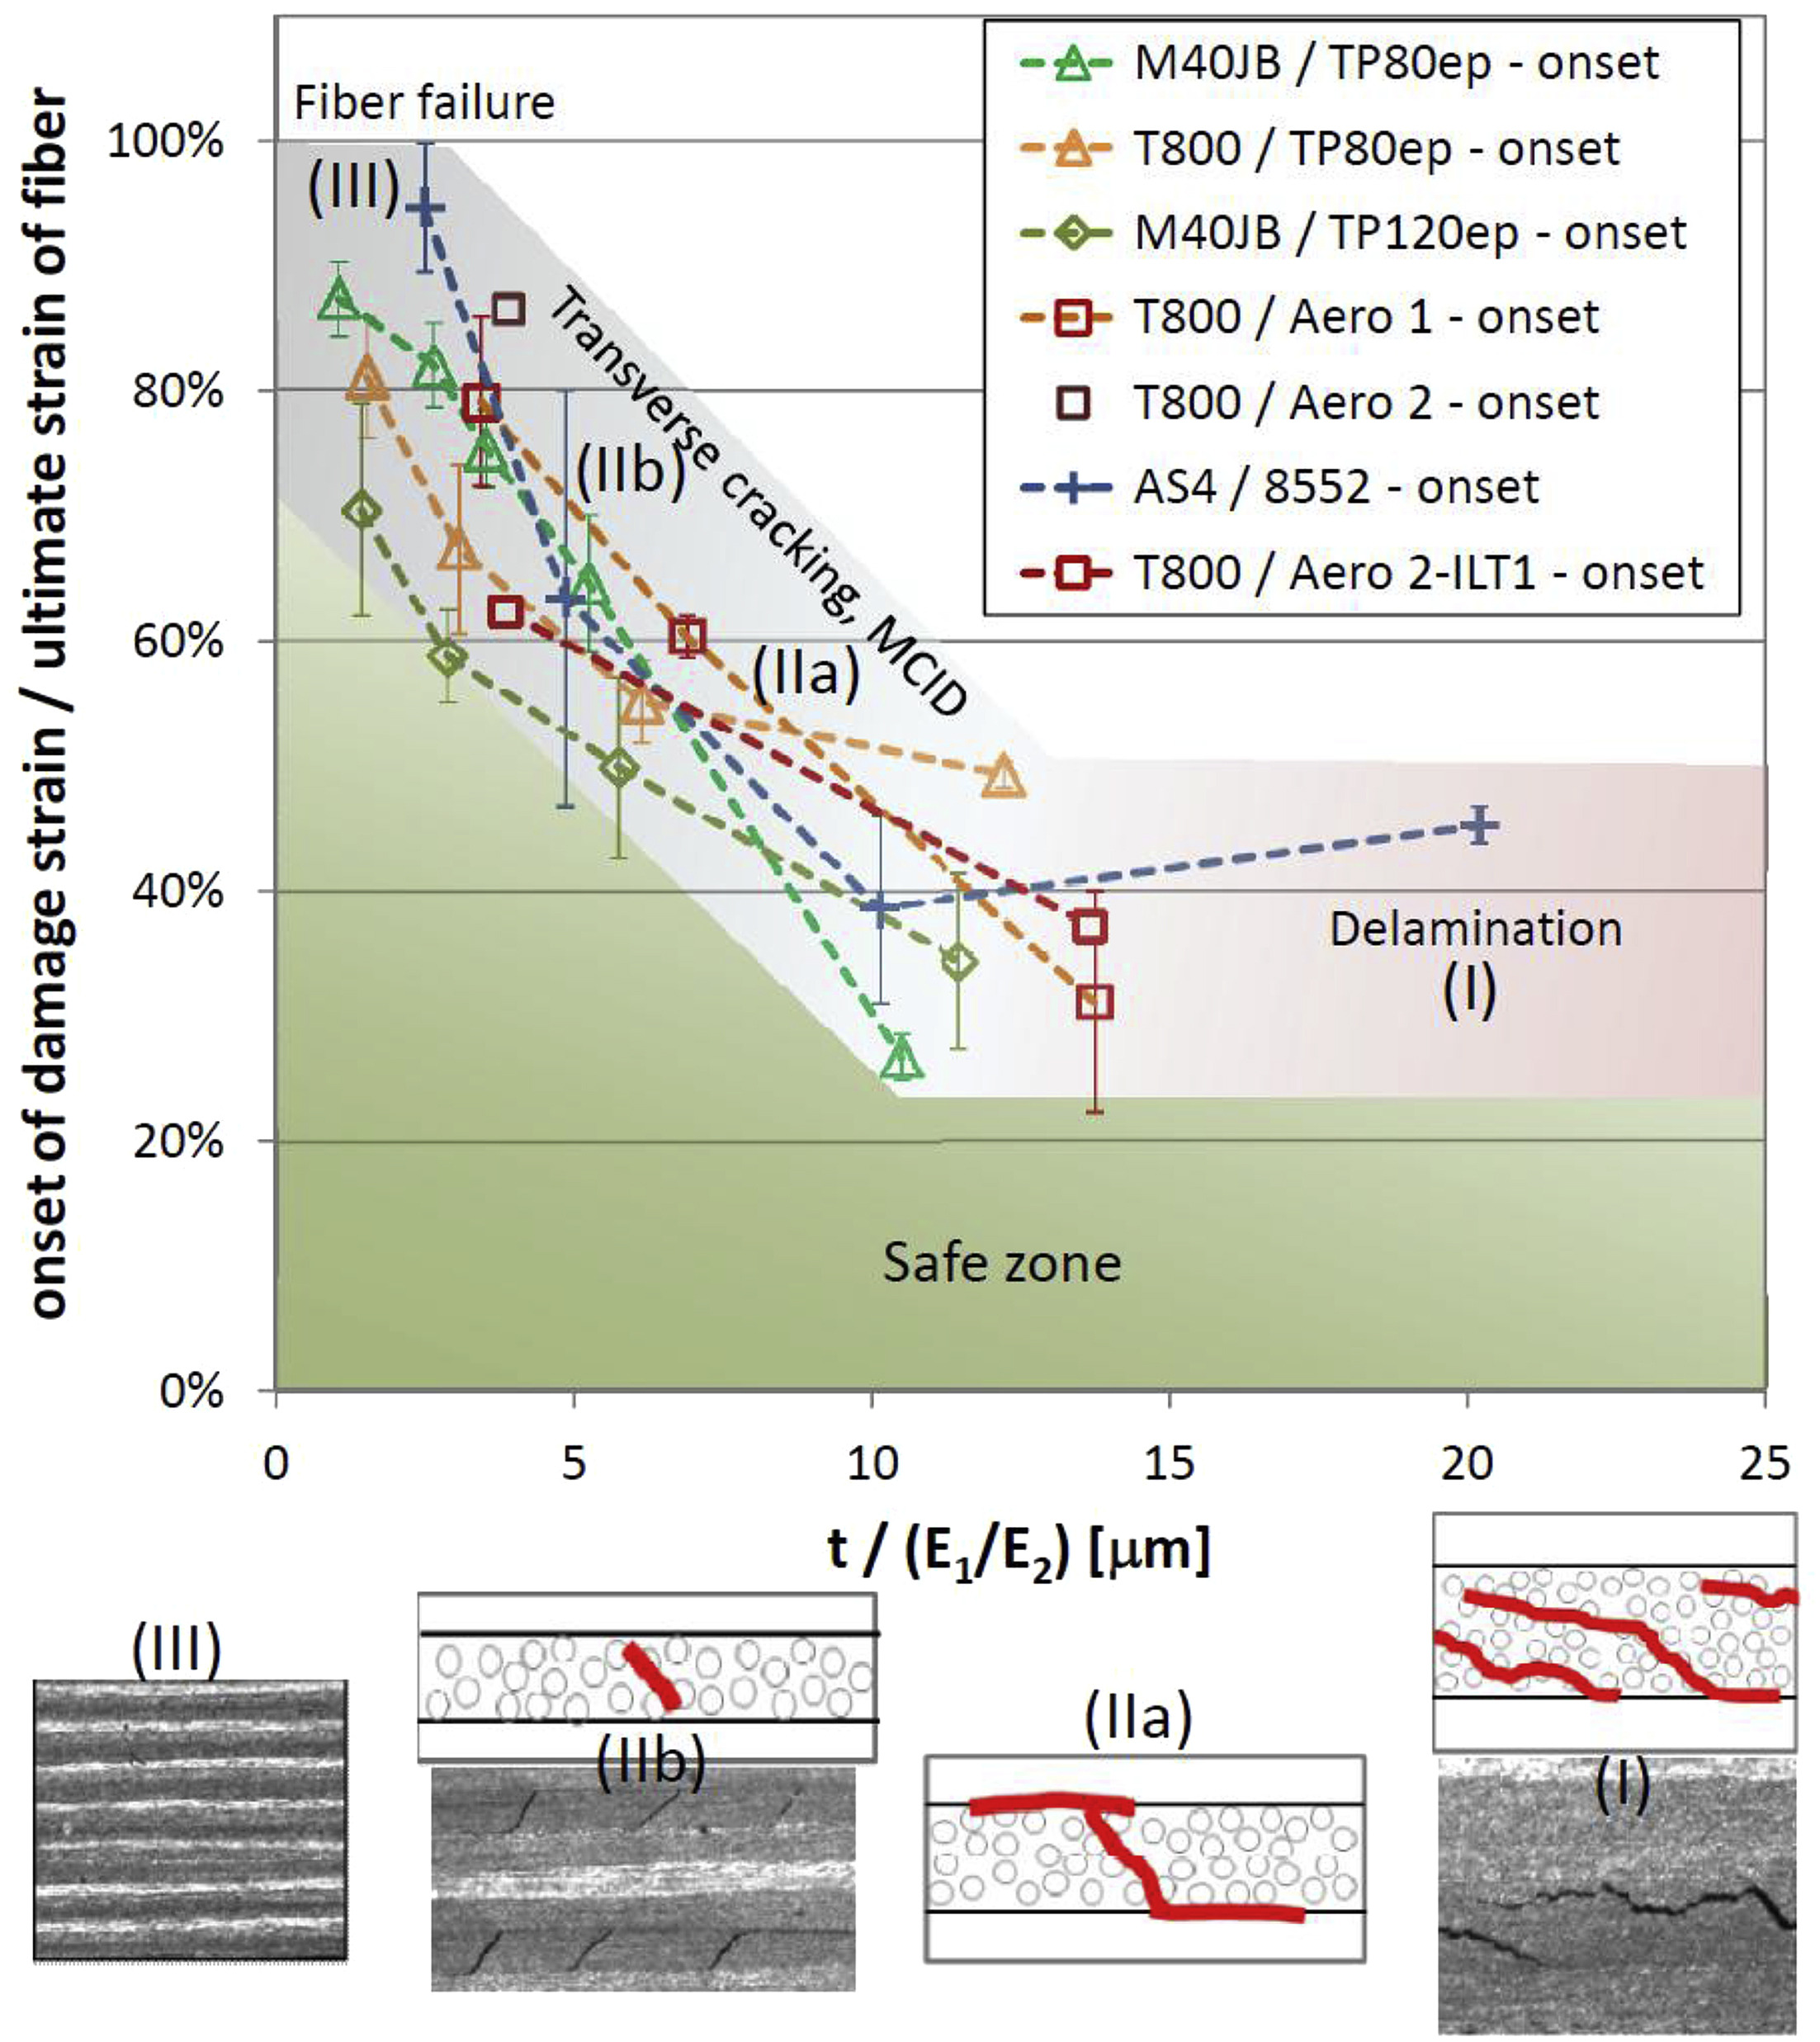
\includegraphics[width=0.9\columnwidth]{thinply-plythicknesseffect.jpg}
\end{figure}
\vspace{-0.6cm}
\centering
\textcolor{white}{\tiny$t_{90^{\circ}}<10\diameter_{fiber}$}
\end{column}
\begin{column}{0.5\textwidth}
\centering
\end{column}
\end{columns}
\vspace{0.15cm}
\begin{columns}[b]
\begin{column}{0.5\textwidth}
\centering
\pgfmathsetmacro\fontsizeref{4.5}
\pgfmathsetmacro\stretchref{1}
{\fontsize{\fontsizeref}{\stretchref} \selectfont \href{https://doi.org/10.1016/j.compscitech.2018.08.037}{Cugnoni et al., Compos. Sci. Technol. \textbf{168}, 2018.}}
\end{column}
\begin{column}{0.5\textwidth}
\centering
\end{column}
\end{columns}
\end{frame}

\addtocounter{framenumber}{-1}

\begin{frame}
\frametitle{\vspace{0.3cm}\small The Thin-ply ``Advantage'': new material, old result}
\vspace{-0.8cm}
\centering
\begin{columns}[t]
\begin{column}{0.5\textwidth}
\centering
\tiny
\textbf{2018}, $\mathbf{\left[45^{\circ}, 90^{\circ},-45^{\circ},0^{\circ}\right]_{nS}}$
\end{column}
\begin{column}{0.5\textwidth}
\centering
\tiny
\textbf{1979}, $\mathbf{\left[0^{\circ}, 90^{\circ}_{n}\right]_{S}}$
\end{column}
\end{columns}
\vspace{-0.4cm}
\begin{columns}[c]
\begin{column}{0.5\textwidth}
\begin{figure}
\centering
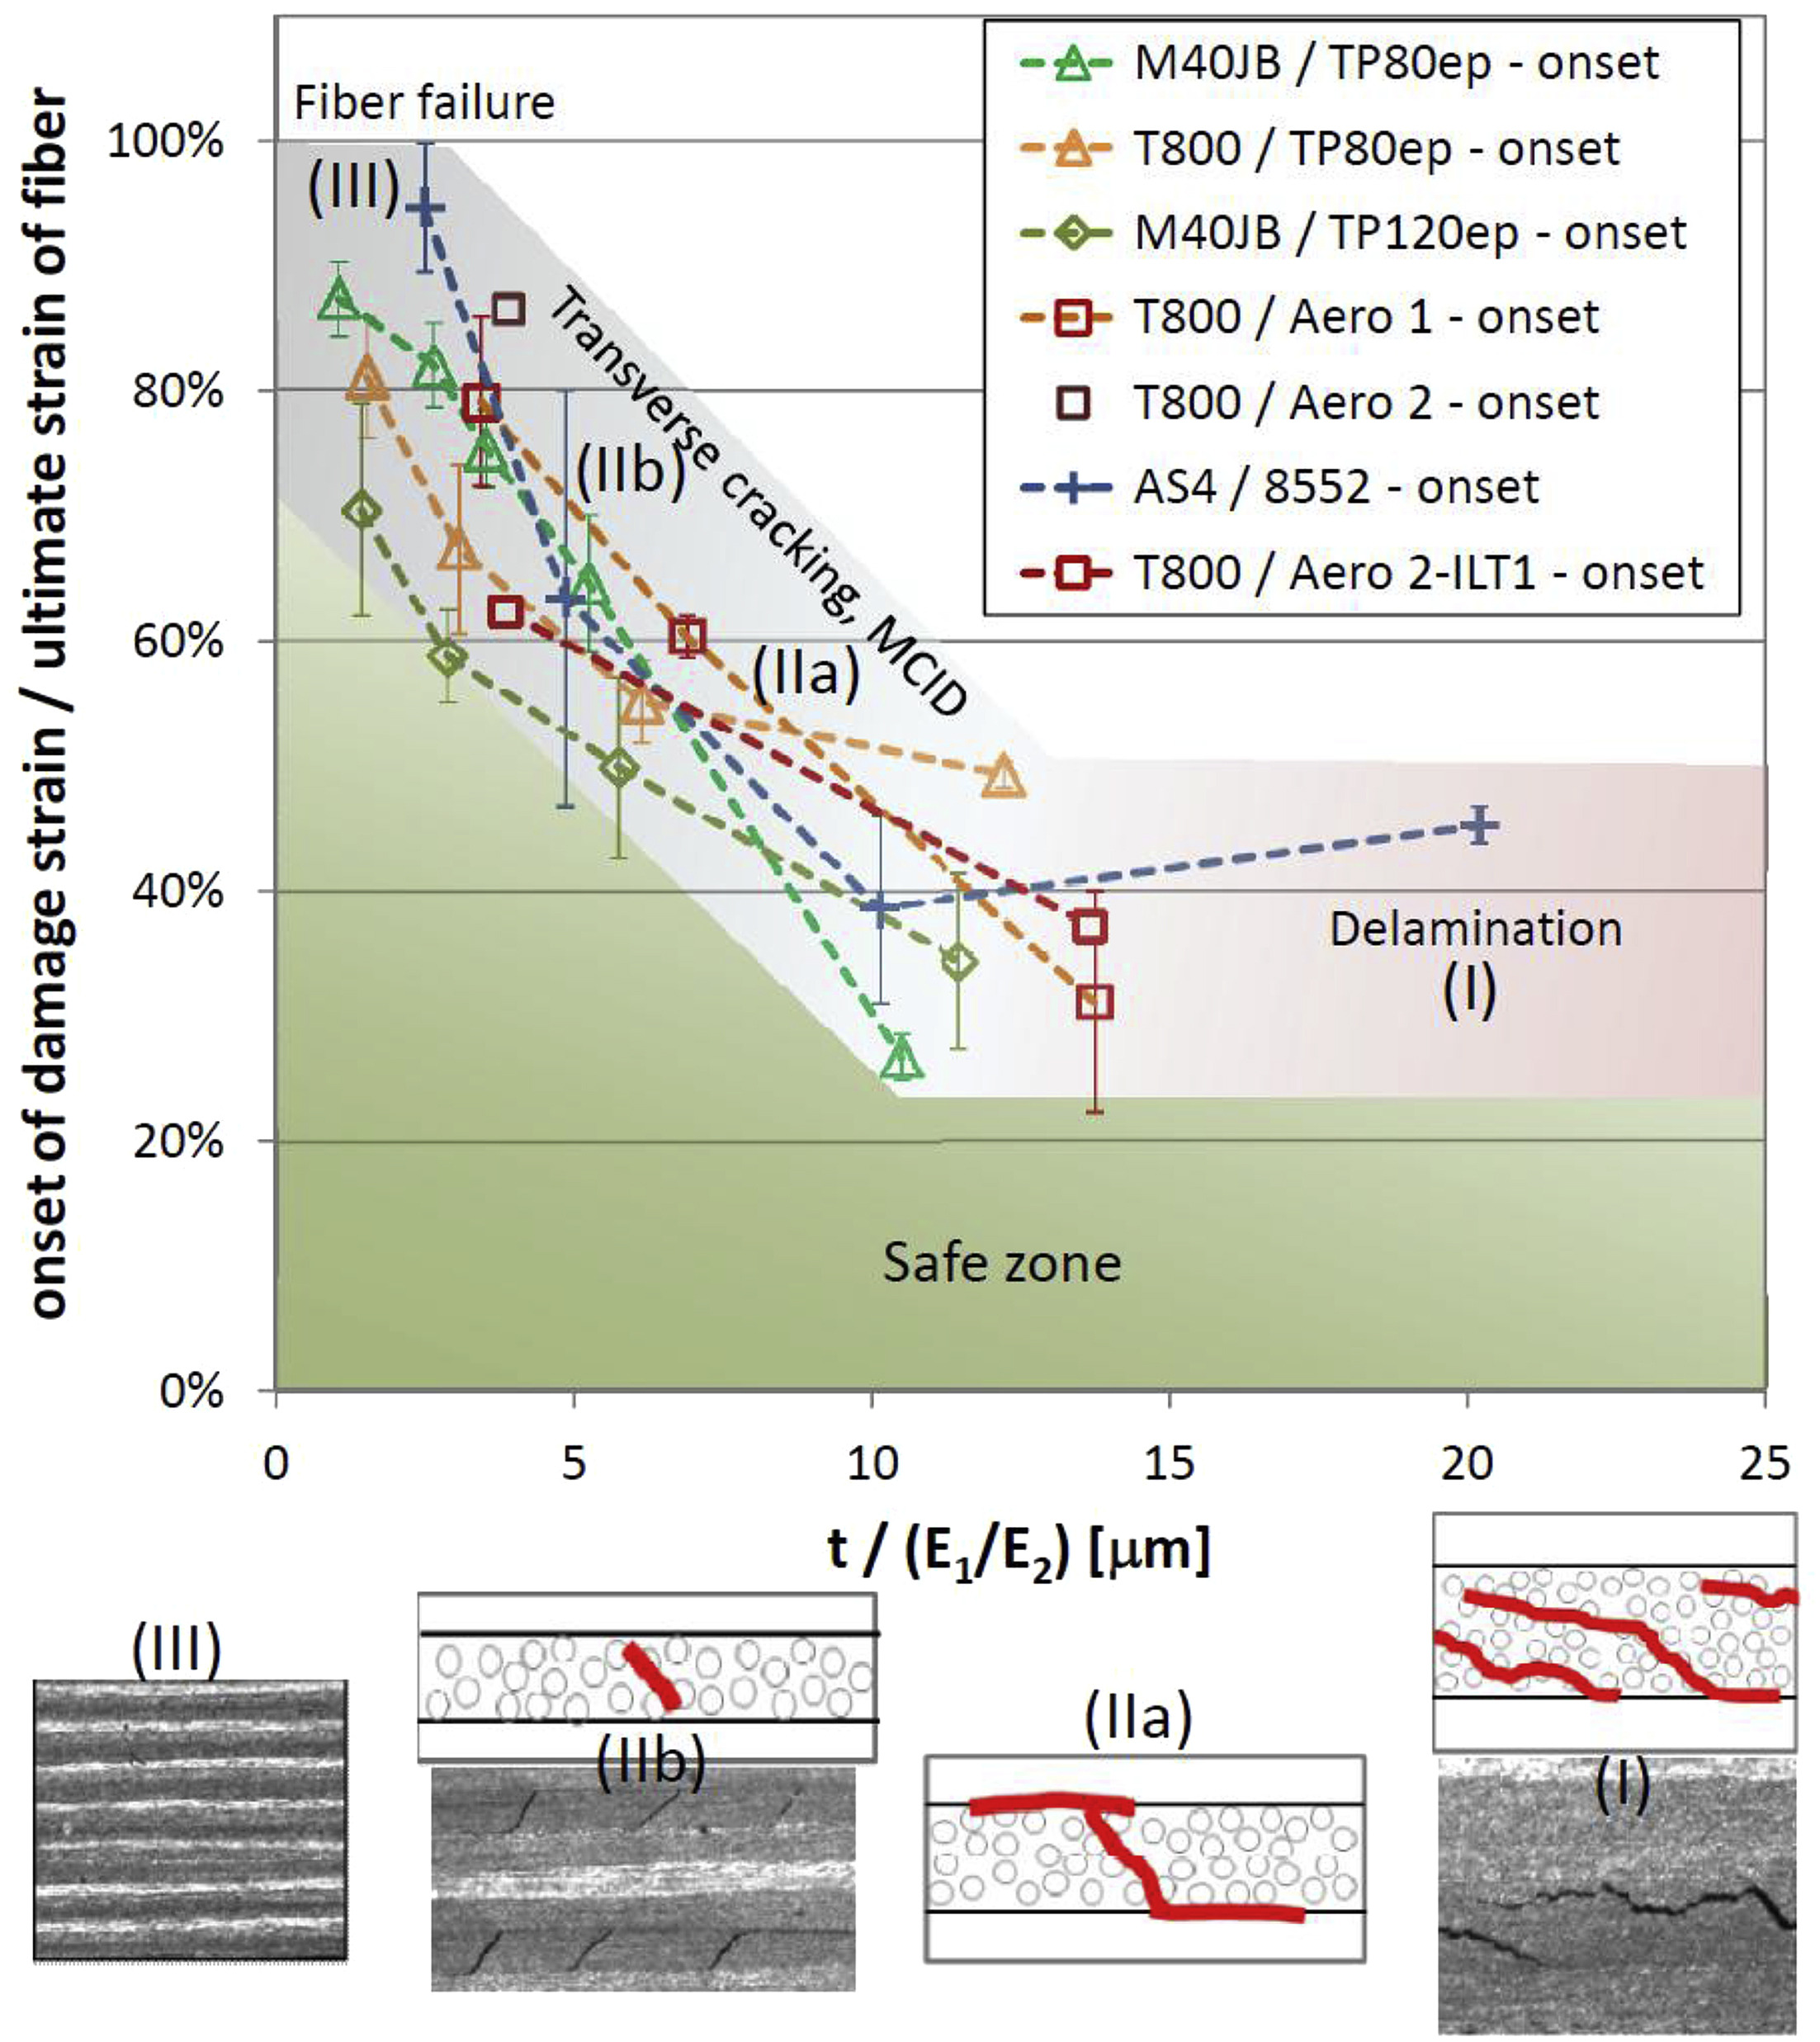
\includegraphics[width=0.9\columnwidth]{thinply-plythicknesseffect.jpg}
\end{figure}
\vspace{-0.6cm}
\centering
\textcolor{white}{\tiny$t_{90^{\circ}}<10\diameter_{fiber}$}
\end{column}
\begin{column}{0.5\textwidth}
\centering
\begin{figure}
\centering
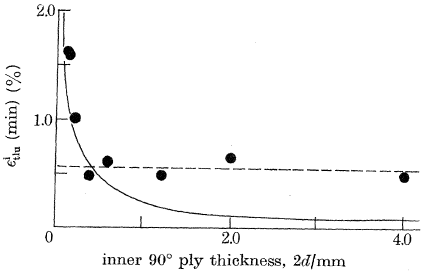
\includegraphics[width=\columnwidth]{bailey.png}
\end{figure}
\textcolor{white}{\tiny$t_{90^{\circ}}>100\diameter_{fiber}$}
\end{column}
\end{columns}
\vspace{0.15cm}
\begin{columns}[b]
\begin{column}{0.5\textwidth}
\centering
\pgfmathsetmacro\fontsizeref{4.5}
\pgfmathsetmacro\stretchref{1}
{\fontsize{\fontsizeref}{\stretchref} \selectfont \href{https://doi.org/10.1016/j.compscitech.2018.08.037}{Cugnoni et al., Compos. Sci. Technol. \textbf{168}, 2018.}}
\end{column}
\begin{column}{0.5\textwidth}
\centering
\pgfmathsetmacro\fontsizeref{4.5}
\pgfmathsetmacro\stretchref{1}
{\fontsize{\fontsizeref}{\stretchref} \selectfont \href{https://doi.org/10.1098/rspa.1979.0071}{Bailey et al., P. Roy. Soc. A-Math. Phy. \textbf{366} (1727), 1979.}}
\end{column}
\end{columns}
\end{frame}

\addtocounter{framenumber}{-1}

\begin{frame}
\frametitle{\vspace{0.3cm}\small The Thin-ply ``Advantage'': new material, old result?}
\vspace{-0.8cm}
\centering
\begin{columns}[t]
\begin{column}{0.5\textwidth}
\centering
\tiny
\textbf{2018}, $\mathbf{\left[45^{\circ}, 90^{\circ},-45^{\circ},0^{\circ}\right]_{nS}}$
\end{column}
\begin{column}{0.5\textwidth}
\centering
\tiny
\textbf{1979}, $\mathbf{\left[0^{\circ}, 90^{\circ}_{n}\right]_{S}}$
\end{column}
\end{columns}
\vspace{-0.4cm}
\begin{columns}[c]
\begin{column}{0.5\textwidth}
\begin{figure}
\centering
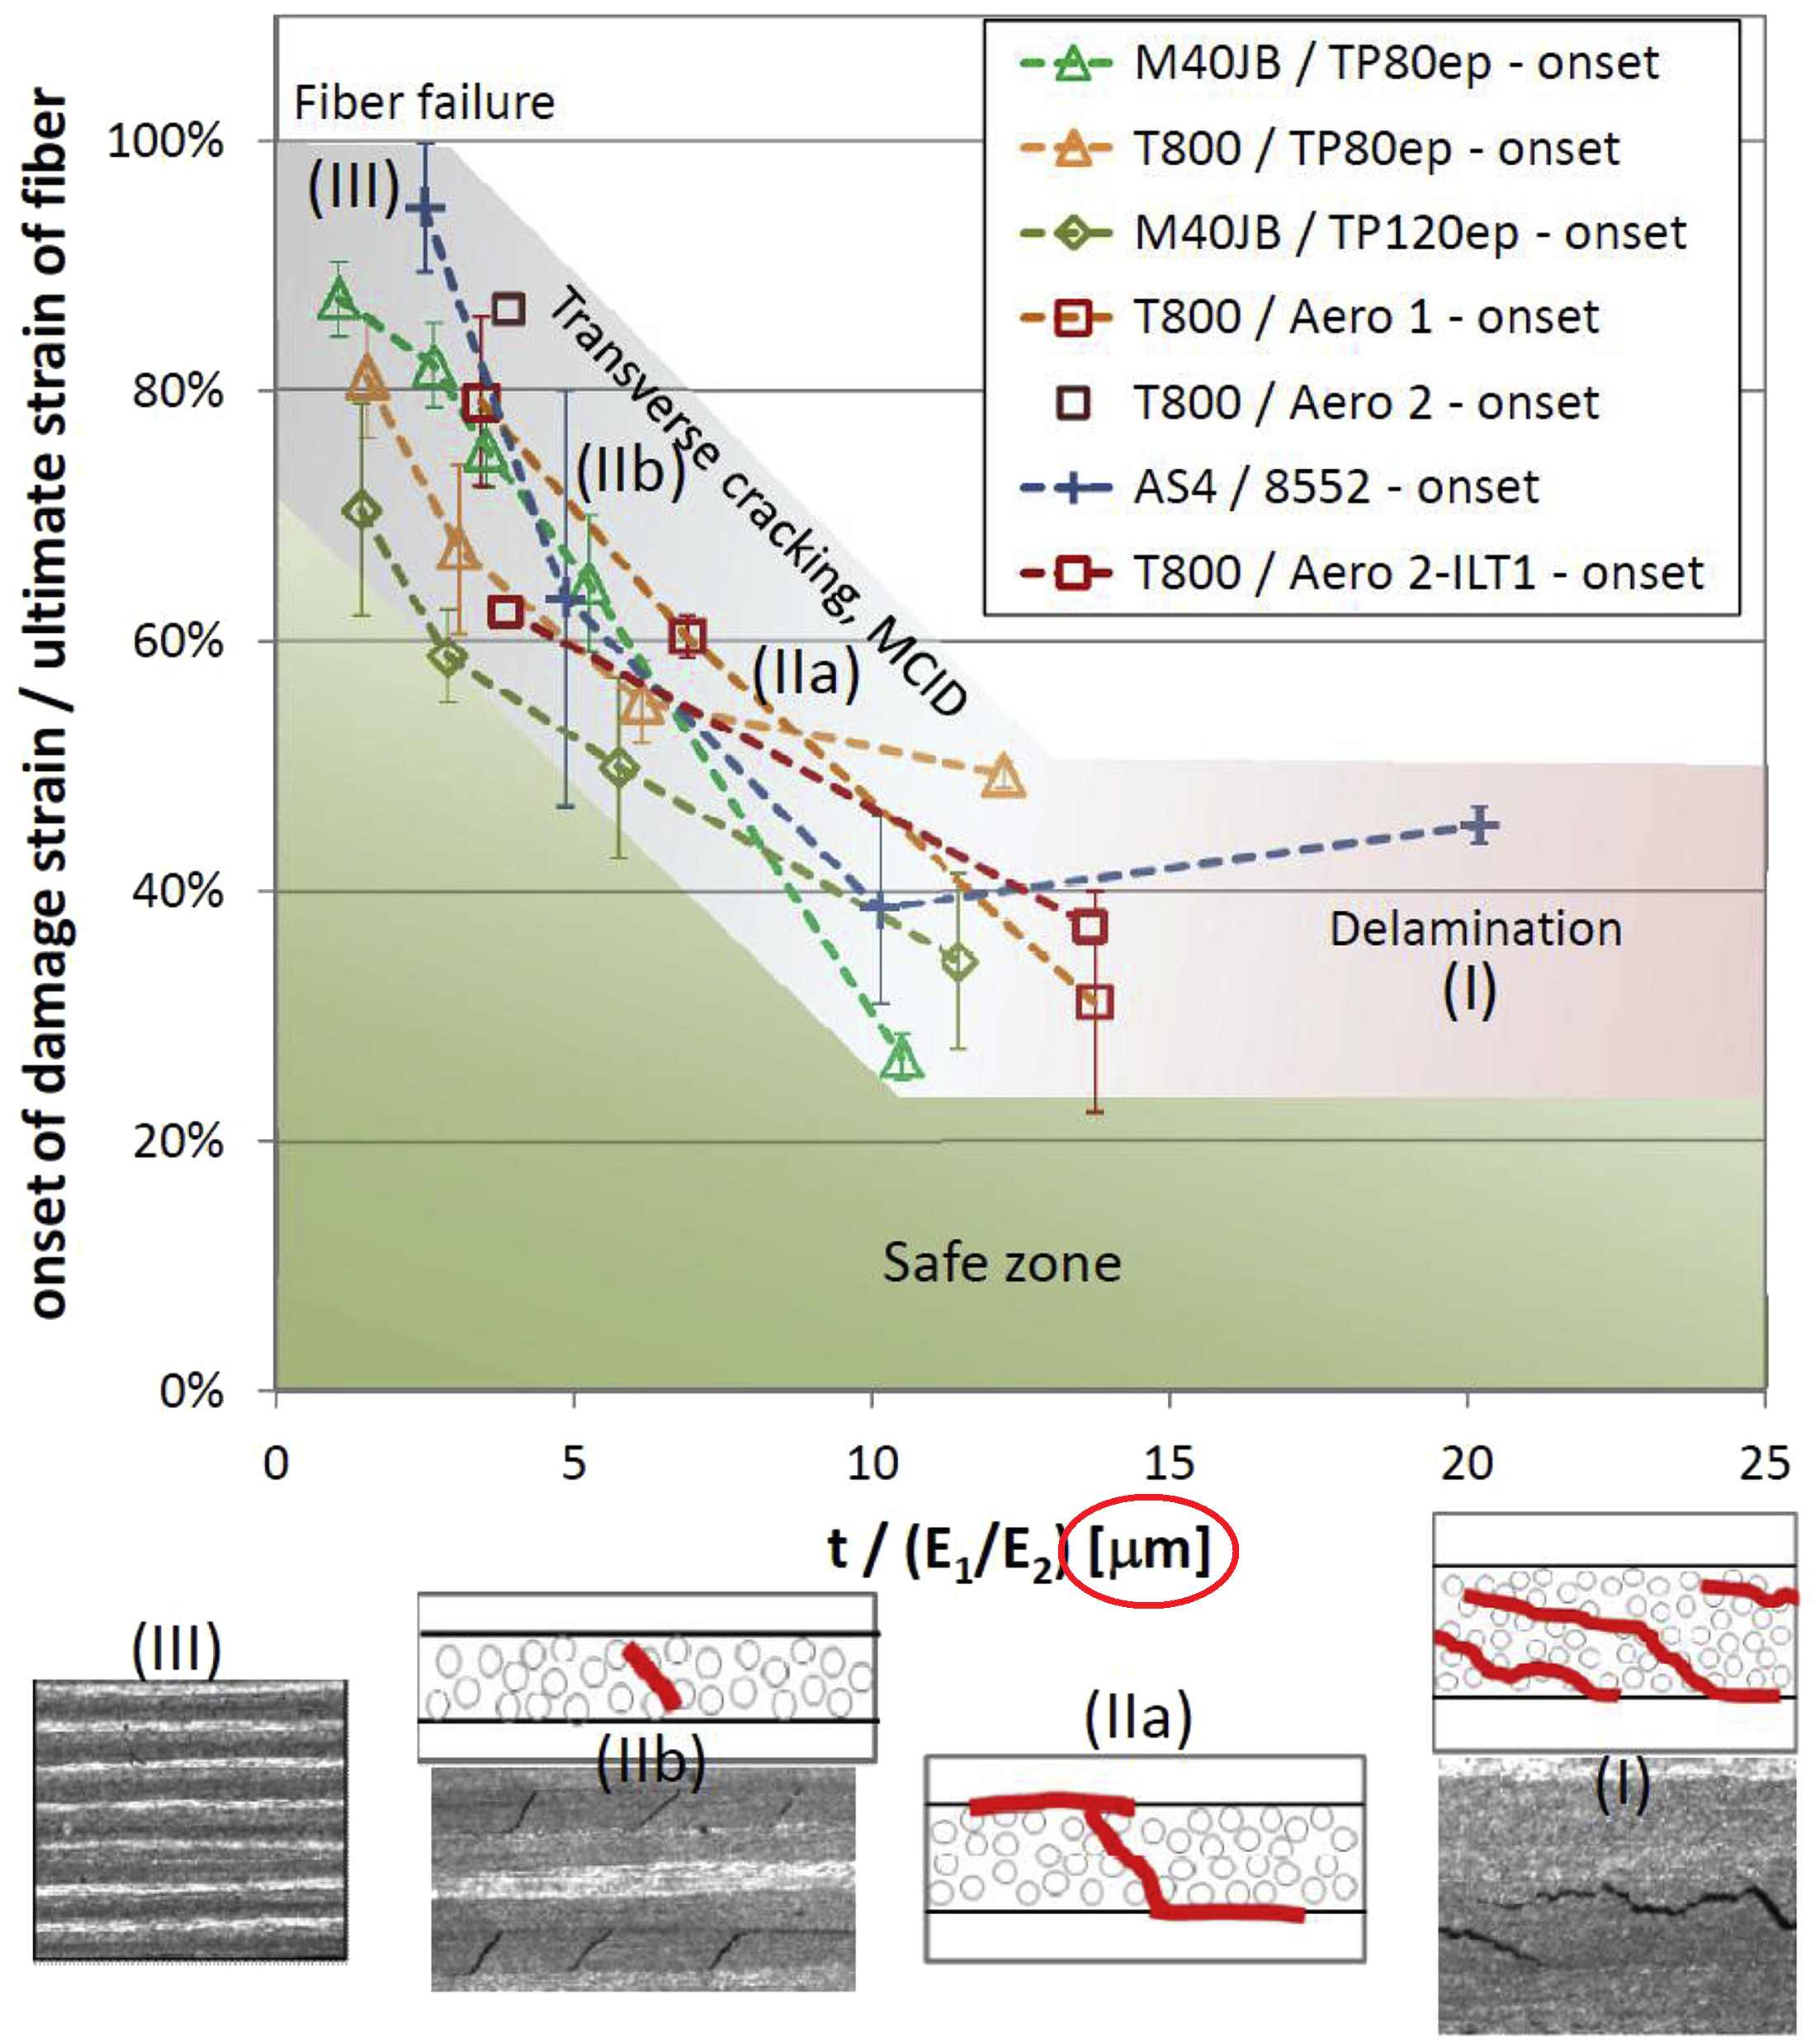
\includegraphics[width=0.9\columnwidth]{thinply-plythicknesseffect-highlighted.png}
\end{figure}
\vspace{-0.6cm}
\centering
\textcolor{red}{\tiny$t_{90^{\circ}}<10\diameter_{fiber}$}
\end{column}
\begin{column}{0.5\textwidth}
\centering
\begin{figure}
\centering
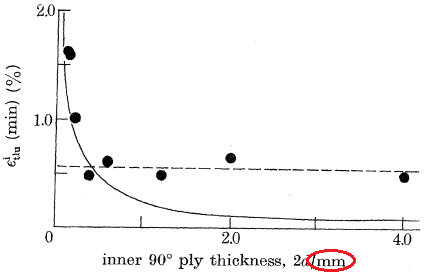
\includegraphics[width=\columnwidth]{bailey-highlighted.png}
\end{figure}
\textcolor{red}{\tiny$t_{90^{\circ}}>100\diameter_{fiber}$}
\end{column}
\end{columns}
\vspace{0.15cm}
\begin{columns}[b]
\begin{column}{0.5\textwidth}
\centering
\pgfmathsetmacro\fontsizeref{4.5}
\pgfmathsetmacro\stretchref{1}
{\fontsize{\fontsizeref}{\stretchref} \selectfont \href{https://doi.org/10.1016/j.compscitech.2018.08.037}{Cugnoni et al., Compos. Sci. Technol. \textbf{168}, 2018.}}
\end{column}
\begin{column}{0.5\textwidth}
\centering
\pgfmathsetmacro\fontsizeref{4.5}
\pgfmathsetmacro\stretchref{1}
{\fontsize{\fontsizeref}{\stretchref} \selectfont \href{https://doi.org/10.1098/rspa.1979.0071}{Bailey et al., P. Roy. Soc. A-Math. Phy. \textbf{366} (1727), 1979.}}
\end{column}
\end{columns}
\end{frame}

\subsection{Micromechanics of Initiation}

\begin{frame}
\frametitle{\vspace{0.3cm}\small Micromechanics of Initiation}
\vspace{-0.5cm}
\centering
\captionsetup[subfigure]{labelfont=footnotesize}
\begin{tikzpicture}

%Tikz axis starts%

\draw[->,black, line width = 5pt] (-4,0) -- (-4,3);
\draw[->,black, line width = 5pt] (-4,0) -- (-4,-3);
\node  at (-4,0) {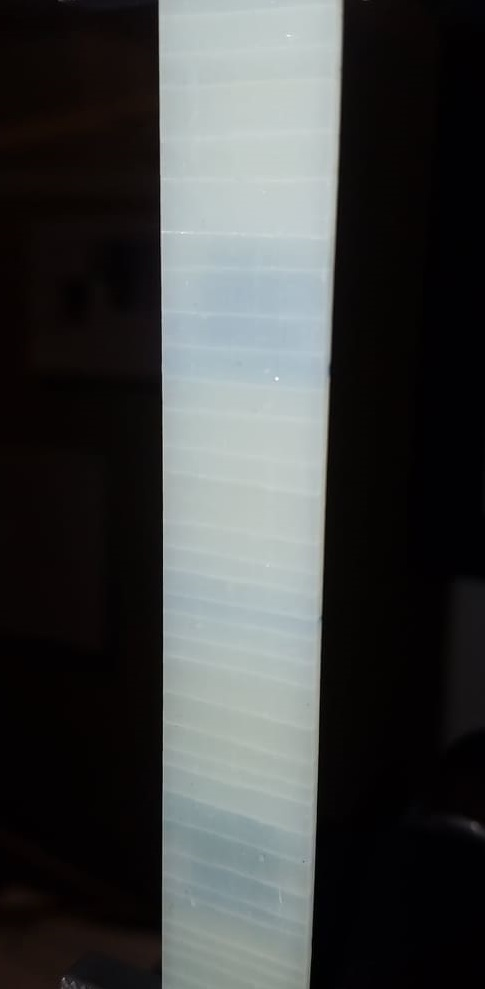
\includegraphics[height=0.6\textheight]{0-90_2_symm}};
\draw[<->,red, line width = 1.25pt] (-4.35,-0.5) -- (-3.65,-0.625);
\node[red, below]  at (-4,-0.65) {\tiny$\mathbf{\sim 15\ mm}$};
\node[above, right]  at (-3.8,3) {\Huge$\mathbf{\varepsilon}$};
\node[below, left]  at (-4.2,-3) {\Huge$\mathbf{\varepsilon}$};

\draw[->,black, line width = 5pt] (-2,0) -- (-2,3);
\draw[->,black, line width = 5pt] (-2,0) -- (-2,-3);
\node  at (-2,0) {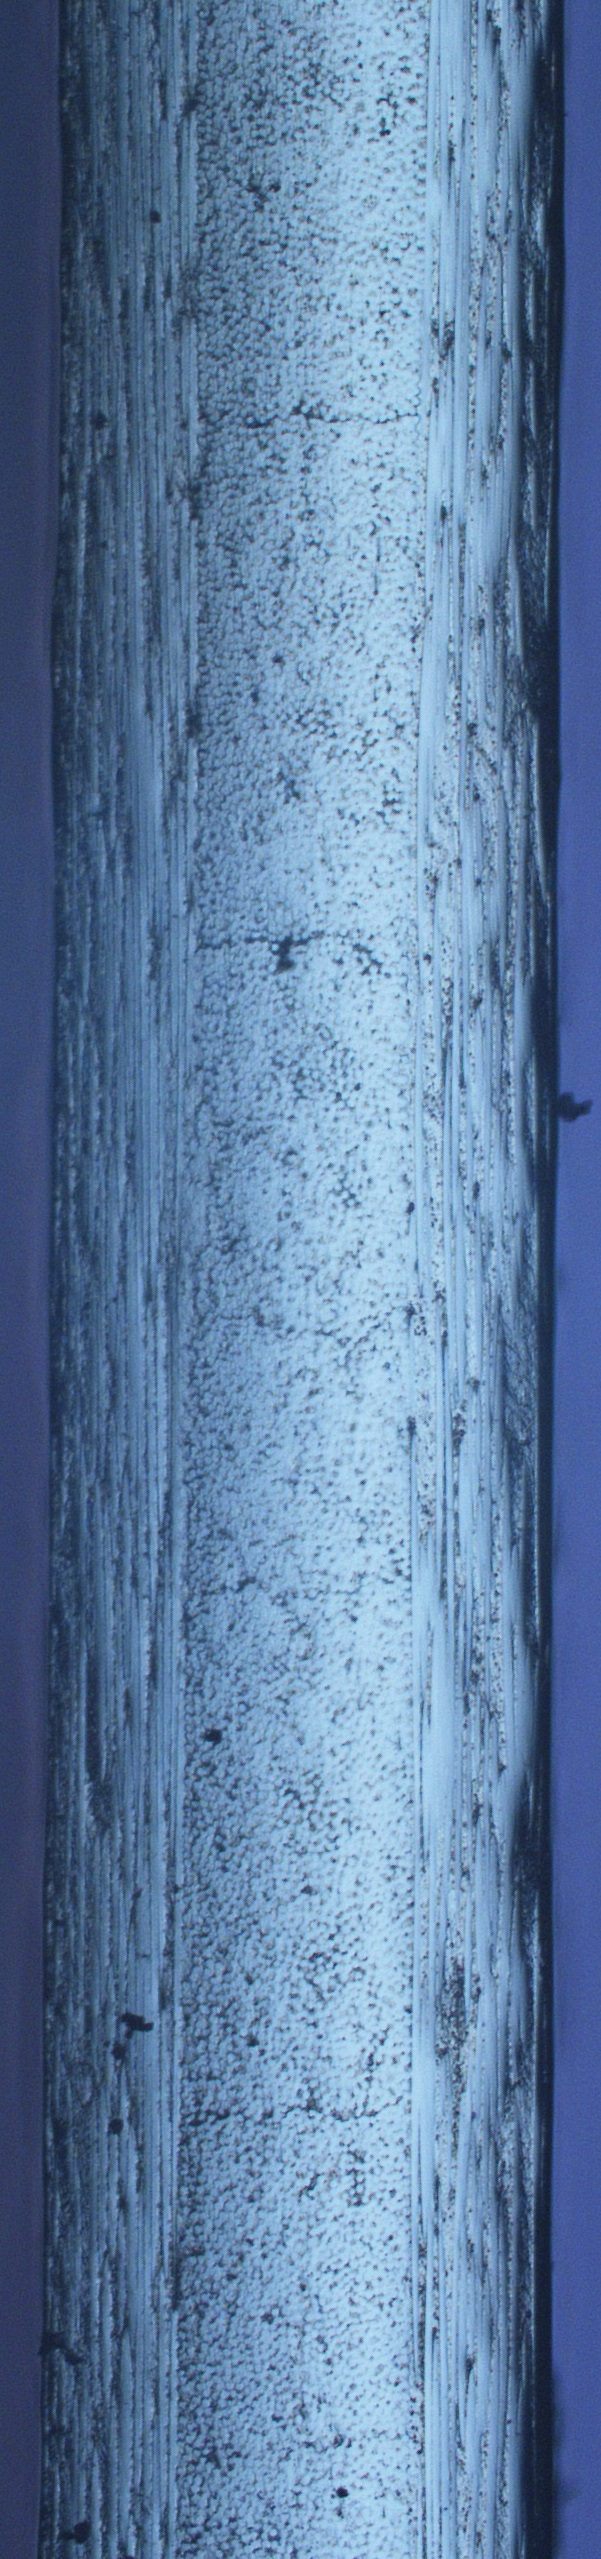
\includegraphics[height=0.6\textheight]{0-90_symm_edge}};
\draw[<->,red, line width = 1.25pt] (-2.46,-0.6) -- (-1.55,-0.6);
\node[red, below]  at (-2,-0.6) {\tiny$\mathbf{\sim 2\ mm}$};
\node[above, right]  at (-1.8,3) {\Huge$\mathbf{\varepsilon}$};
\node[below, left]  at (-2.2,-3) {\Huge$\mathbf{\varepsilon}$};

\draw[->,black, line width = 5pt] (1,0) -- (1,3);
\draw[->,black, line width = 5pt] (1,0) -- (1,-3);
\node  at (1,0) {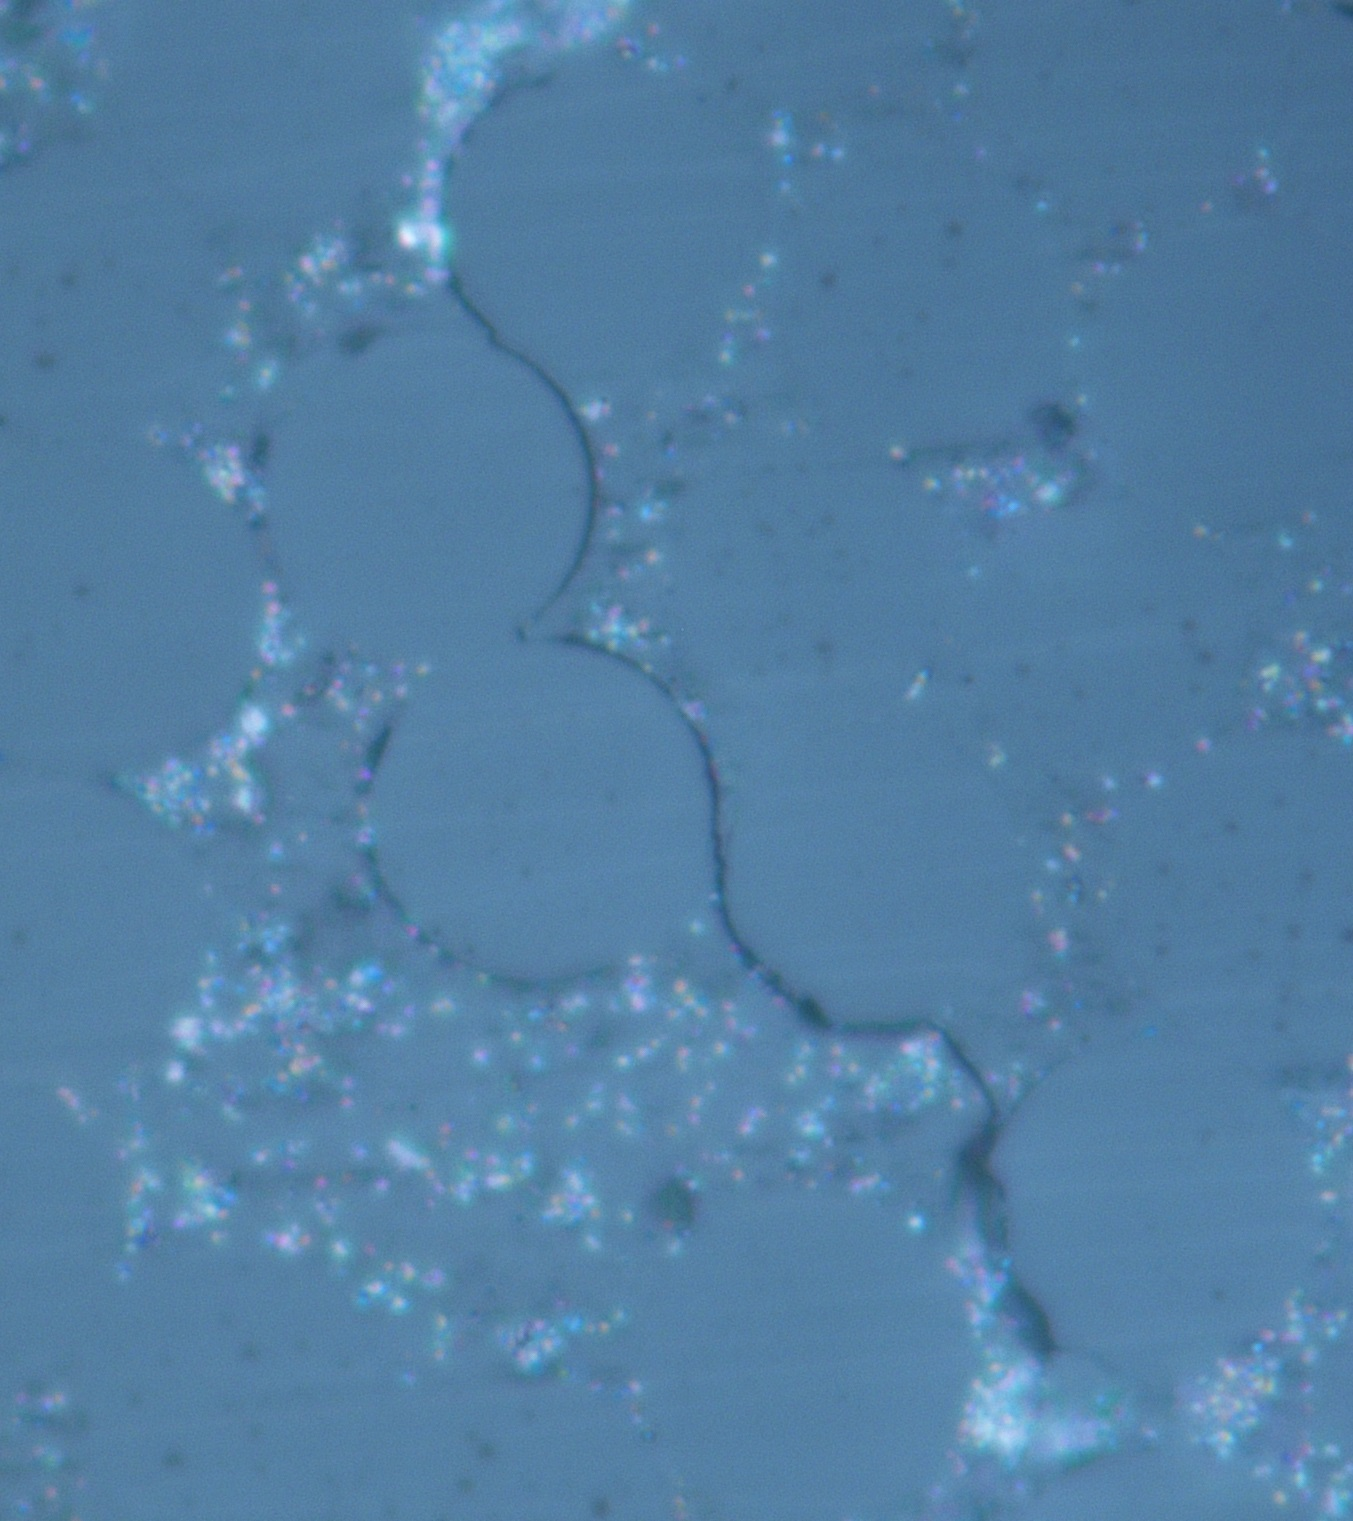
\includegraphics[height=0.6\textheight,width=0.6\textheight,angle=90]{0-90_symm_debondetail}};
\draw[<->,red, line width = 1.25pt] (0.65,-0.45) -- (1.675,-0.45);
\node[red, below]  at (1.05,-0.475) {\tiny$\mathbf{\sim 8\ \mu m}$};
\node[above, right]  at (1.2,3) {\Huge$\mathbf{\varepsilon}$};
\node[below, left]  at (0.8,-3) {\Huge$\mathbf{\varepsilon}$};

\node[anchor=south west]  at (3.25,1.55) {\scriptsize\textbf{Left:}};
\node[anchor=west]  at (3.25,1.5) {\scriptsize front view of $\left[0,90_{2}\right]_{S}$,};
\node[anchor=north west]  at (3.25,1.5) {\scriptsize visual inspection.};

\node[anchor=south west]  at (3.25,0.05) {\scriptsize\textbf{Center:}};
\node[anchor=west]  at (3.25,0) {\scriptsize  edge view of $\left[0,90\right]_{S}$,};
\node[anchor=north west]  at (3.25,0) {\scriptsize optical microscope.};

\node[anchor=south west]  at (3.25,-1.45) {\scriptsize\textbf{Right:}};
\node[anchor=west]  at (3.25,-1.5) {\scriptsize edge view of $\left[0,90\right]_{S}$,};
\node[anchor=north west]  at (3.25,-1.5) {\scriptsize optical microscope.};

%Tikz axis ends%

\end{tikzpicture}
\end{frame}

\begin{frame}
\frametitle{\vspace{0.2cm}\small Micromechanics of Initiation}
\vspace{-0.5cm}
\centering
\begin{alertblock}{\centering\scriptsize\bf Stage 1: isolated debonds}
\vspace{-0.25cm}
\begin{figure}
\centering
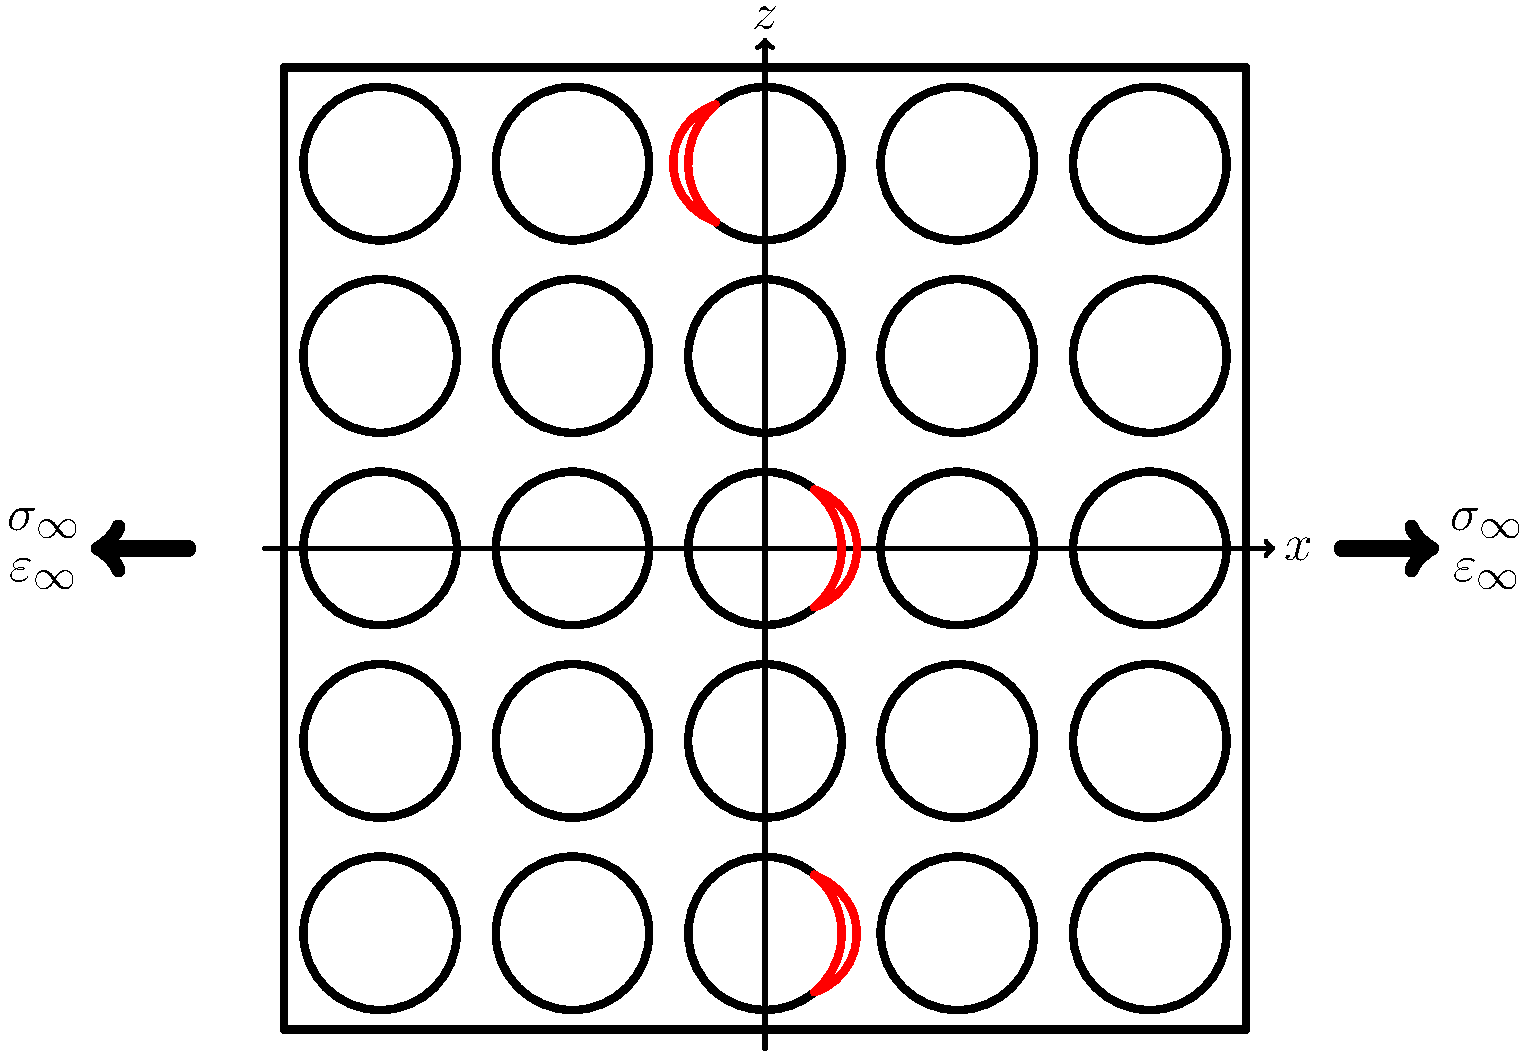
\includegraphics[width=0.6\textwidth]{stage1-isolateddebonds.pdf}
\end{figure}
\end{alertblock}
\vspace{-0.5cm}
\centering
\pgfmathsetmacro\fontsizeref{4.5}
\pgfmathsetmacro\stretchref{1}
{\centering\fontsize{\fontsizeref}{\stretchref} \selectfont \href{https://doi.org/10.1098/rspa.1979.0071}{Bailey et al., P. Roy. Soc. A-Math. Phy. \textbf{366} (1727), 1979.}}\\\vspace{-5pt}
{\centering\fontsize{\fontsizeref}{\stretchref} \selectfont \href{https://doi.org/10.1007/BF00552203}{Bailey et al., J. Mater. Sci. \textbf{16} (3), 1981.}}\\\vspace{-5pt}
{\centering\fontsize{\fontsizeref}{\stretchref} \selectfont \href{https://doi.org/10.1016/S1359-835X(96)00123-6}{Zhang et al., Compos. Part A-Appl. S. \textbf{28} (4), 1997.}}
\end{frame}

\addtocounter{framenumber}{-1}

\begin{frame}
\frametitle{\vspace{0.2cm}\small Micromechanics of Initiation}
\vspace{-0.5cm}
\centering
\begin{alertblock}{\centering\scriptsize\bf Stage 2: consecutive debonds}
\vspace{-0.25cm}
\begin{figure}
\centering
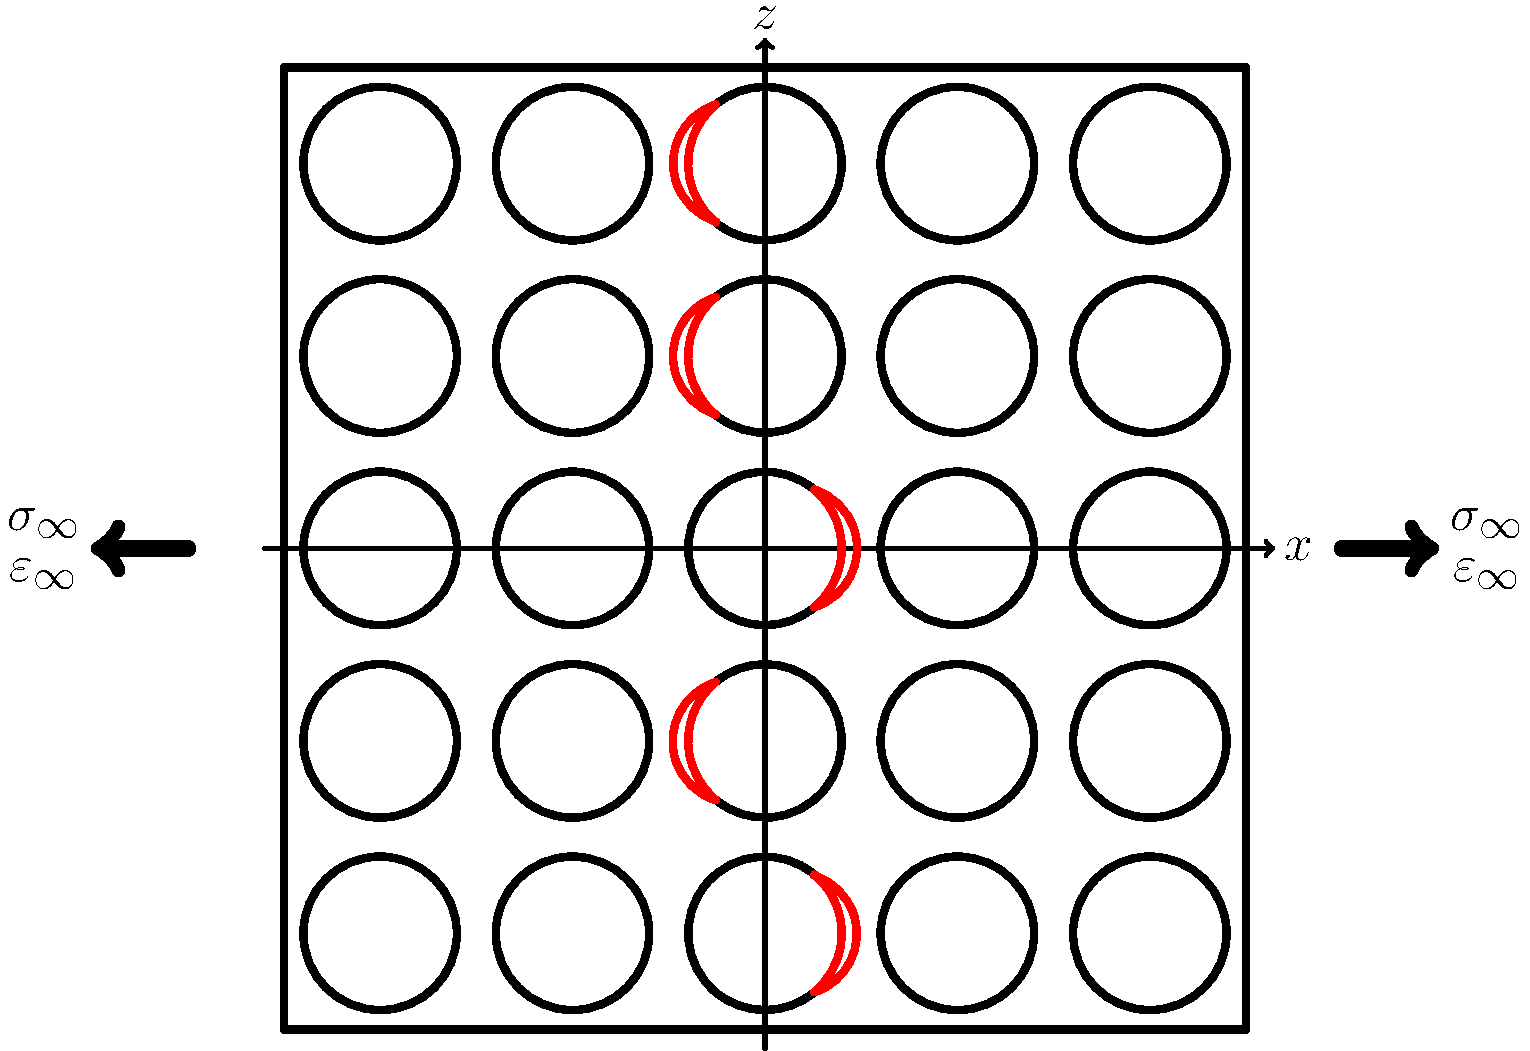
\includegraphics[width=0.6\textwidth]{stage2-critdebonds.pdf}
\end{figure}
\end{alertblock}
\vspace{-0.5cm}
\pgfmathsetmacro\fontsizeref{4.5}
\pgfmathsetmacro\stretchref{1}
{\fontsize{\fontsizeref}{\stretchref} \selectfont \href{https://doi.org/10.1098/rspa.1979.0071}{Bailey et al., P. Roy. Soc. A-Math. Phy. \textbf{366} (1727), 1979.}}\\\vspace{-5pt}
{\fontsize{\fontsizeref}{\stretchref} \selectfont \href{https://doi.org/10.1007/BF00552203}{Bailey et al., J. Mater. Sci. \textbf{16} (3), 1981.}}\\\vspace{-5pt}
{\fontsize{\fontsizeref}{\stretchref} \selectfont \href{https://doi.org/10.1016/S1359-835X(96)00123-6}{Zhang et al., Compos. Part A-Appl. S. \textbf{28} (4), 1997.}}
\end{frame}

\addtocounter{framenumber}{-1}

\begin{frame}
\frametitle{\vspace{0.2cm}\small Micromechanics of Initiation}
\vspace{-0.5cm}
\centering
\begin{alertblock}{\centering\scriptsize\bf Stage 3: kinking}
\vspace{-0.25cm}
\begin{figure}
\centering
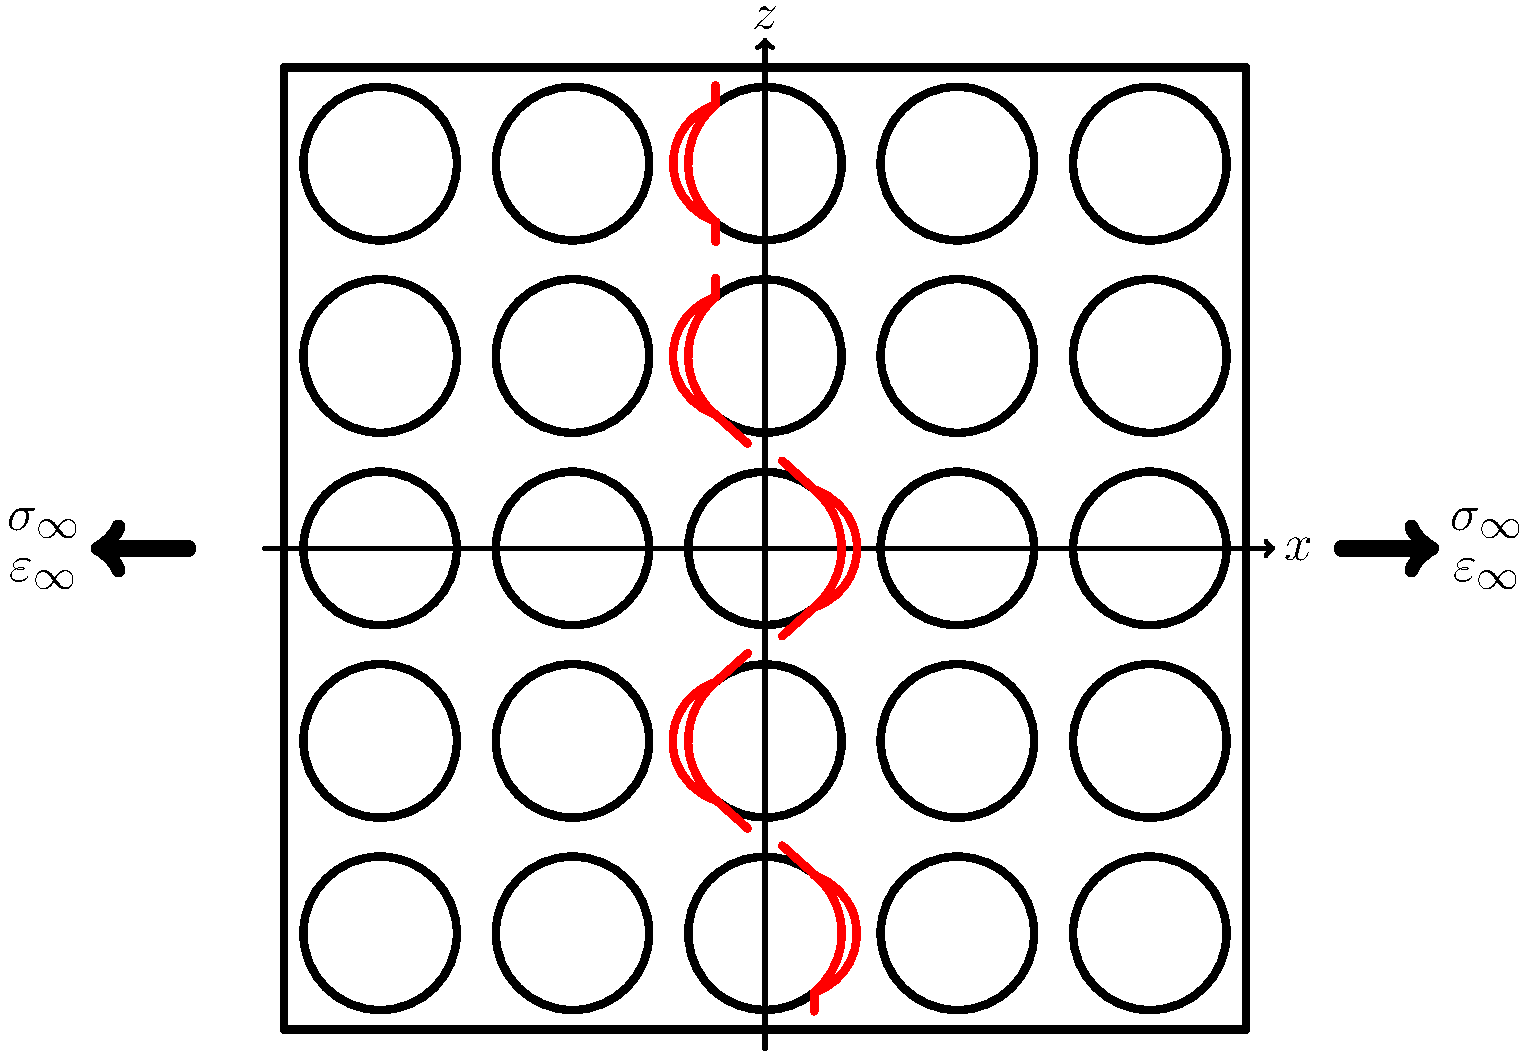
\includegraphics[width=0.6\textwidth]{stage3-kinking.pdf}
\end{figure}
\end{alertblock}
\vspace{-0.5cm}
\pgfmathsetmacro\fontsizeref{4.5}
\pgfmathsetmacro\stretchref{1}
{\fontsize{\fontsizeref}{\stretchref} \selectfont \href{https://doi.org/10.1098/rspa.1979.0071}{Bailey et al., P. Roy. Soc. A-Math. Phy. \textbf{366} (1727), 1979.}}\\\vspace{-5pt}
{\fontsize{\fontsizeref}{\stretchref} \selectfont \href{https://doi.org/10.1007/BF00552203}{Bailey et al., J. Mater. Sci. \textbf{16} (3), 1981.}}\\\vspace{-5pt}
{\fontsize{\fontsizeref}{\stretchref} \selectfont \href{https://doi.org/10.1016/S1359-835X(96)00123-6}{Zhang et al., Compos. Part A-Appl. S. \textbf{28} (4), 1997.}}
\end{frame}

\addtocounter{framenumber}{-1}

\begin{frame}
\frametitle{\vspace{0.2cm}\small Micromechanics of Initiation}
\vspace{-0.5cm}
\centering
\begin{alertblock}{\centering\scriptsize\bf Stage 4: coalescence}
\vspace{-0.25cm}
\begin{figure}
\centering
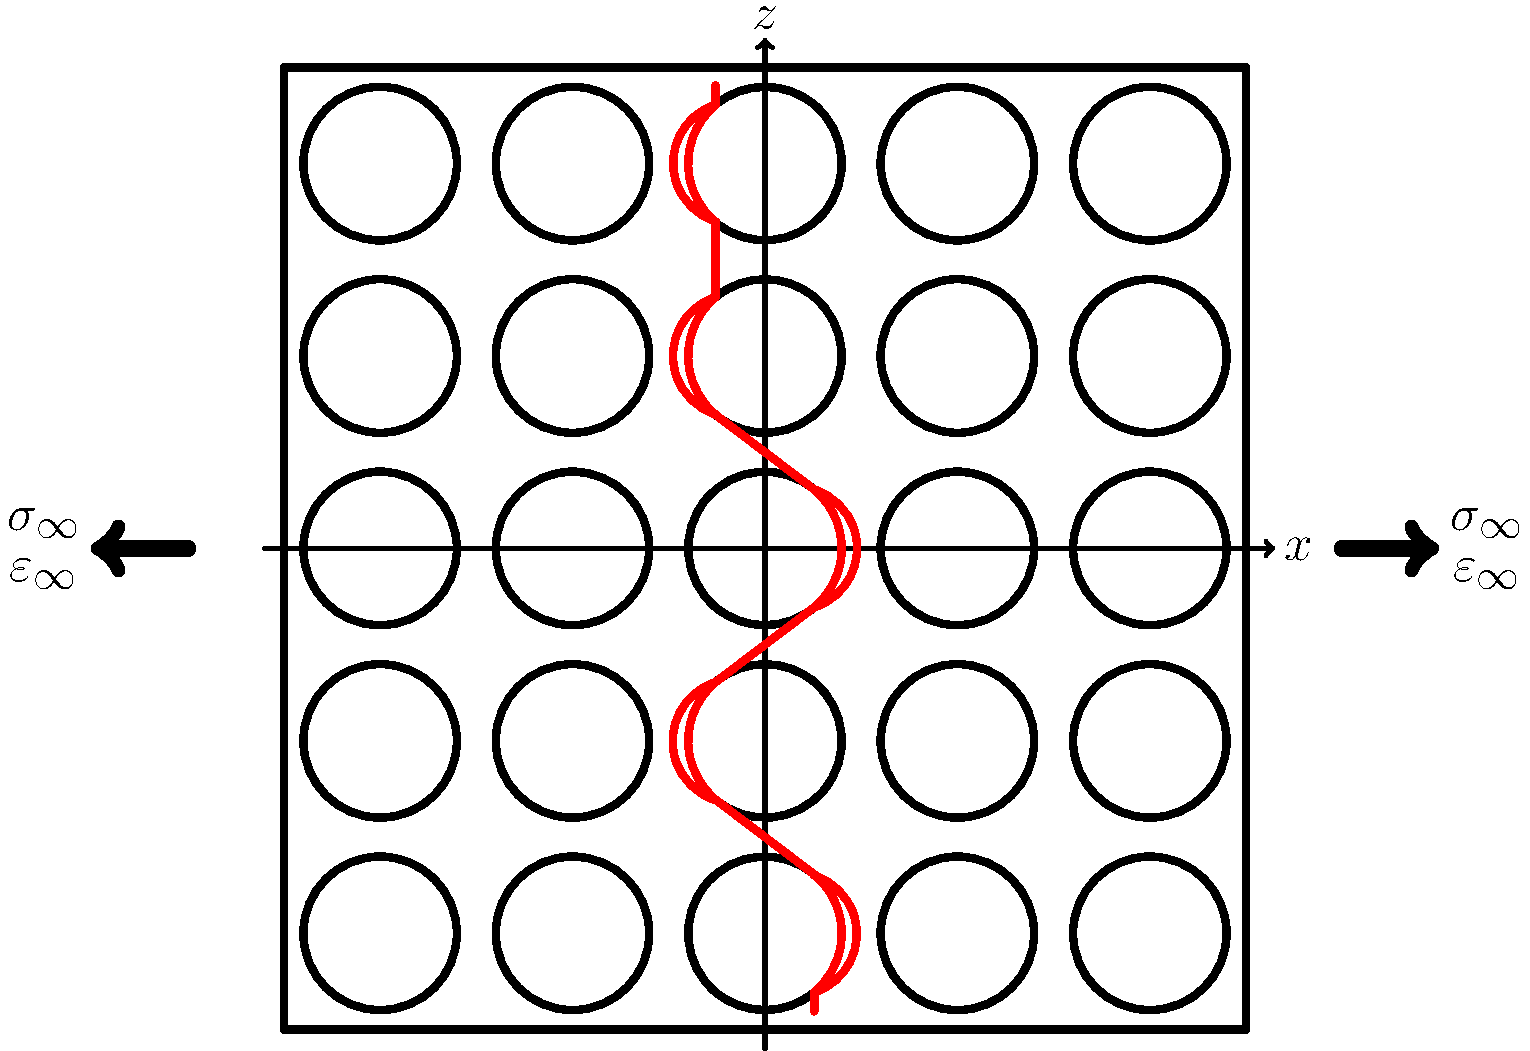
\includegraphics[width=0.6\textwidth]{stage4-coalescence.pdf}
\end{figure}
\end{alertblock}
\vspace{-0.5cm}
\pgfmathsetmacro\fontsizeref{4.5}
\pgfmathsetmacro\stretchref{1}
{\fontsize{\fontsizeref}{\stretchref} \selectfont \href{https://doi.org/10.1098/rspa.1979.0071}{Bailey et al., P. Roy. Soc. A-Math. Phy. \textbf{366} (1727), 1979.}}\\\vspace{-5pt}
{\fontsize{\fontsizeref}{\stretchref} \selectfont \href{https://doi.org/10.1007/BF00552203}{Bailey et al., J. Mater. Sci. \textbf{16} (3), 1981.}}\\\vspace{-5pt}
{\fontsize{\fontsizeref}{\stretchref} \selectfont \href{https://doi.org/10.1016/S1359-835X(96)00123-6}{Zhang et al., Compos. Part A-Appl. S. \textbf{28} (4), 1997.}}
\end{frame}


\section{Modeling}

\subsection{Geometry}

\begin{frame}
\frametitle{\vspace{0.2cm}\small Geometry}
\vspace{-1cm}
\centering
\begin{columns}[c]
\begin{column}{0.85\textwidth}
\begin{figure}
\centering
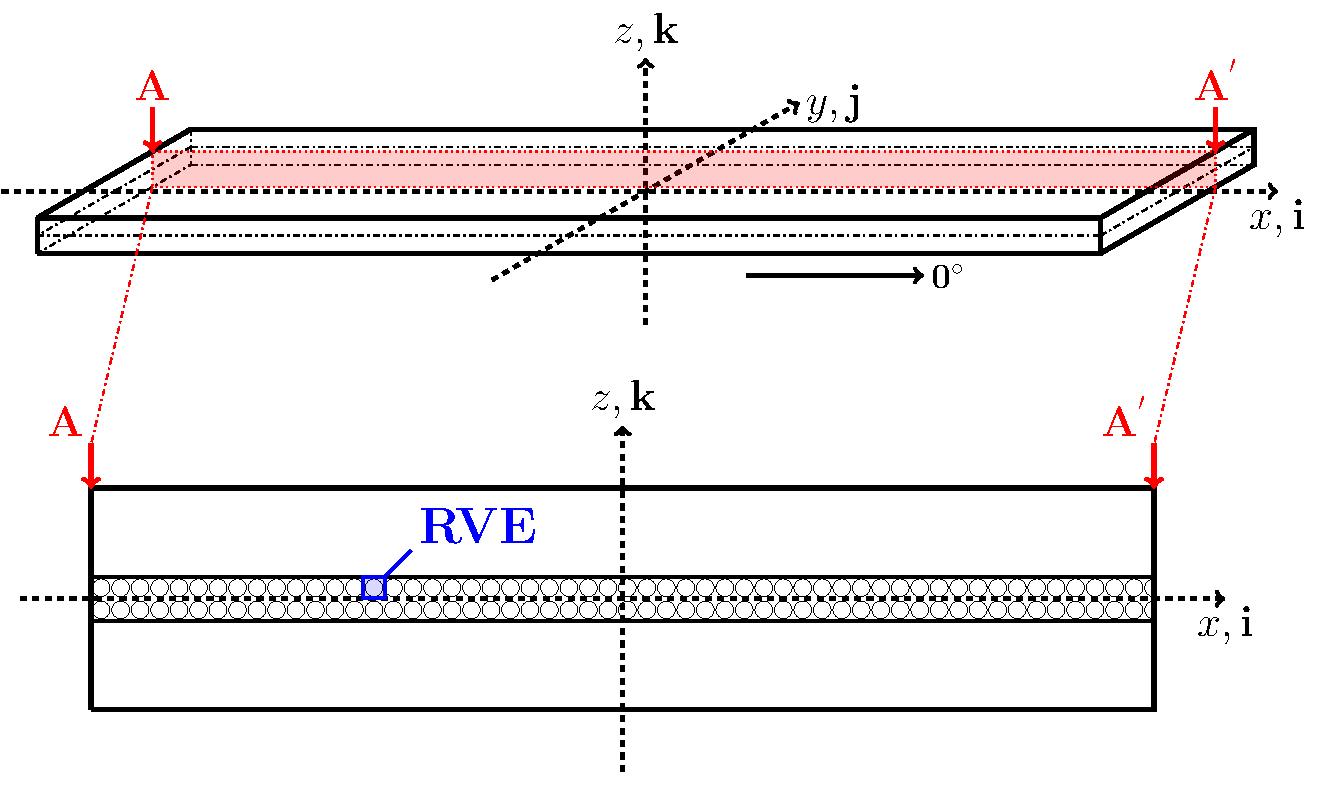
\includegraphics[width=\columnwidth]{laminate-section.pdf}
\end{figure}
\end{column}
\begin{column}{0.15\textwidth}
\scriptsize
\begin{itemize}[label=\ding{212}]
\item $L, W >> t$
\item $L, W \rightarrow \infty$
\item Square packing
\item$L_{d} >> \Delta\theta_{d}$
\item 2D RVE
\end{itemize}
\end{column}
\end{columns}
\end{frame}

\subsection{Representative Volume Elements}

\begin{frame}
\frametitle{\vspace{0.2cm}\small Representative Volume Elements}
\vspace{-1cm}
\centering
\begin{columns}[c]
\begin{column}{0.55\textwidth}
\centering
\begin{figure}
\centering
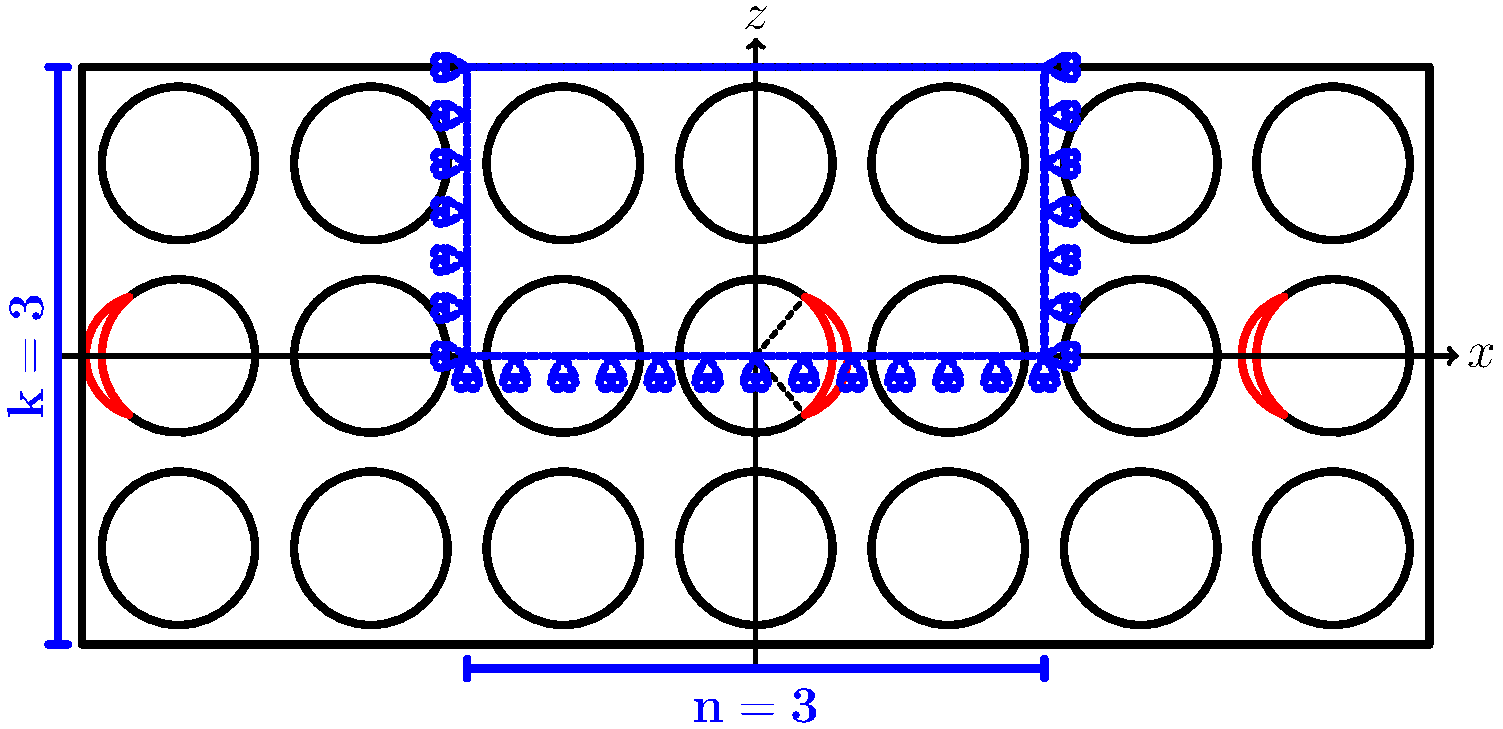
\includegraphics[width=\columnwidth]{freeThickPly.pdf}
\end{figure}
\vspace{-0.25cm}
\begin{equation*}
n\times k-free
\end{equation*}
\begin{equation*}
n\times k-H
\end{equation*}
\end{column}
\begin{column}{0.45\textwidth}
\centering
\begin{figure}
\centering
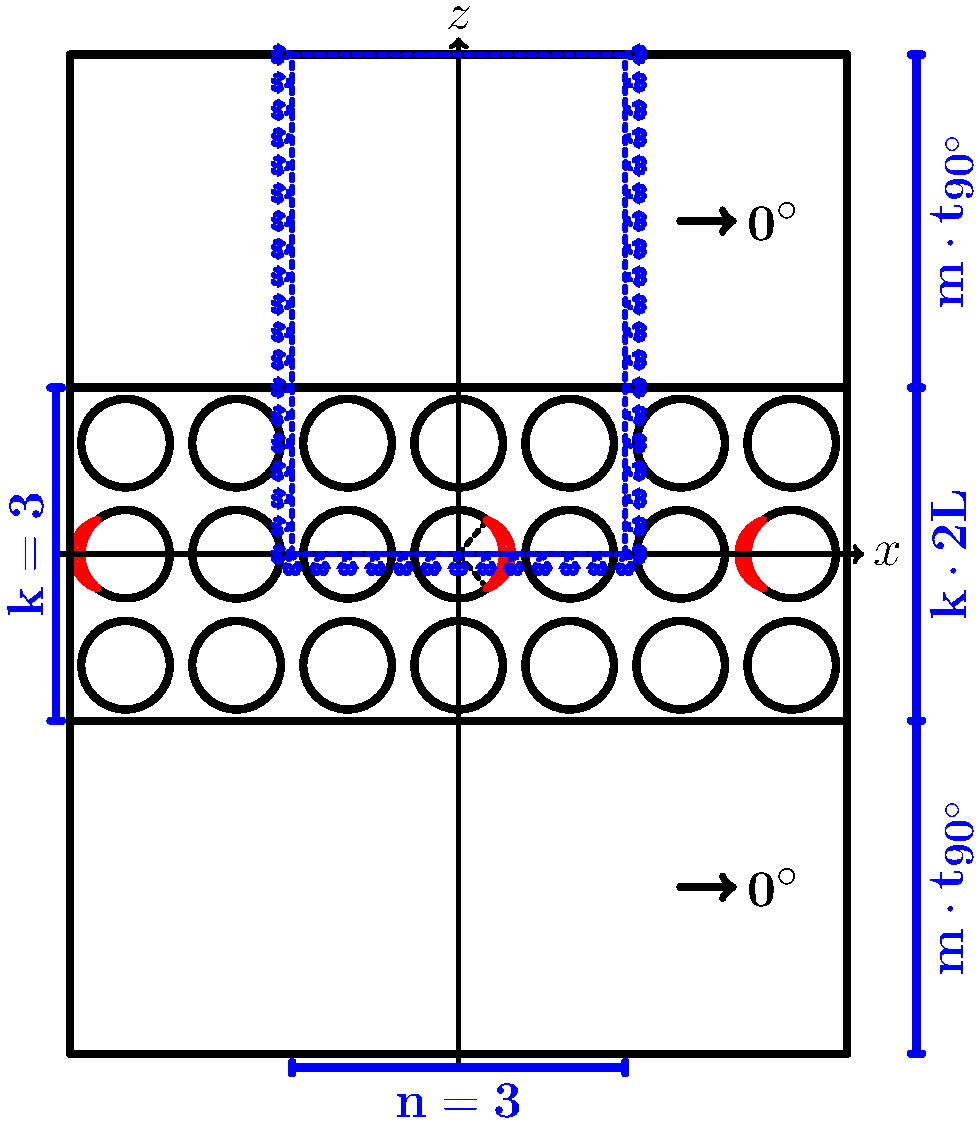
\includegraphics[width=\columnwidth]{ThickPly.pdf}
\end{figure}
\vspace{-0.25cm}
\begin{equation*}
n\times  k-m\cdot t_{90^{\circ}}
\end{equation*}
\end{column}
\end{columns}
\end{frame}

\addtocounter{framenumber}{-1}

\begin{frame}
\frametitle{\vspace{0.2cm}\small Representative Volume Elements}
\vspace{-0.9cm}
\centering
\begin{columns}[c]
\begin{column}{0.5\textwidth}
\centering
\begin{figure}
\centering
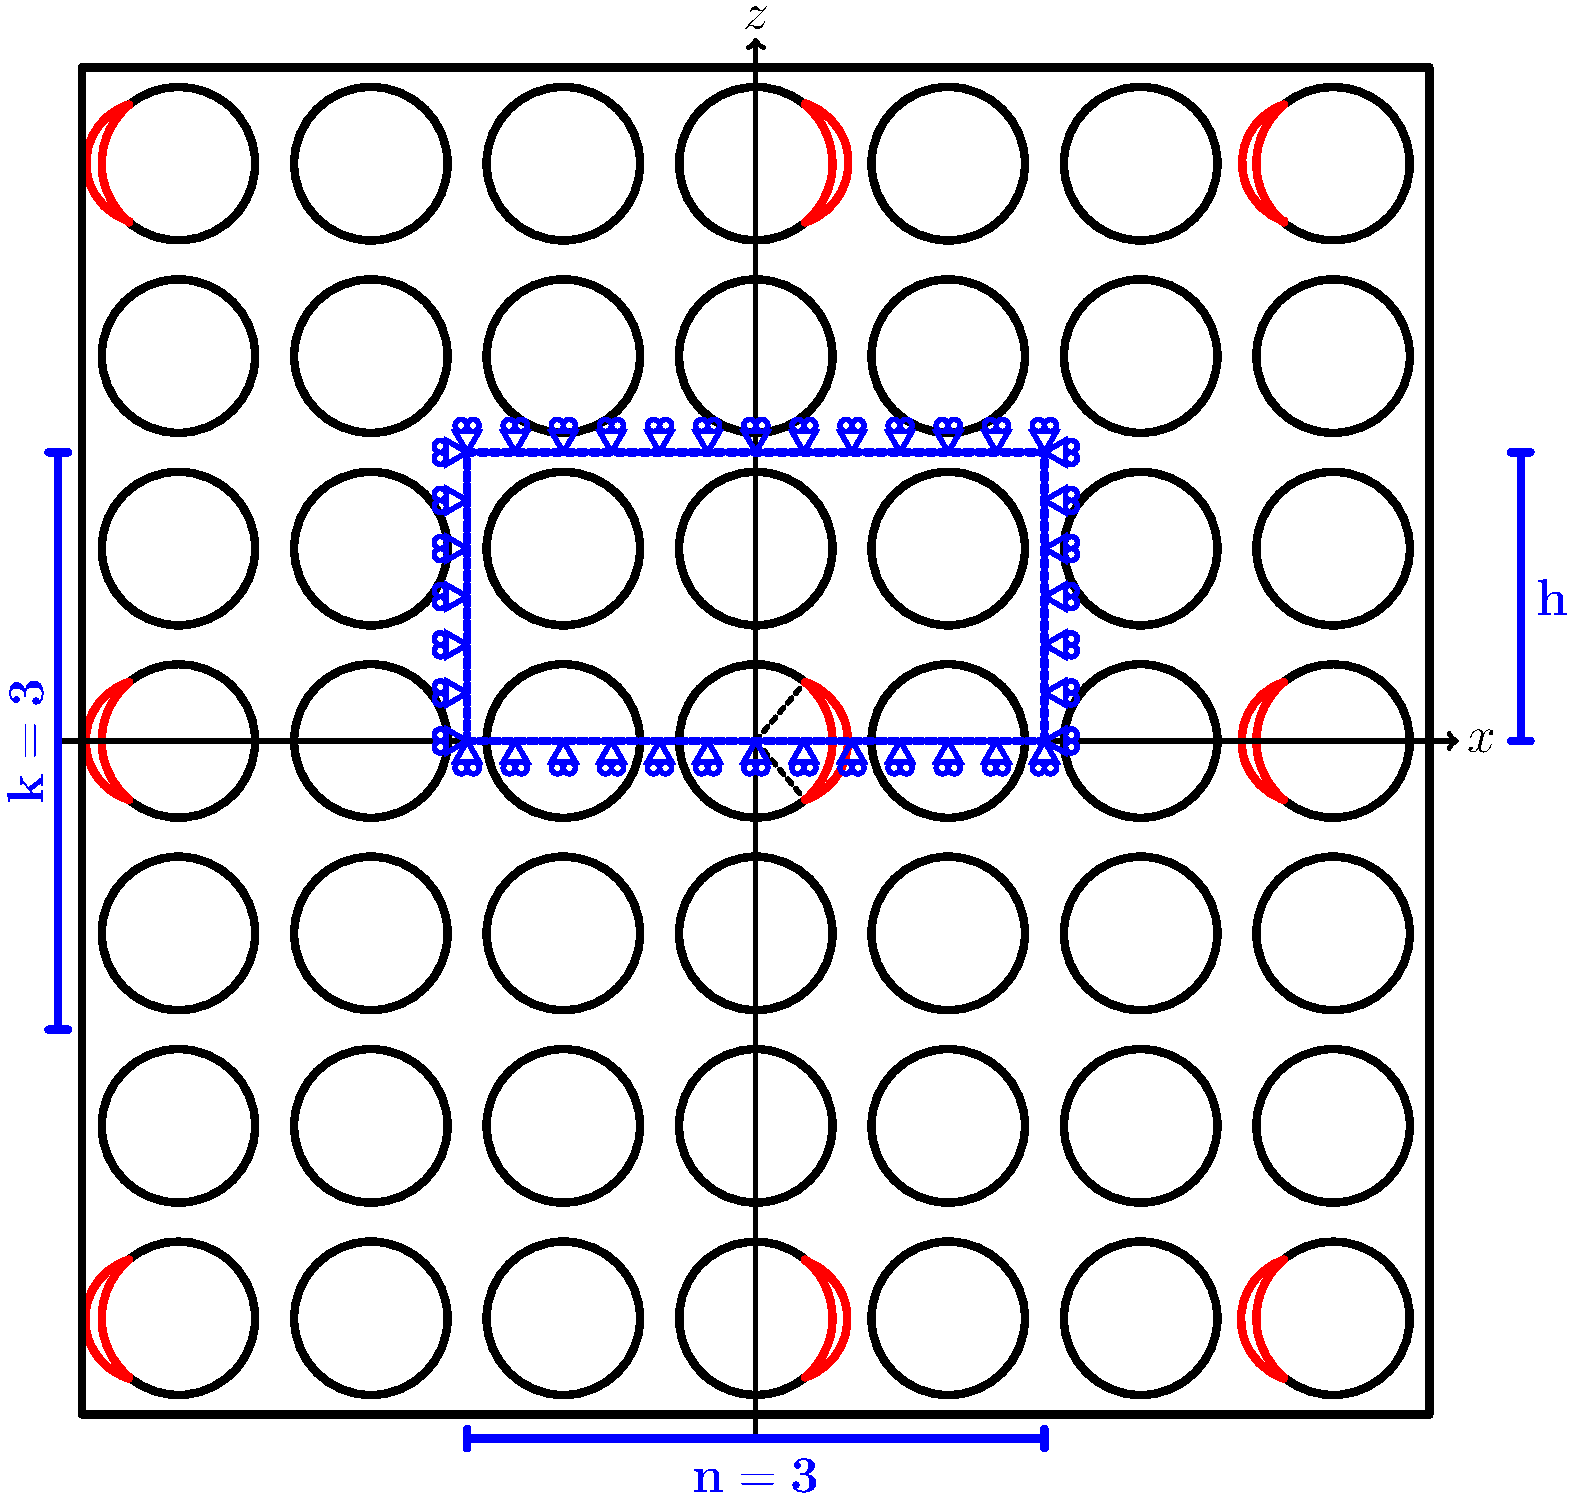
\includegraphics[width=\columnwidth]{coupling.pdf}
\end{figure}
\vspace{-0.275cm}
\begin{equation*}
\begin{split}
n\times k&-symm\ (coupling)\\
n\times k&-coupling+H
\end{split}
\end{equation*}
\end{column}
\begin{column}{0.5\textwidth}
\centering
\begin{figure}
\centering
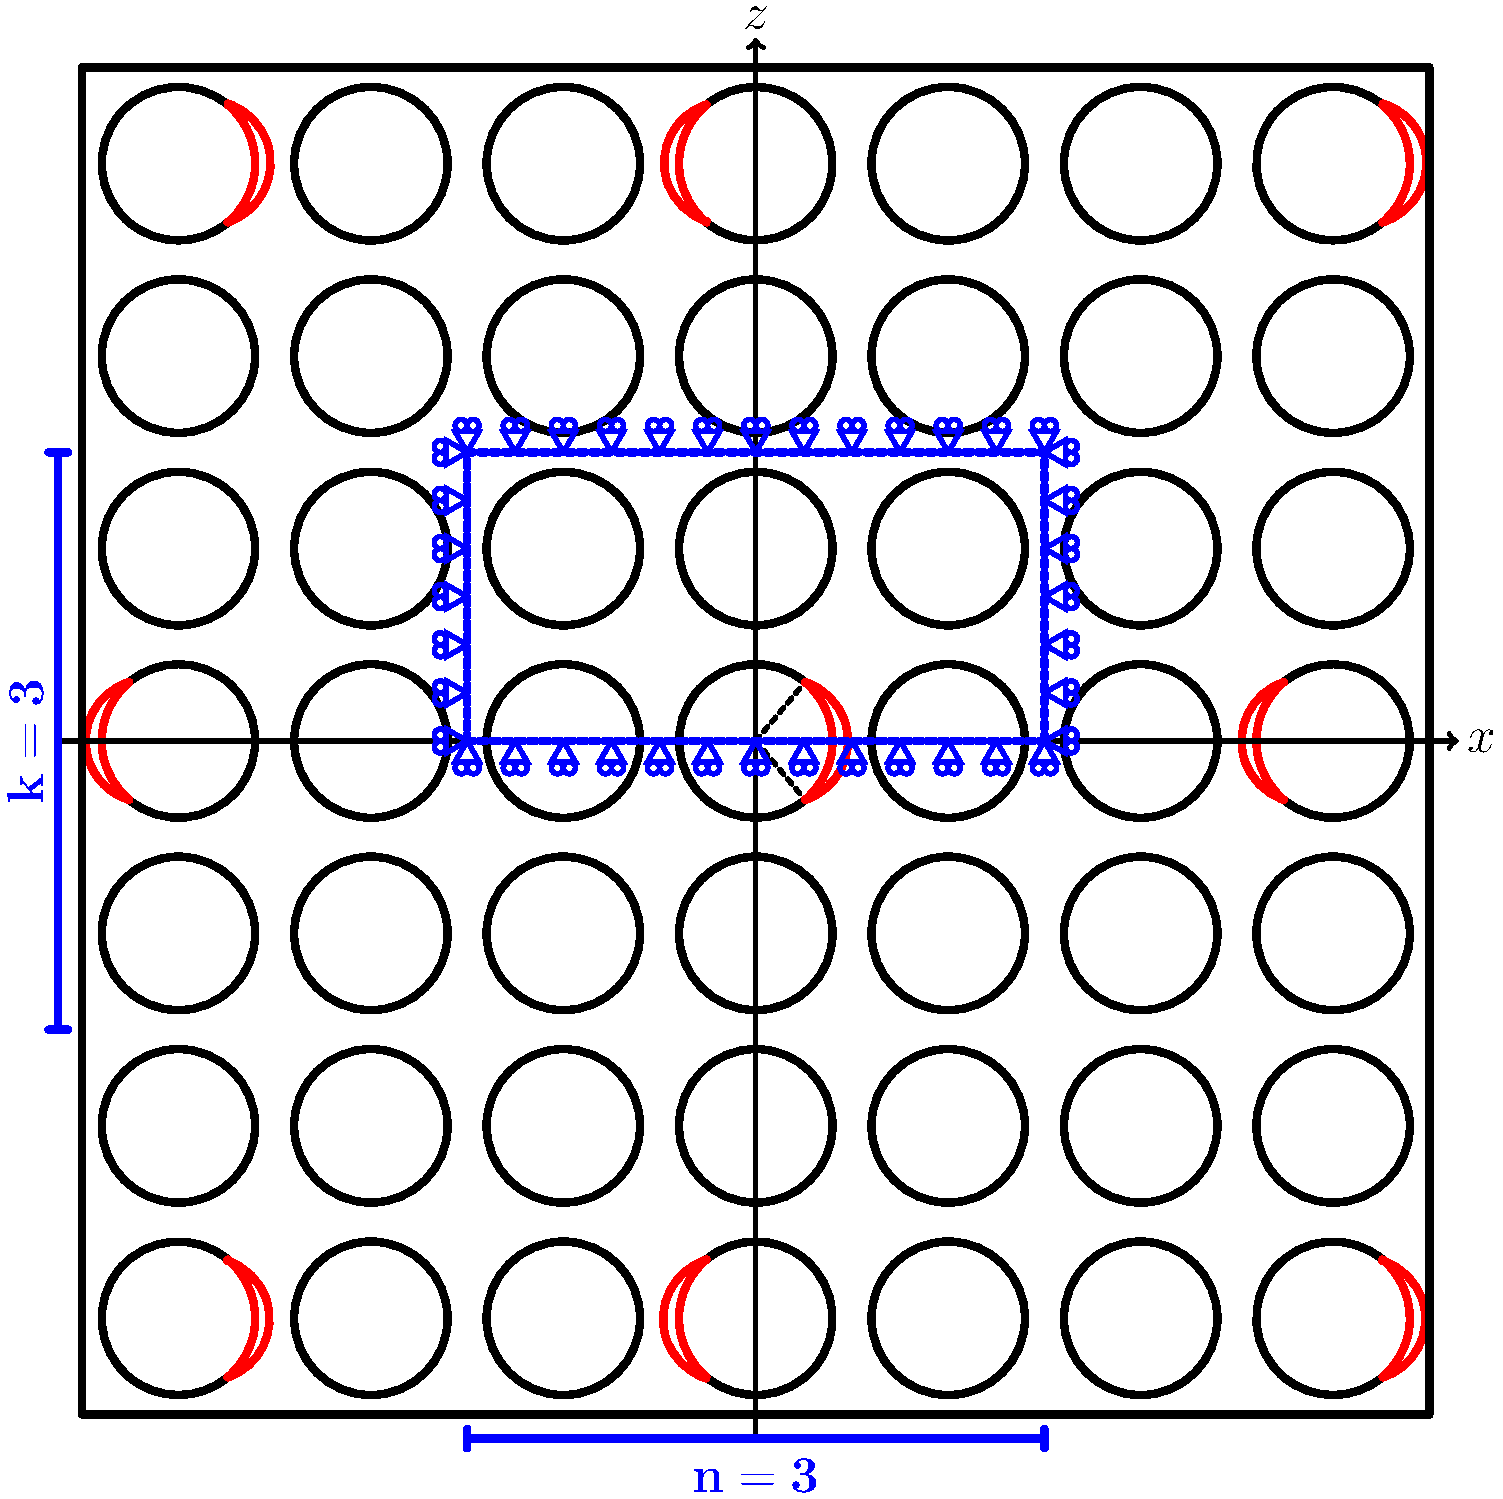
\includegraphics[width=\columnwidth]{asymm.pdf}
\end{figure}
\vspace{-0.25cm}
\begin{equation*}
n\times k-asymm
\end{equation*}
\end{column}
\end{columns}
\end{frame}

\subsection{Equivalent boundary conditions}

\begin{frame}
\frametitle{\vspace{0.2cm}\small Equivalent boundary conditions: linear horizontal displacement (H)}
\vspace{-1.25cm}
\centering
\begin{columns}[c]
\begin{column}{0.5\textwidth}
\centering
\begin{figure}
\centering
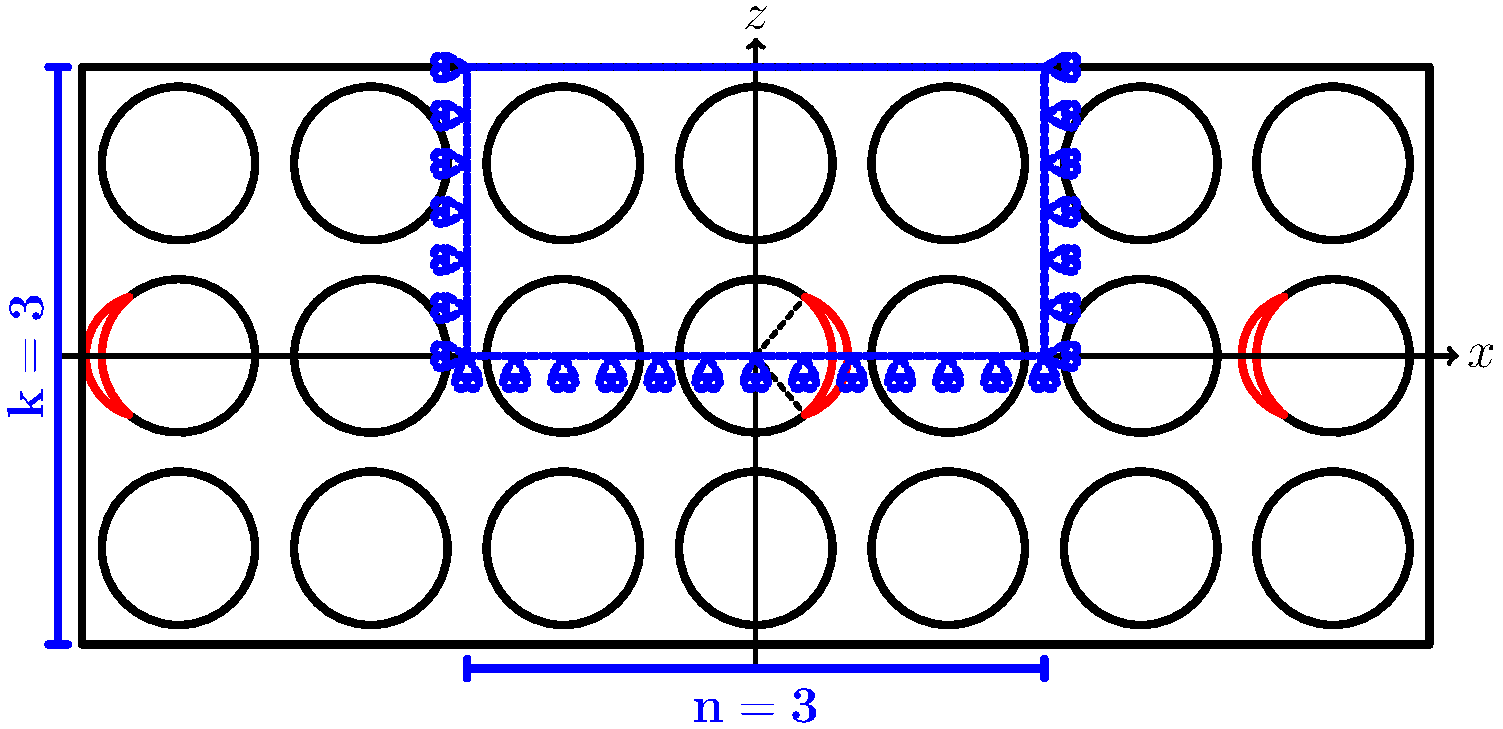
\includegraphics[width=\columnwidth]{freeThickPly.pdf}
\end{figure}
\vspace{-0.25cm}
\begin{equation*}
n\times k-H
\end{equation*}
\end{column}
\begin{column}{0.5\textwidth}
\centering
\begin{equation*}
\scriptsize
u_{x}\left(x,h\right)=\bar{\varepsilon}_{x}x
\end{equation*}
\end{column}
\end{columns}
\end{frame}

\begin{frame}
\frametitle{\vspace{0.2cm}\small Equivalent boundary conditions: symmetric coupling}
\vspace{-1.25cm}
\centering
\begin{columns}[c]
\begin{column}{0.5\textwidth}
\centering
\begin{figure}
\centering
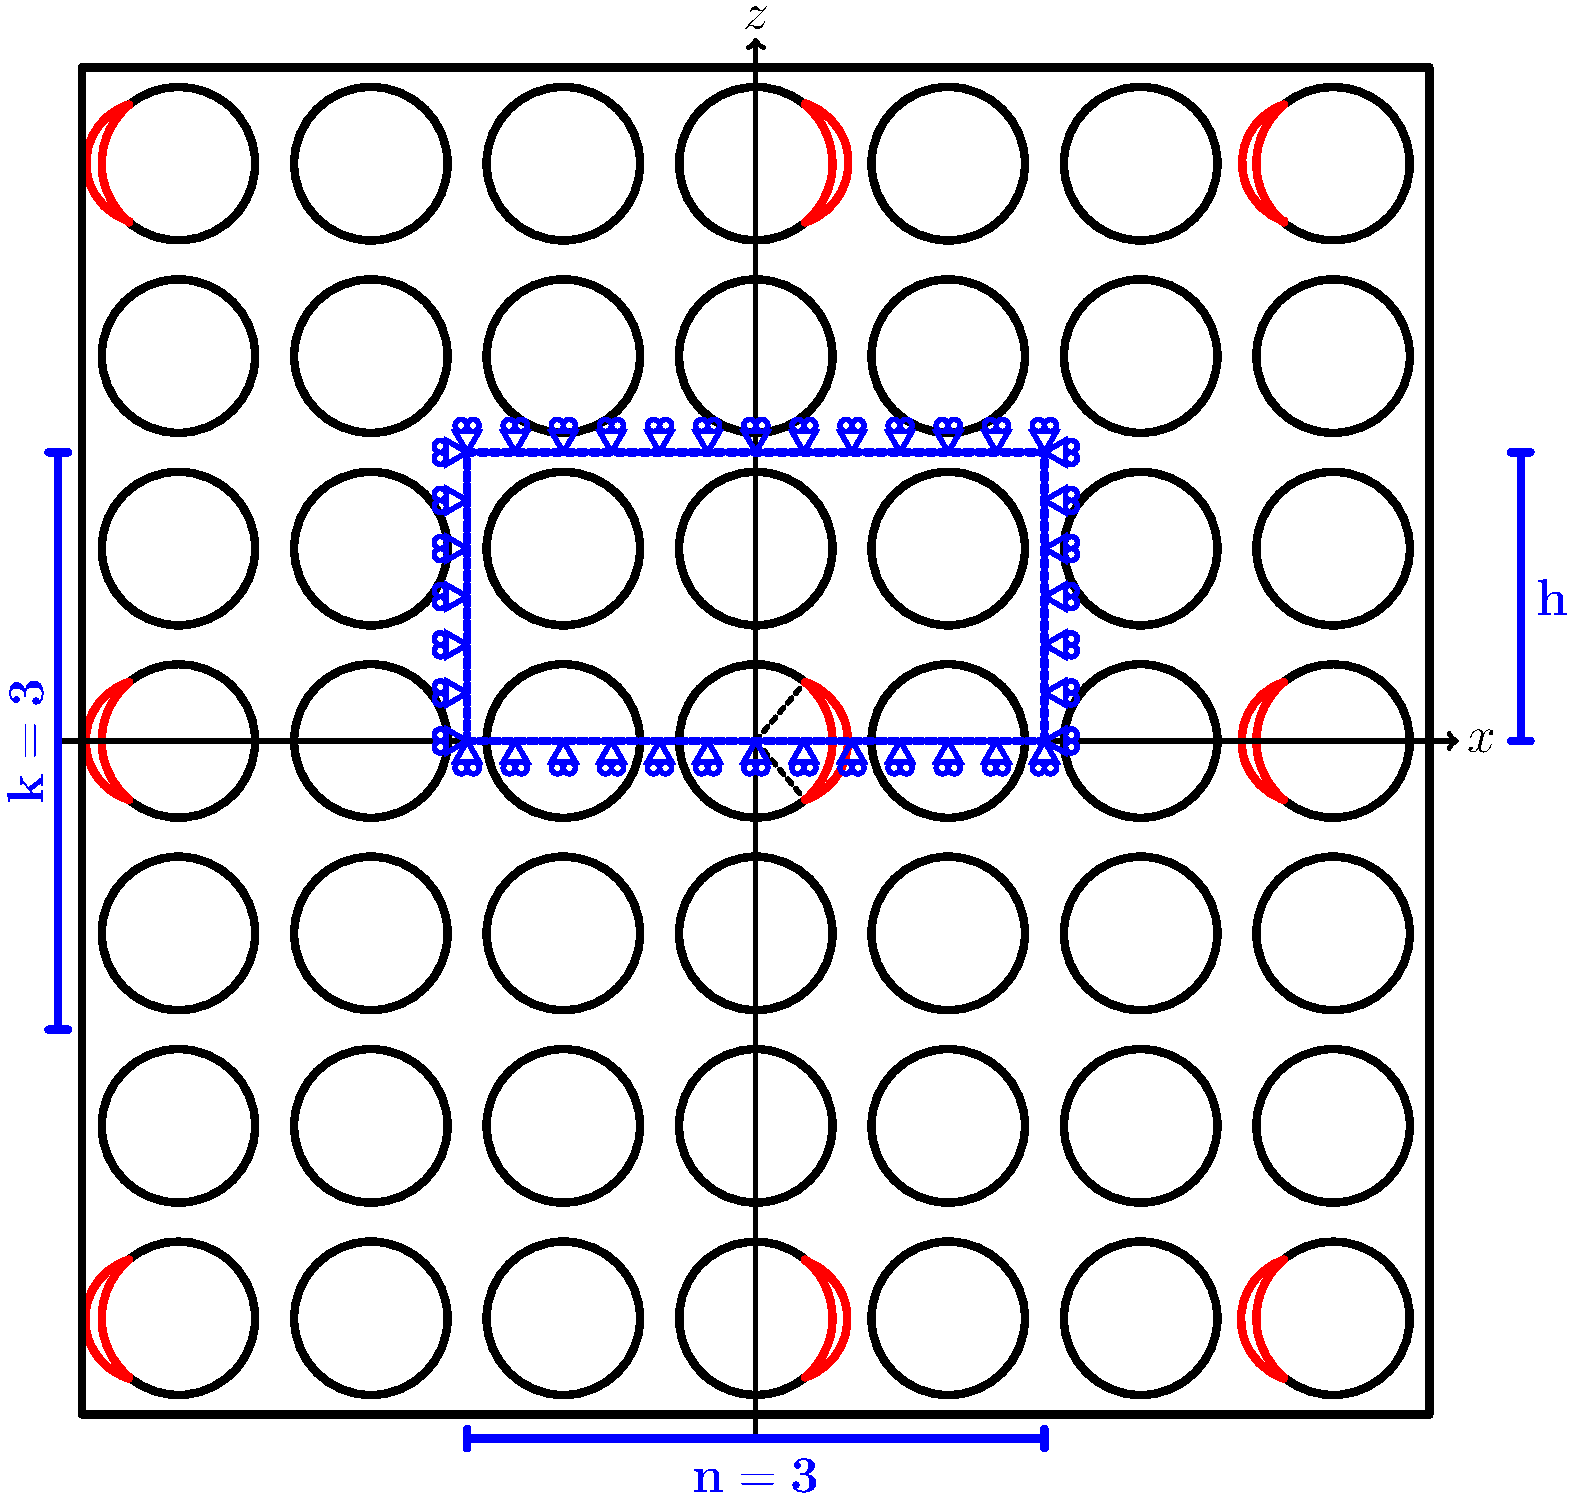
\includegraphics[width=\columnwidth]{coupling.pdf}
\end{figure}
\vspace{-0.25cm}
\begin{equation*}
n\times k-symm\ (coupling)
\end{equation*}
\end{column}
\begin{column}{0.5\textwidth}
\centering
\begin{equation*}
\scriptsize
u_{z}\left(x,h\right)=\bar{u}_{z}\left(x,h\right)
\end{equation*}
\end{column}
\end{columns}
\end{frame}

\begin{frame}
\frametitle{\vspace{0.2cm}\small Equivalent boundary conditions: coupling + H}
\vspace{-1.25cm}
\centering
\begin{columns}[c]
\begin{column}{0.5\textwidth}
\centering
\begin{figure}
\centering
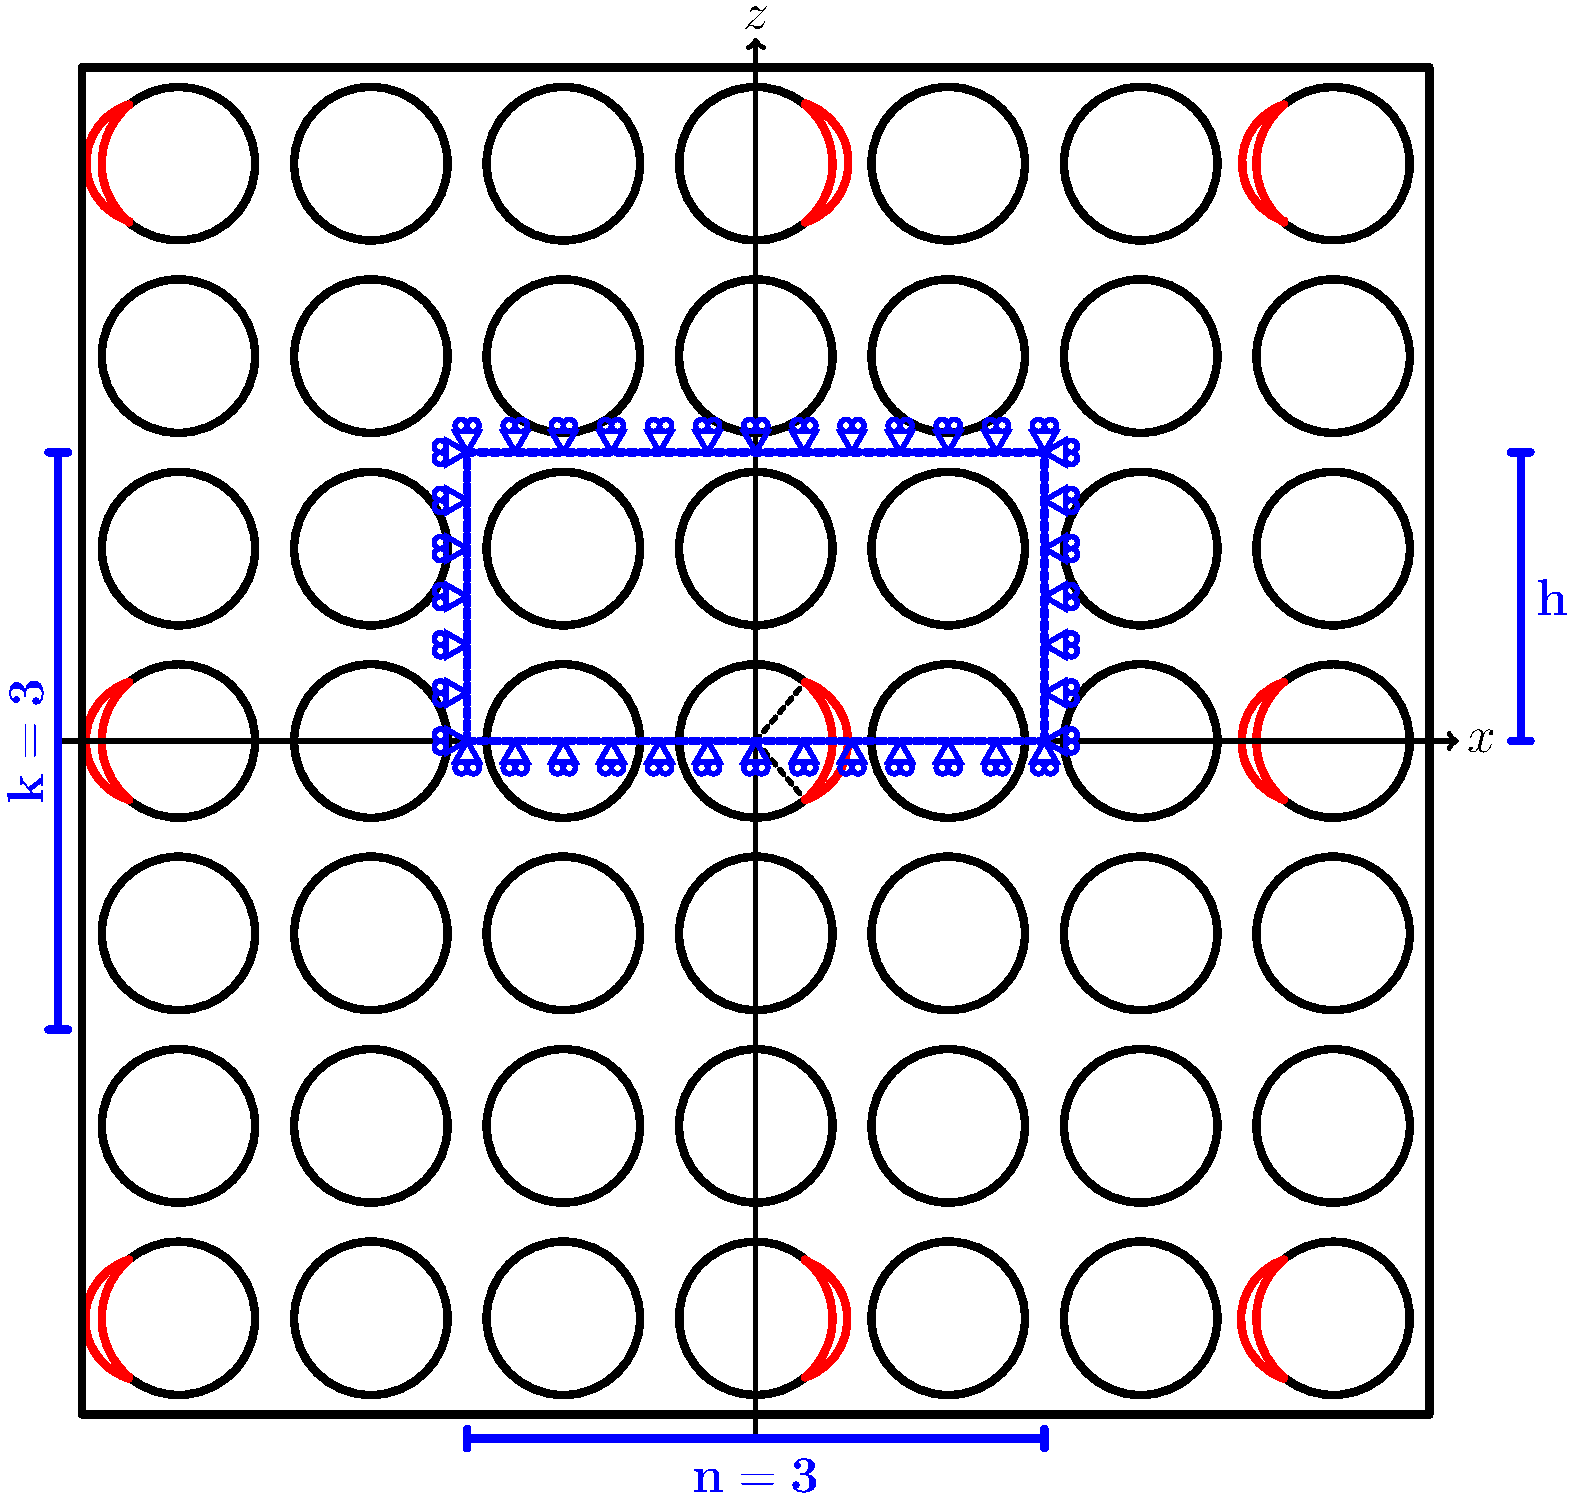
\includegraphics[width=\columnwidth]{coupling.pdf}
\end{figure}
\vspace{-0.25cm}
\begin{equation*}
n\times k-coupling+H
\end{equation*}
\end{column}
\begin{column}{0.5\textwidth}
\centering
\begin{equation*}
\scriptsize
u_{z}\left(x,h\right)=\bar{u}_{z}\left(x,h\right)
\end{equation*}
\begin{equation*}
\scriptsize
u_{x}\left(x,h\right)=\bar{\varepsilon}_{x}x
\end{equation*}
\end{column}
\end{columns}
\end{frame}

\begin{frame}
\frametitle{\vspace{0.2cm}\small Equivalent boundary conditions: anti-symmetric coupling}
\vspace{-1.25cm}
\centering
\begin{columns}[c]
\begin{column}{0.5\textwidth}
\centering
\begin{equation*}
\begin{split}
\scriptsize
u_{z}&\left(x,h\right)-u_{z}\left(0,h\right)=\\&-\left(u_{z}\left(-x,h\right)-u_{z}\left(0,h\right)\right)
\end{split}
\end{equation*}
\begin{equation*}
\scriptsize
u_{x}\left(x,h\right)=-u_{x}\left(-x,h\right)
\end{equation*}
\end{column}
\begin{column}{0.5\textwidth}
\centering
\begin{figure}
\centering
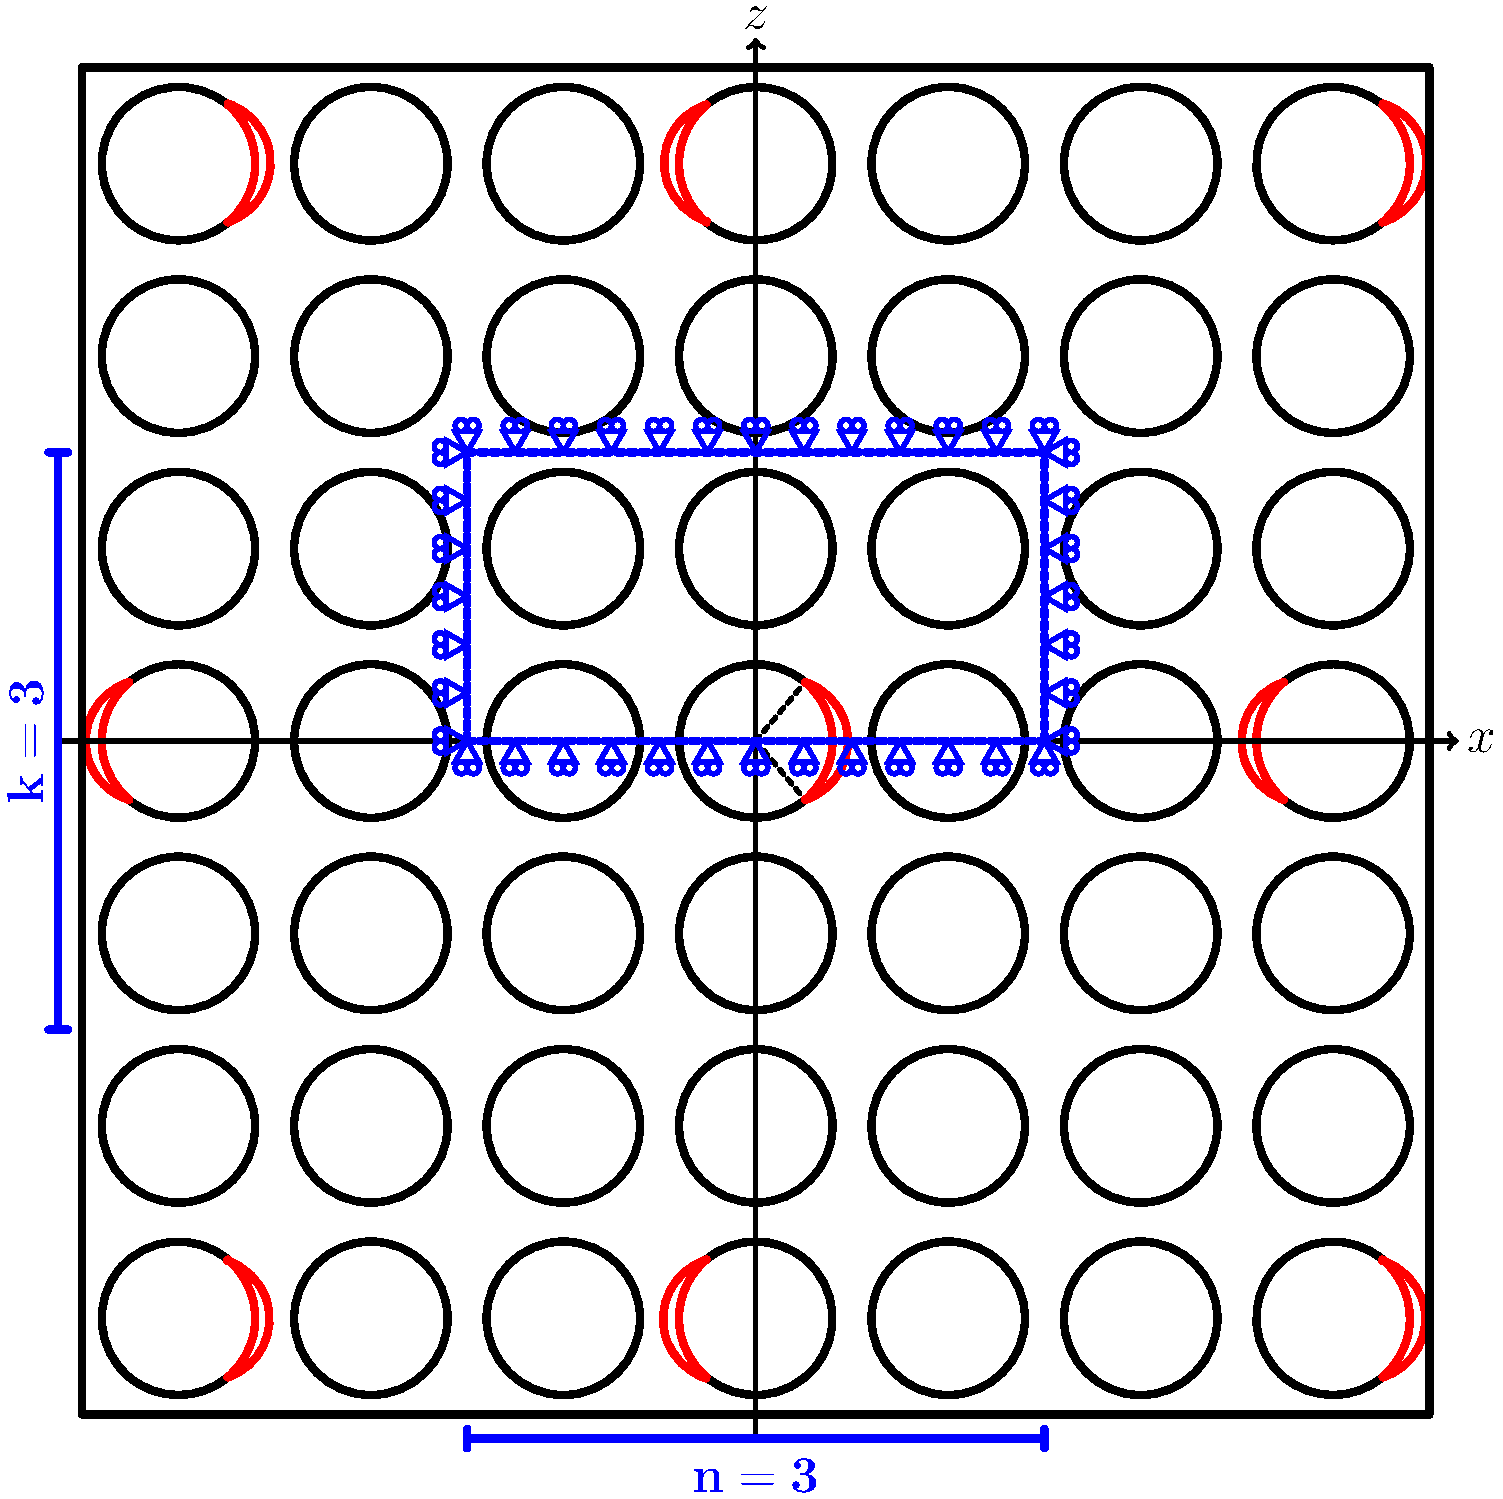
\includegraphics[width=\columnwidth]{asymm.pdf}
\end{figure}
\vspace{-0.25cm}
\begin{equation*}
n\times k-asymm
\end{equation*}
\end{column}
\end{columns}
\end{frame}

\begin{frame}
\frametitle{\vspace{0.2cm}\small Equivalent boundary conditions: validation}
\vspace{-1.25cm}
\centering
\begin{columns}[c]
\begin{column}{0.5\textwidth}
\centering
\begin{figure}
\centering
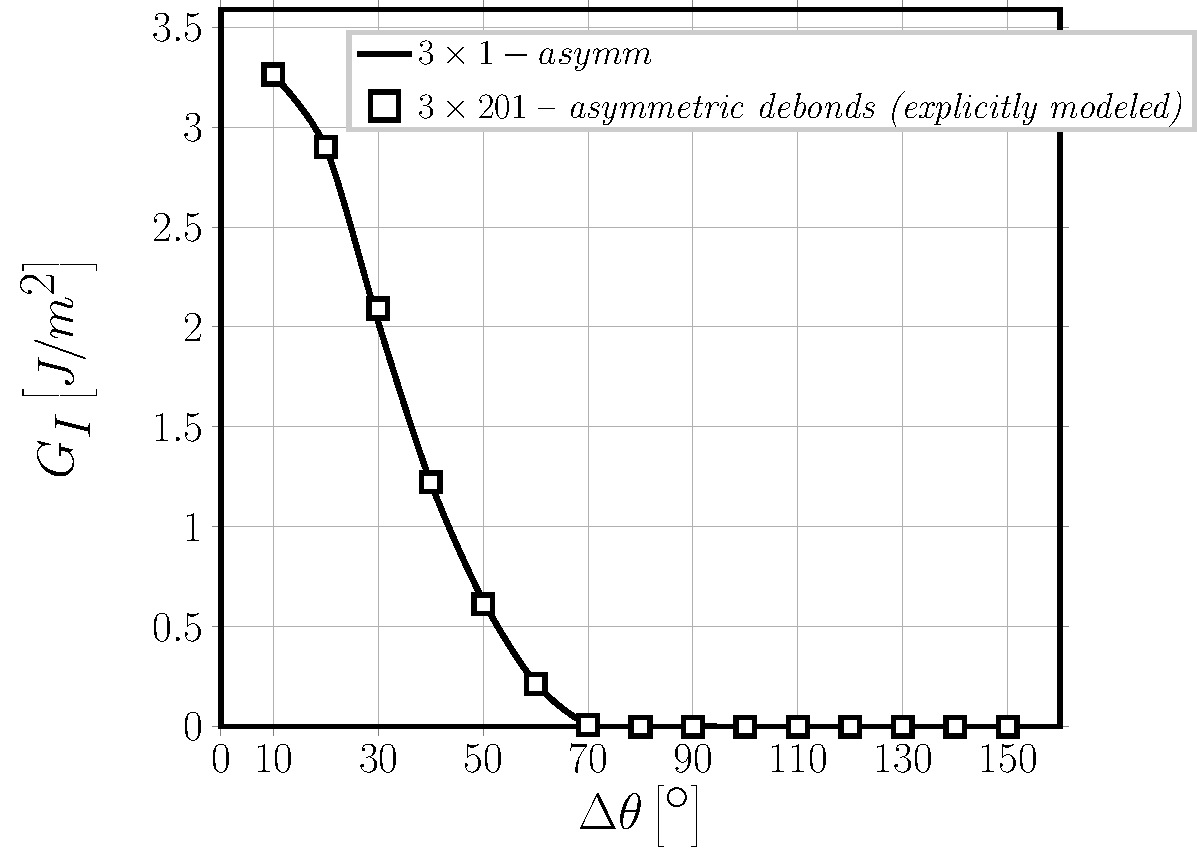
\includegraphics[width=1.1\columnwidth]{asymm-vs-explmodel-vf60-GI.pdf}
\end{figure}
\end{column}
\begin{column}{0.5\textwidth}
\centering
\begin{figure}
\centering
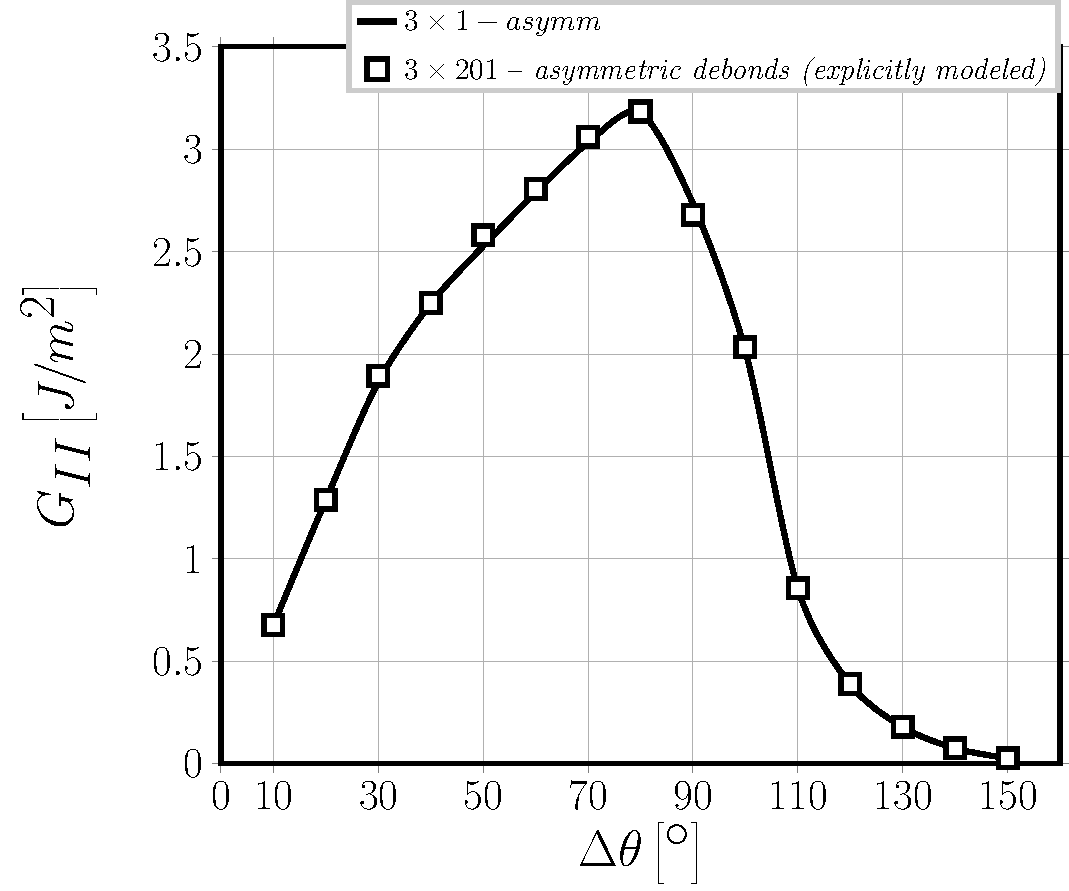
\includegraphics[width=\columnwidth]{asymm-vs-explmodel-vf60-GII.pdf}
\end{figure}
\end{column}
\end{columns}
\end{frame}

\subsection{Assumptions}

\begin{frame}
\frametitle{\vspace{0.2cm}\small Assumptions}
\vspace{-0.75cm}
\centering
\begin{columns}
\begin{column}{0.5\textwidth}
\begin{figure}
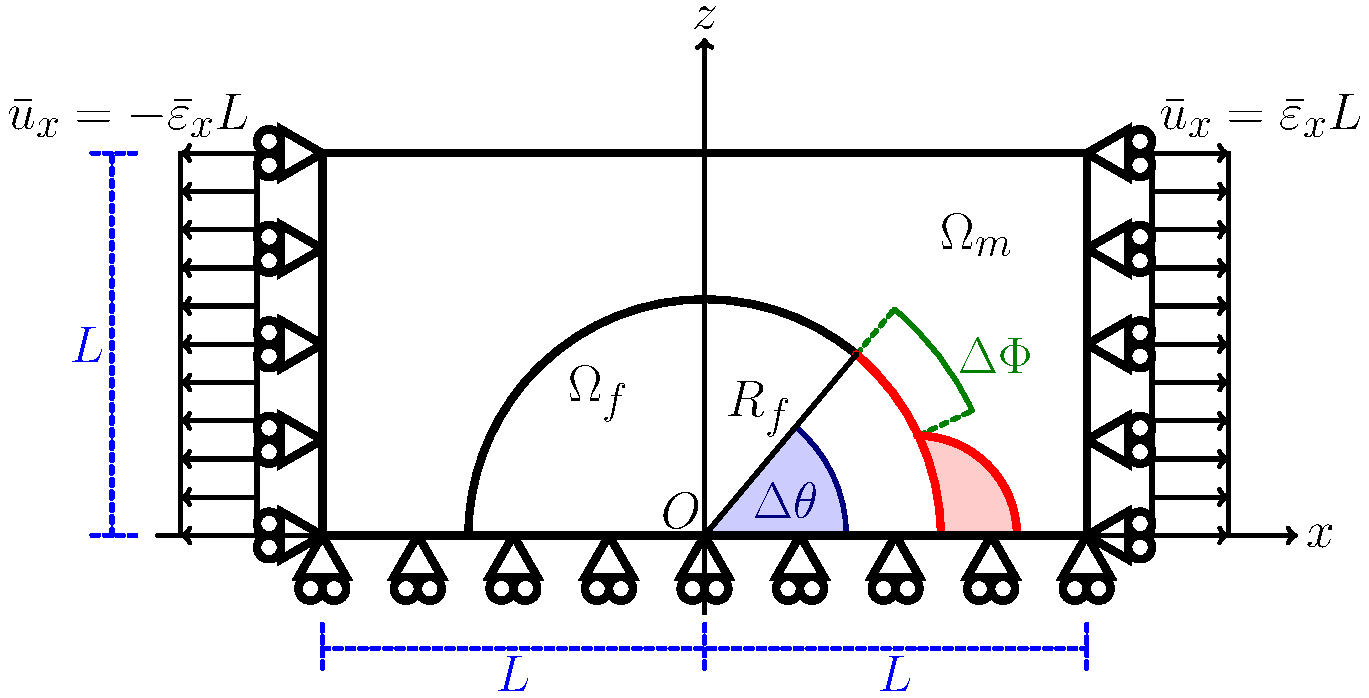
\includegraphics[width=\columnwidth]{RUC.pdf}
\end{figure}
\vspace{-0.1cm}
\tiny
\begin{equation*}
R_{f}=1\ \left[\mu m\right]\quad L=\frac{R_{f}}{2}\sqrt{\frac{\pi}{V_{f}}}
\end{equation*}
\end{column}
\begin{column}{0.5\textwidth}
\scriptsize
\begin{itemize}[label=\ding{212}]
\item Linear elastic, homogeneous materials
\item Concentric Cylinders Assembly with Self-Consistent Shear Model for UD
\item Plane strain
\item Frictionless contact interaction
\item Symmetric w.r.t. x-axis
\item Coupling of x-displacements on left and right side (repeating unit cell)
\item Applied uniaxial tensile strain $\bar{\varepsilon}_{x}=1\%$
\item $V_{f}=60\%$
\end{itemize}
\end{column}
\end{columns}
\vspace{0.05cm}
\begin{table}[htbp]
\tiny
\centering
\begin{tabular}{ccccccc}
\textbf{Material} & \textbf{$V_{f}\left[\%\right]$}\  & \textbf{$E_{L}\left[GPa\right]$}\ & \textbf{$E_{T}\left[GPa\right]$}\  & \textbf{$\mu_{LT}\left[GPa\right]$} &\textbf{$\nu_{LT}\left[-\right]$} &\textbf{$\nu_{TT}\left[-\right]$} \\
\midrule
Glass fiber &-   & 70.0 & 70.0  & 29.2 & 0.2  & 0.2\\
Epoxy    &-& 3.5 & 3.5   & 1.25 &  0.4& 0.4\\
UD&60.0&43.442&13.714& 4.315& 0.273&0.465\\
\end{tabular}
\end{table}
\end{frame}

\subsection{Solution}

\begin{frame}
\frametitle{\vspace{0.4cm}\small Solution}
\vspace{-1.1cm}
\centering
\begin{columns}
\begin{column}{0.6\textwidth}
\begin{figure}
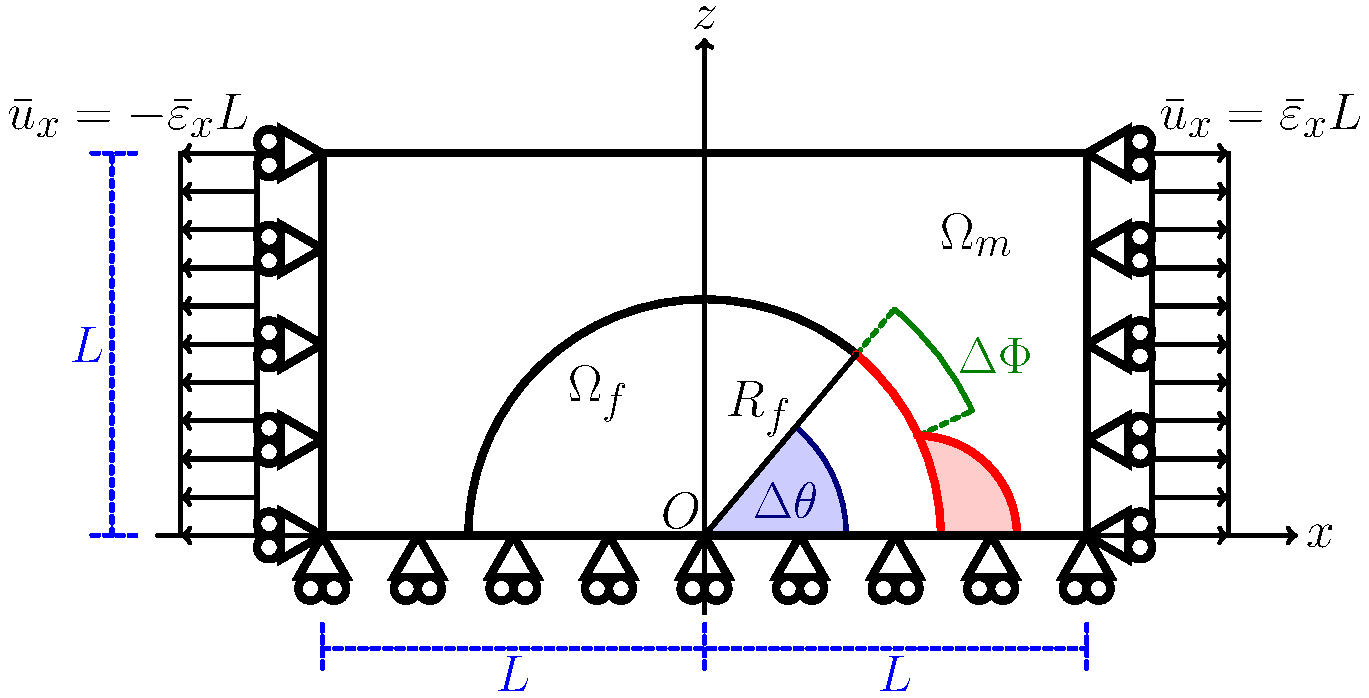
\includegraphics[width=0.825\columnwidth]{RUC.pdf}
\end{figure}
\vspace{-1cm}
\begin{columns}
\begin{column}{0.3\columnwidth}
\tiny
\begin{equation*}
\begin{aligned}
&\text{in }\Omega_{f}, \Omega_{m}, \Omega_{UD}:\\
&\frac{\partial^{2}\varepsilon_{xx}}{\partial z^{2}}+\frac{\partial^{2}\varepsilon_{zz}}{\partial x^{2}}=\frac{\partial^{2}\gamma_{zx}}{\partial x\partial z}\\
&\varepsilon_{y}=\gamma_{xy}=\gamma_{yz}=0\\
&\frac{\partial\sigma_{xx}}{\partial x}+\frac{\partial\tau_{zx}}{\partial z} = 0\\
&\frac{\partial\tau_{zx}}{\partial x}+\frac{\partial\sigma_{zz}}{\partial z} = 0\\
&\sigma_{yy}=\nu\left(\sigma_{xx}+\sigma_{zz}\right)\\
\end{aligned}
\end{equation*}
\end{column}
\begin{column}{0.7\columnwidth}
\tiny
\begin{equation*}
\begin{aligned}
&\text{for } 0^{\circ}\leq\alpha\leq\Delta\theta:\\
&\left(\overrightarrow{u}_{m}\left(R_{f},\alpha\right)-\overrightarrow{u}_{f}\left(R_{f},\alpha\right)\right)\cdot\overrightarrow{n}_{\alpha}\geq 0\\
&\text{for } \Delta\theta\leq\alpha\leq 180^{\circ}:\\
&\overrightarrow{u}_{m}\left(R_{f},\alpha\right)-\overrightarrow{u}_{f}\left(R_{f},\alpha\right)=0\\
&\sigma_{ij}=E_{ijkl}\varepsilon_{kl}\\
&+BC
\end{aligned}
\end{equation*}
\end{column}
\end{columns}
\end{column}
\begin{column}{0.375\textwidth}
\scriptsize
$\forall\ \Delta\theta\neq0^{\circ}$
\begin{itemize}[label=\ding{212}]
\item oscillating singularity
\vspace{-0.25cm}
\begin{equation*}
\sigma\sim r^{-\frac{1}{2}}\sin\left(\varepsilon\log r\right),\quad V_{f}\rightarrow 0
\end{equation*}
%\vspace{-0.25cm}
{\tiny
\begin{equation*}
\varepsilon=\frac{1}{2\pi}\log\left(\frac{1-\beta}{1+\beta}\right)
\end{equation*}
%\vspace{-0.25cm}
\begin{equation*}
\beta=\frac{\mu_{2}\left(\kappa_{1}-1\right)-\mu_{1}\left(\kappa_{2}-1\right)}{\mu_{2}\left(\kappa_{1}+1\right)+\mu_{1}\left(\kappa_{2}+1\right)}
\end{equation*}}
\item receding contact
\item $\frac{G\left(R_{f,2}\right)}{G\left(R_{f,1}\right)}=\frac{R_{f,2}}{R_{f,1}},\frac{G\left(\bar{\varepsilon}_{x,2}\right)}{G\left(\bar{\varepsilon}_{x,1}\right)}=\frac{\bar{\varepsilon}^{2}_{x,2}}{\bar{\varepsilon}^{2}_{x,1}}$
\item FEM + LEFM (VCCT)
%\item 6-nodes triangles \& 8-nodes quadrilaterals
\item regular mesh of quadrilaterals at the crack tip:
\begin{itemize}[label=-]
\item $AR\sim 1,\quad\delta=0.05^{\circ}$
%\item $\delta=0.05^{\circ}$
\end{itemize}
\end{itemize}
$\forall\ \Delta\theta$
\begin{itemize}[label=\ding{212}]
\item $2^{nd}$ order shape functions
\end{itemize}
\end{column}
\end{columns}
\end{frame}

\section{Convergence}

\subsection{$G_{TOT}$}

\begin{frame}
\frametitle{\vspace{0.25cm}\small $G_{TOT}$}
\vspace{-.75cm}
\centering
\begin{figure}
\centering
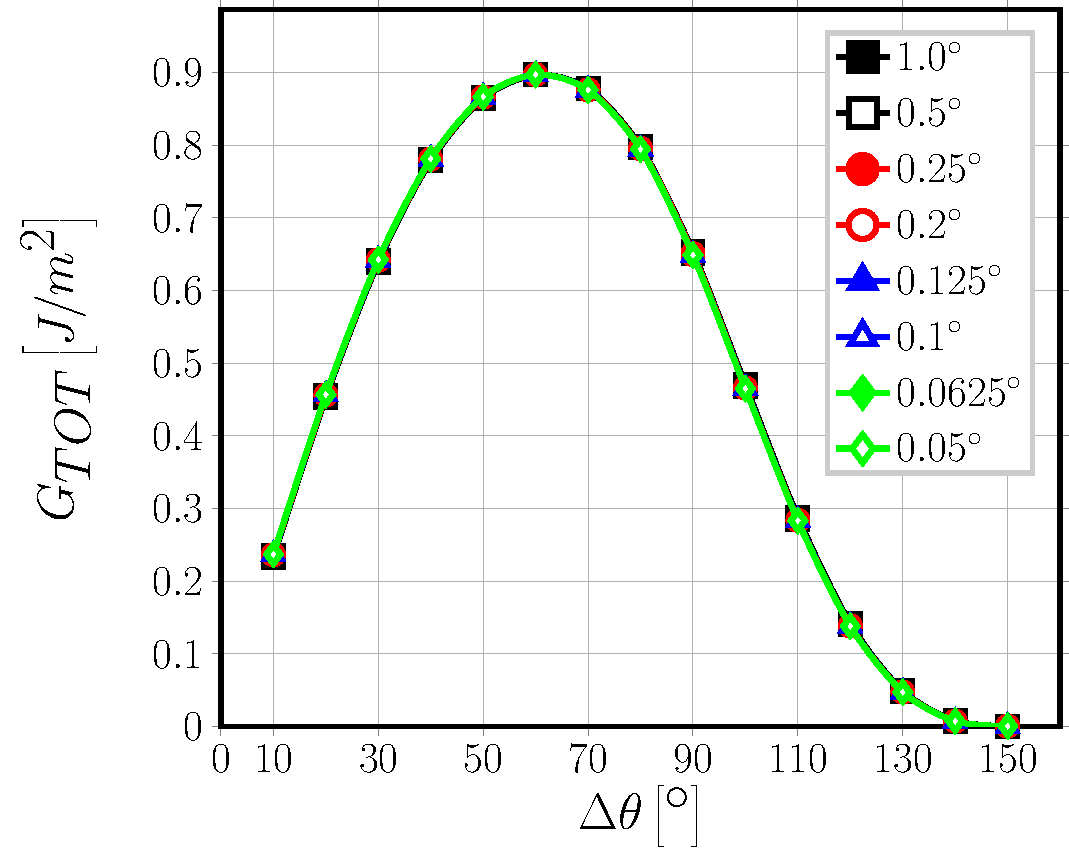
\includegraphics[width=0.6\textwidth]{Vf0_1-free-1st-GTOT.pdf}
\end{figure}
$\rightarrow 1\times1-free, V_{f}=0.1\%, 1^{st}\ order\ elements$ 
\end{frame}

\addtocounter{framenumber}{-1}

\begin{frame}
\frametitle{\vspace{0.25cm}\small $G_{TOT}$}
\vspace{-.75cm}
\centering
\begin{figure}
\centering
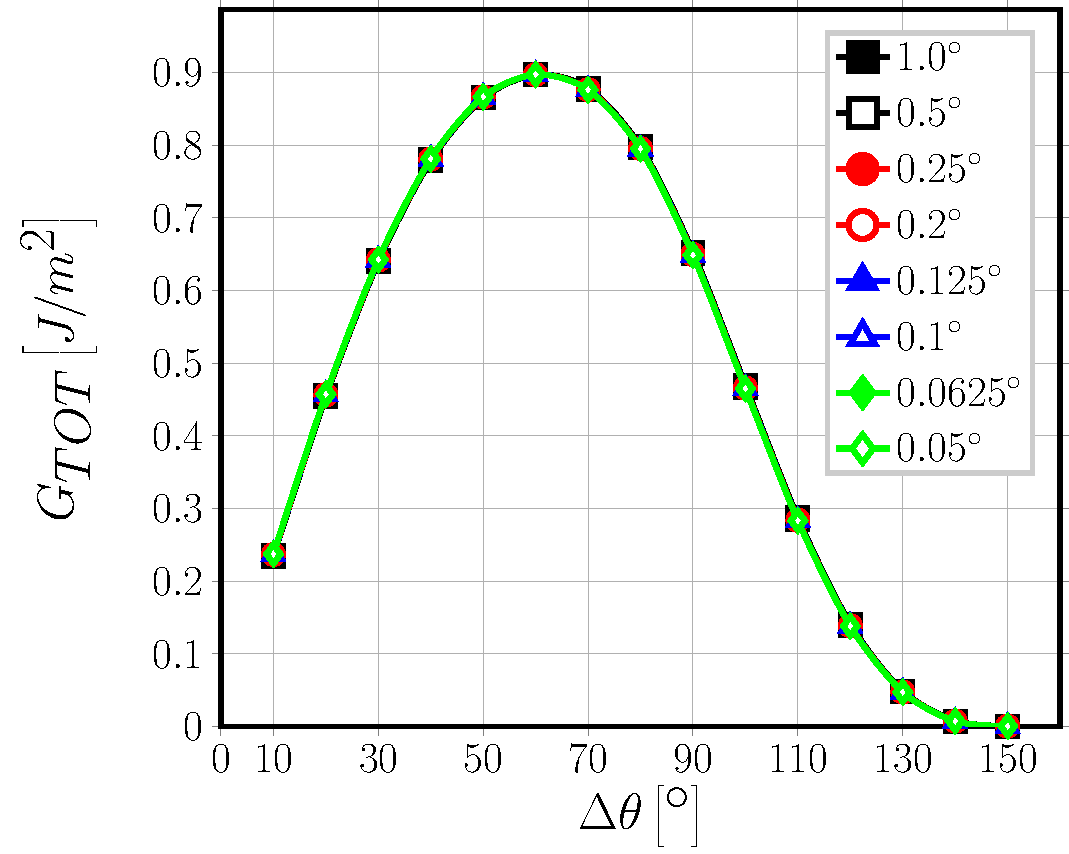
\includegraphics[width=0.6\textwidth]{Vf0_1-free-2nd-GTOT.pdf}
\end{figure}
$\rightarrow 1\times1-free, V_{f}=0.1\%, 2^{nd}\ order\ elements$ 
\end{frame}

\addtocounter{framenumber}{-1}

\begin{frame}
\frametitle{\vspace{0.25cm}\small $G_{TOT}$}
\vspace{-.75cm}
\centering
\begin{figure}
\centering
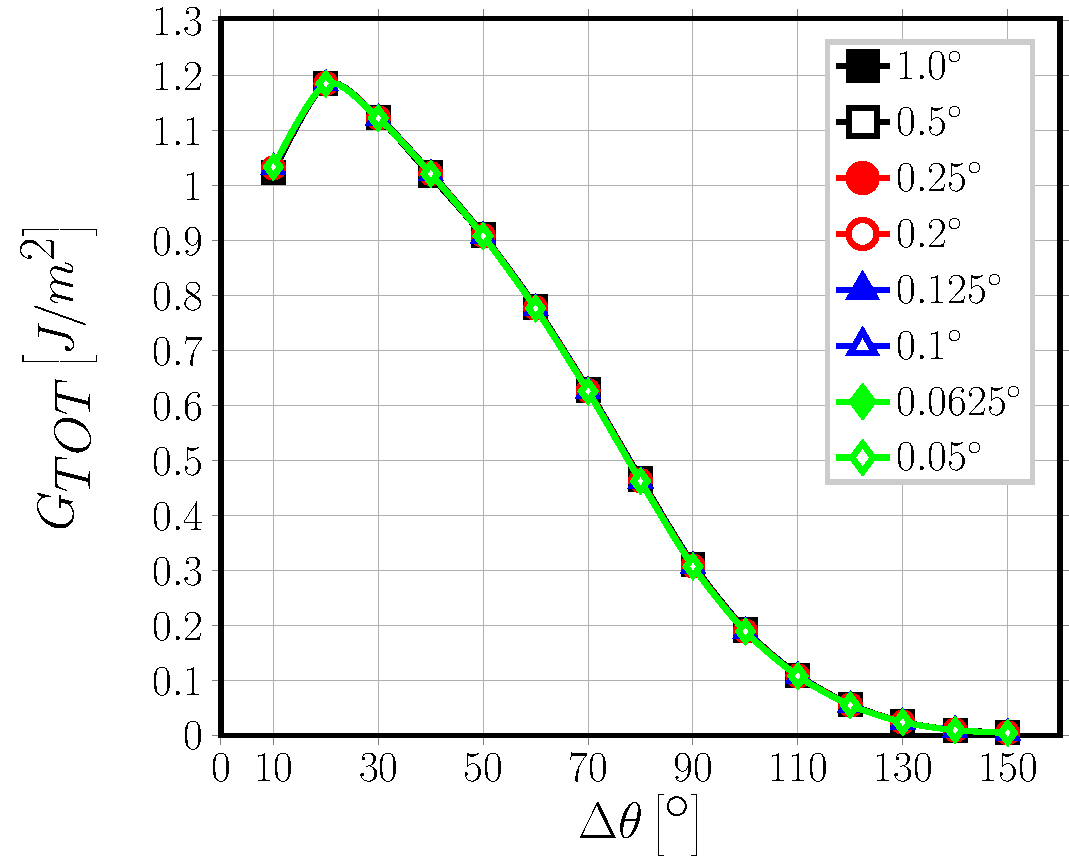
\includegraphics[width=0.6\textwidth]{Vf40-free-1st-GTOT.pdf}
\end{figure}
$\rightarrow 1\times1-free, V_{f}=40\%, 1^{st}\ order\ elements$ 
\end{frame}

\addtocounter{framenumber}{-1}

\begin{frame}
\frametitle{\vspace{0.25cm}\small $G_{TOT}$}
\vspace{-.75cm}
\centering
\begin{figure}
\centering
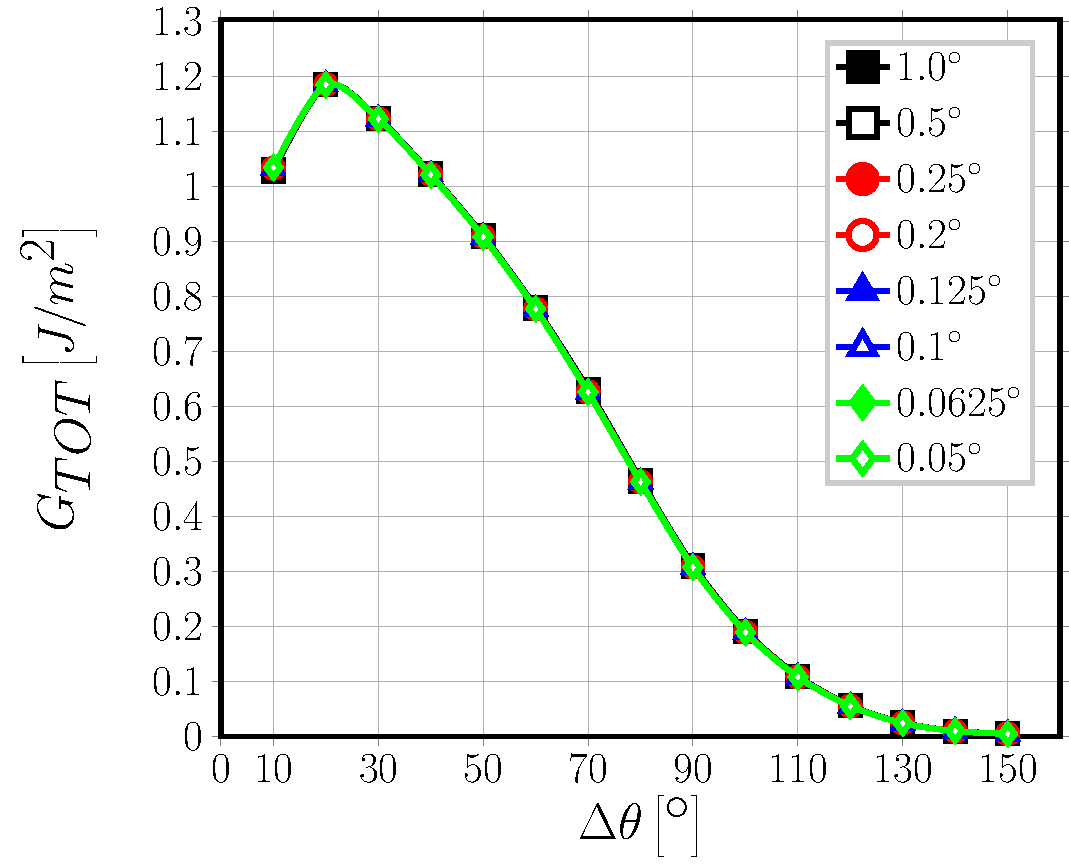
\includegraphics[width=0.6\textwidth]{Vf40-free-2nd-GTOT.pdf}
\end{figure}
$\rightarrow 1\times1-free, V_{f}=40\%, 2^{nd}\ order\ elements$ 
\end{frame}

\subsection{$G_{I}$}

\begin{frame}
\frametitle{\vspace{0.25cm}\small $G_{I}$}
\vspace{-.75cm}
\centering
\begin{figure}
\centering
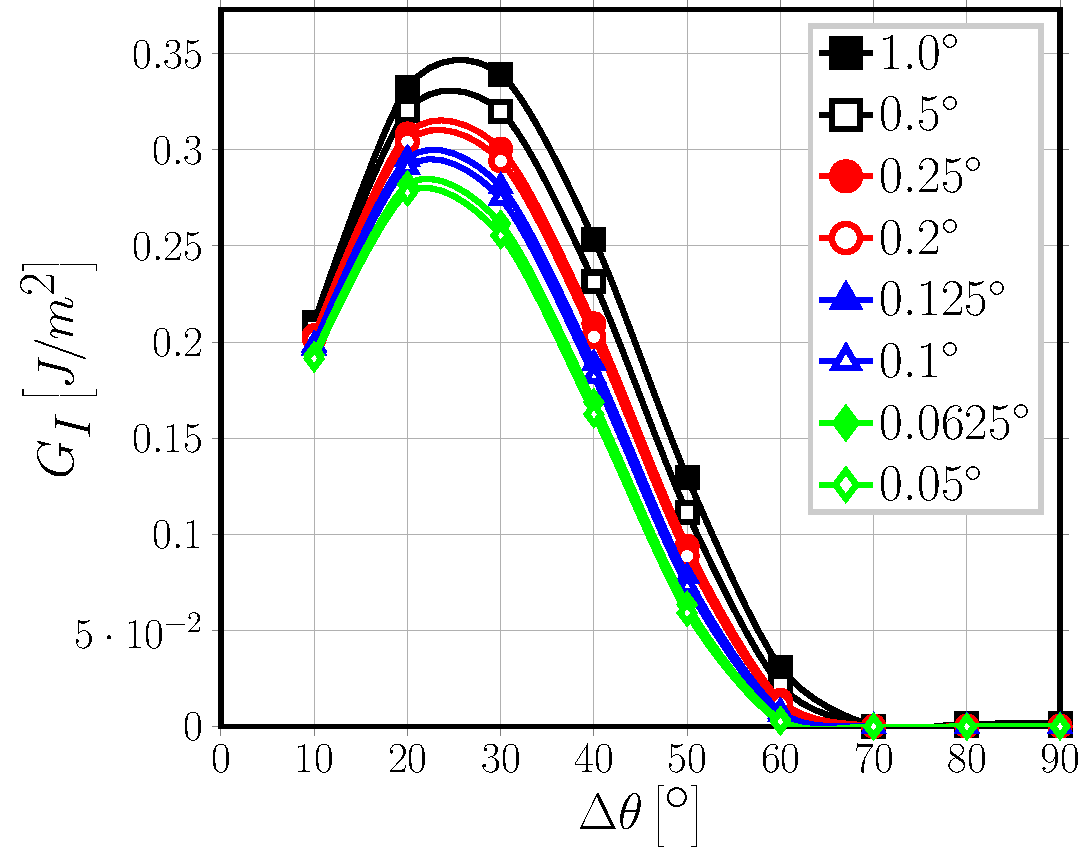
\includegraphics[width=0.6\textwidth]{Vf0_1-free-1st-GI.pdf}
\end{figure}
$\rightarrow 1\times1-free, V_{f}=0.1\%, 1^{st}\ order\ elements$ 
\end{frame}

\addtocounter{framenumber}{-1}

\begin{frame}
\frametitle{\vspace{0.25cm}\small $G_{I}$}
\vspace{-.75cm}
\centering
\begin{figure}
\centering
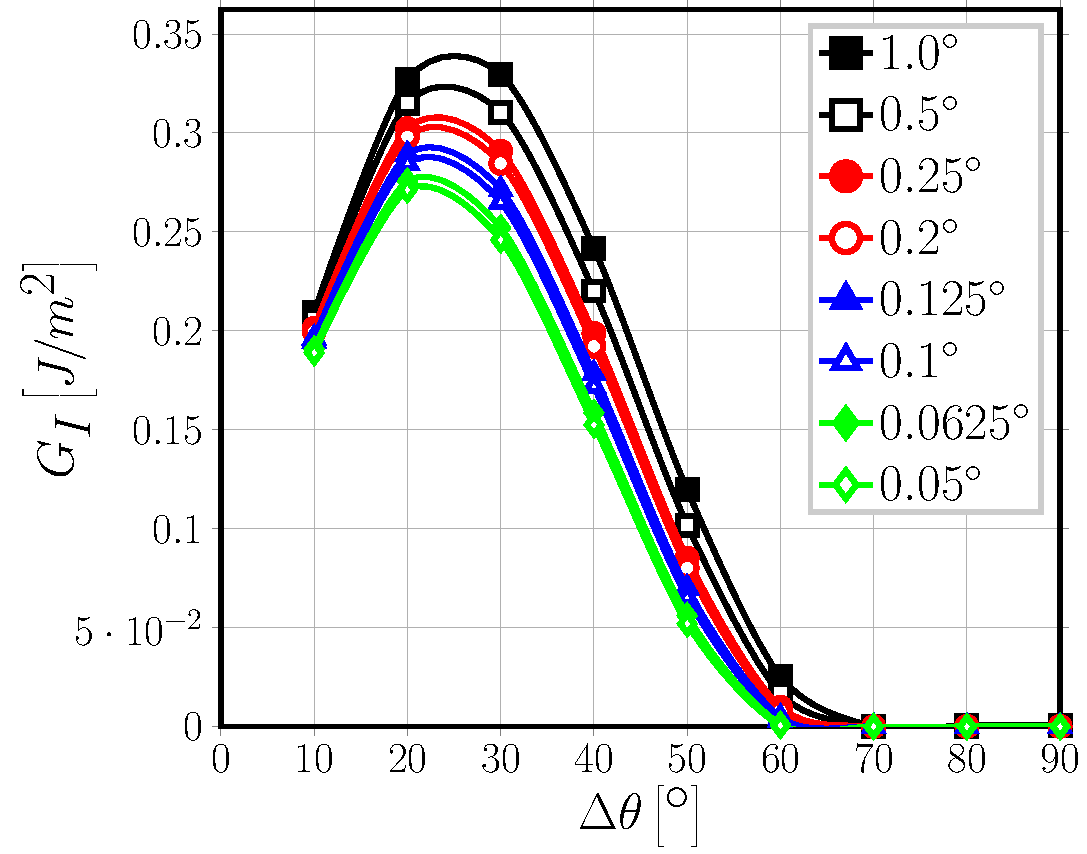
\includegraphics[width=0.6\textwidth]{Vf0_1-free-2nd-GI.pdf}
\end{figure}
$\rightarrow 1\times1-free, V_{f}=0.1\%, 2^{nd}\ order\ elements$ 
\end{frame}

\addtocounter{framenumber}{-1}

\begin{frame}
\frametitle{\vspace{0.25cm}\small $G_{I}$}
\vspace{-.75cm}
\centering
\begin{figure}
\centering
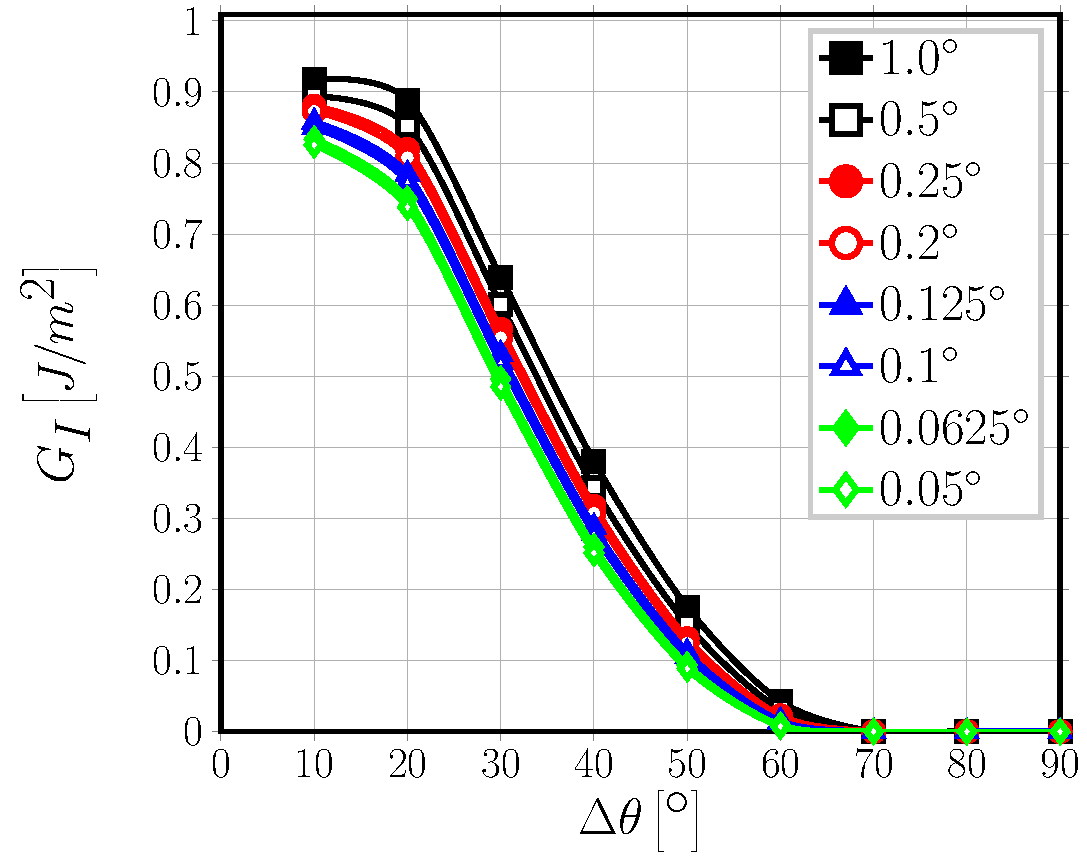
\includegraphics[width=0.6\textwidth]{Vf40-free-1st-GI.pdf}
\end{figure}
$\rightarrow 1\times1-free, V_{f}=40\%, 1^{st}\ order\ elements$ 
\end{frame}

\addtocounter{framenumber}{-1}

\begin{frame}
\frametitle{\vspace{0.25cm}\small $G_{I}$}
\vspace{-.75cm}
\centering
\begin{figure}
\centering
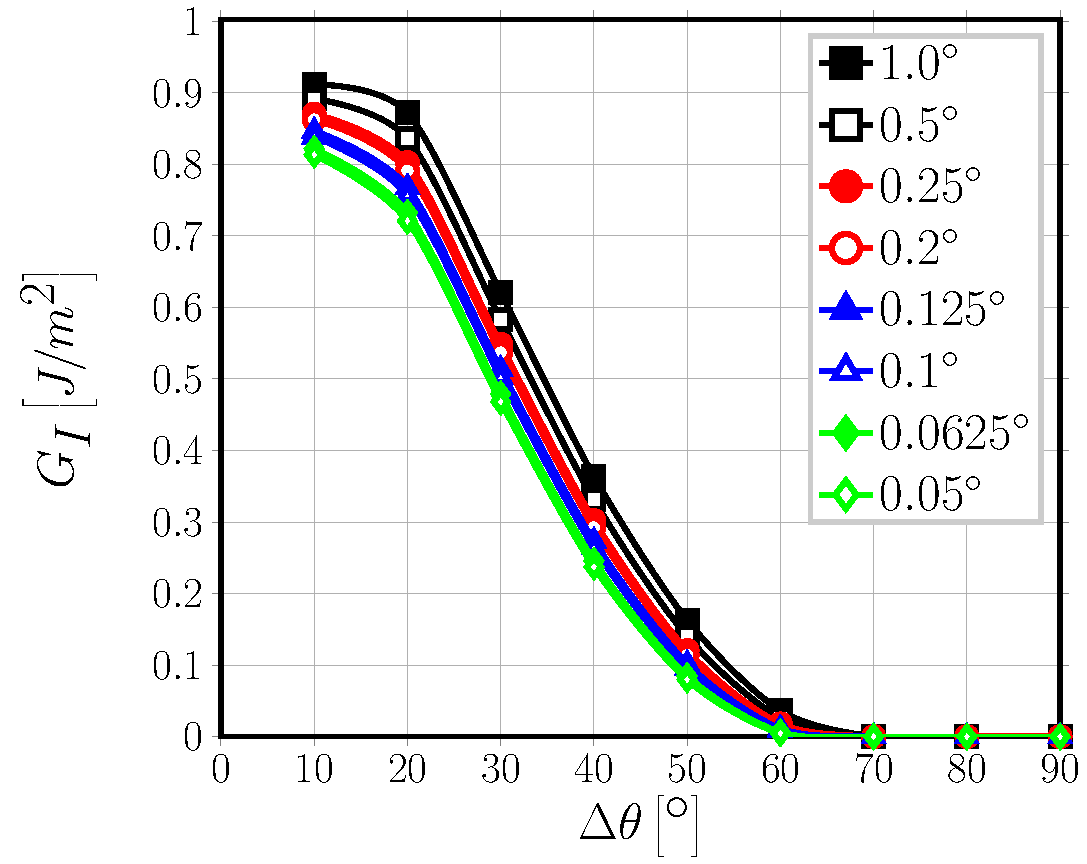
\includegraphics[width=0.6\textwidth]{Vf40-free-2nd-GI.pdf}
\end{figure}
$\rightarrow 1\times1-free, V_{f}=40\%, 2^{nd}\ order\ elements$ 
\end{frame}

\subsection{$G_{II}$}

\begin{frame}
\frametitle{\vspace{0.25cm}\small $G_{II}$}
\vspace{-.75cm}
\centering
\begin{figure}
\centering
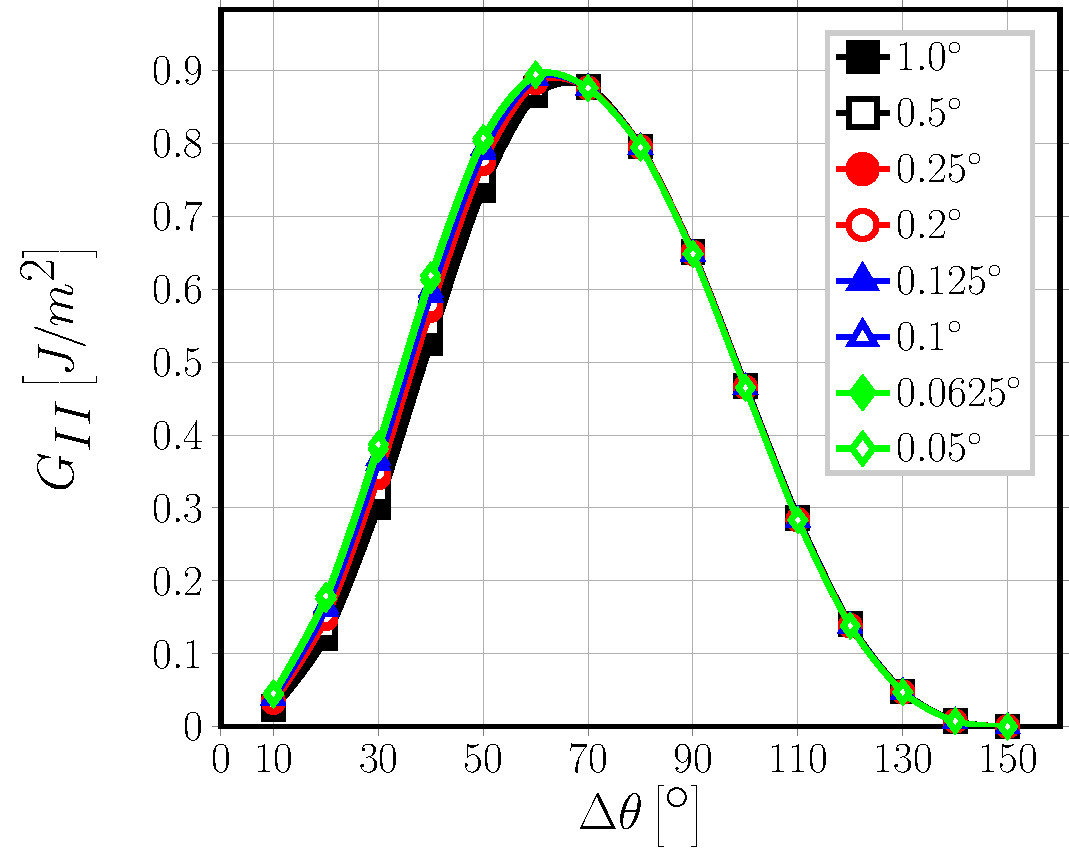
\includegraphics[width=0.6\textwidth]{Vf0_1-free-1st-GII.pdf}
\end{figure}
$\rightarrow 1\times1-free, V_{f}=0.1\%, 1^{st}\ order\ elements$ 
\end{frame}

\addtocounter{framenumber}{-1}

\begin{frame}
\frametitle{\vspace{0.25cm}\small $G_{II}$}
\vspace{-.75cm}
\centering
\begin{figure}
\centering
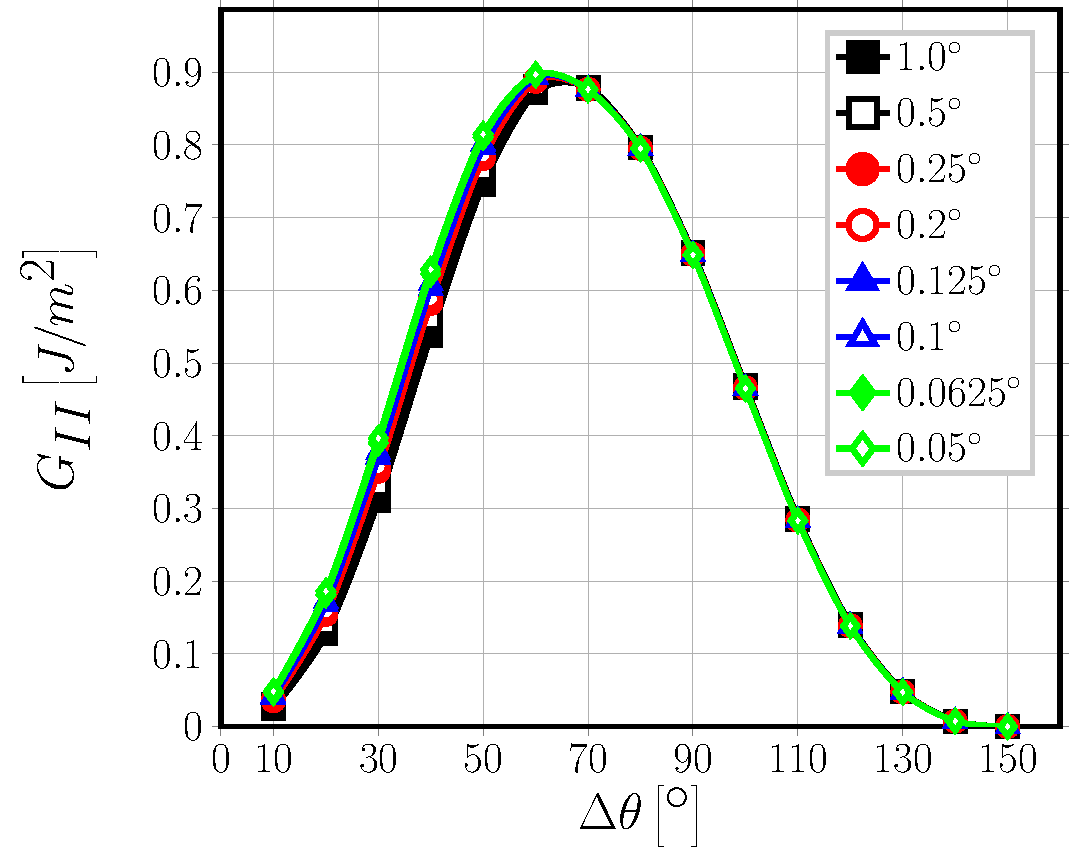
\includegraphics[width=0.6\textwidth]{Vf0_1-free-2nd-GII.pdf}
\end{figure}
$\rightarrow 1\times1-free, V_{f}=0.1\%, 2^{nd}\ order\ elements$ 
\end{frame}

\addtocounter{framenumber}{-1}

\begin{frame}
\frametitle{\vspace{0.25cm}\small $G_{II}$}
\vspace{-.75cm}
\centering
\begin{figure}
\centering
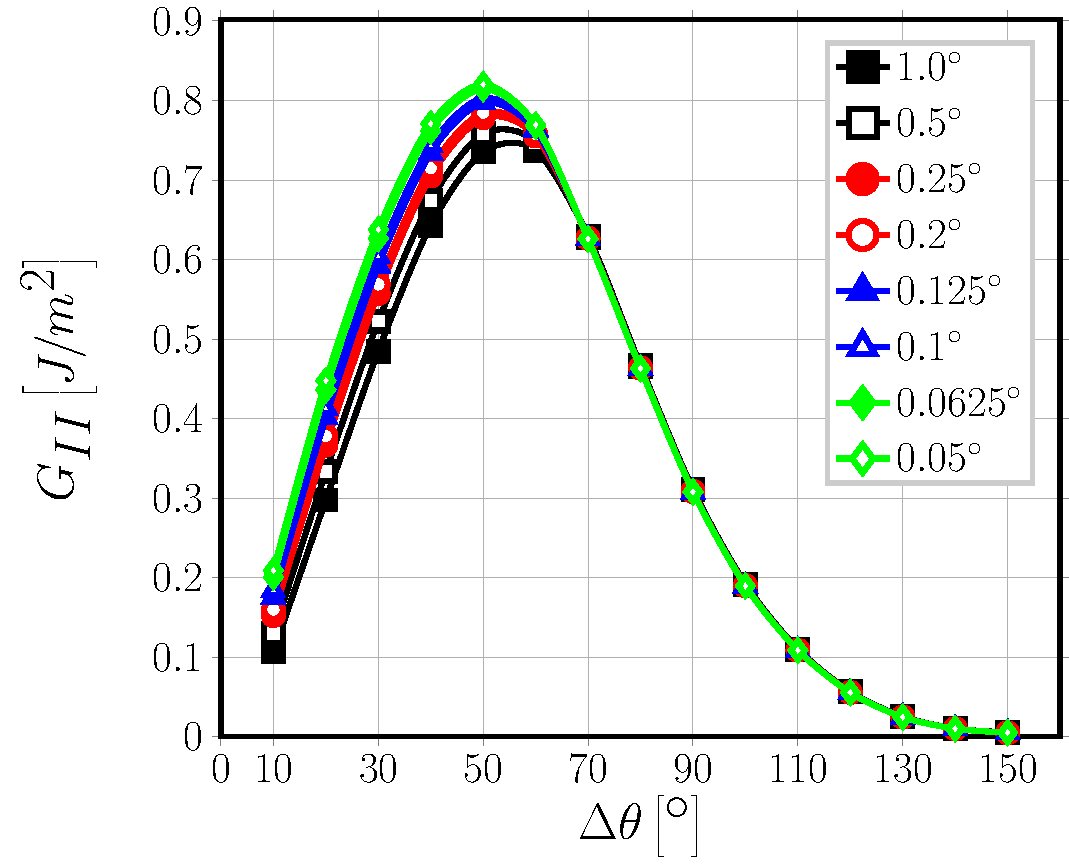
\includegraphics[width=0.6\textwidth]{Vf40-free-1st-GII.pdf}
\end{figure}
$\rightarrow 1\times1-free, V_{f}=40\%, 1^{st}\ order\ elements$ 
\end{frame}

\addtocounter{framenumber}{-1}

\begin{frame}
\frametitle{\vspace{0.25cm}\small $G_{II}$}
\vspace{-.75cm}
\centering
\begin{figure}
\centering
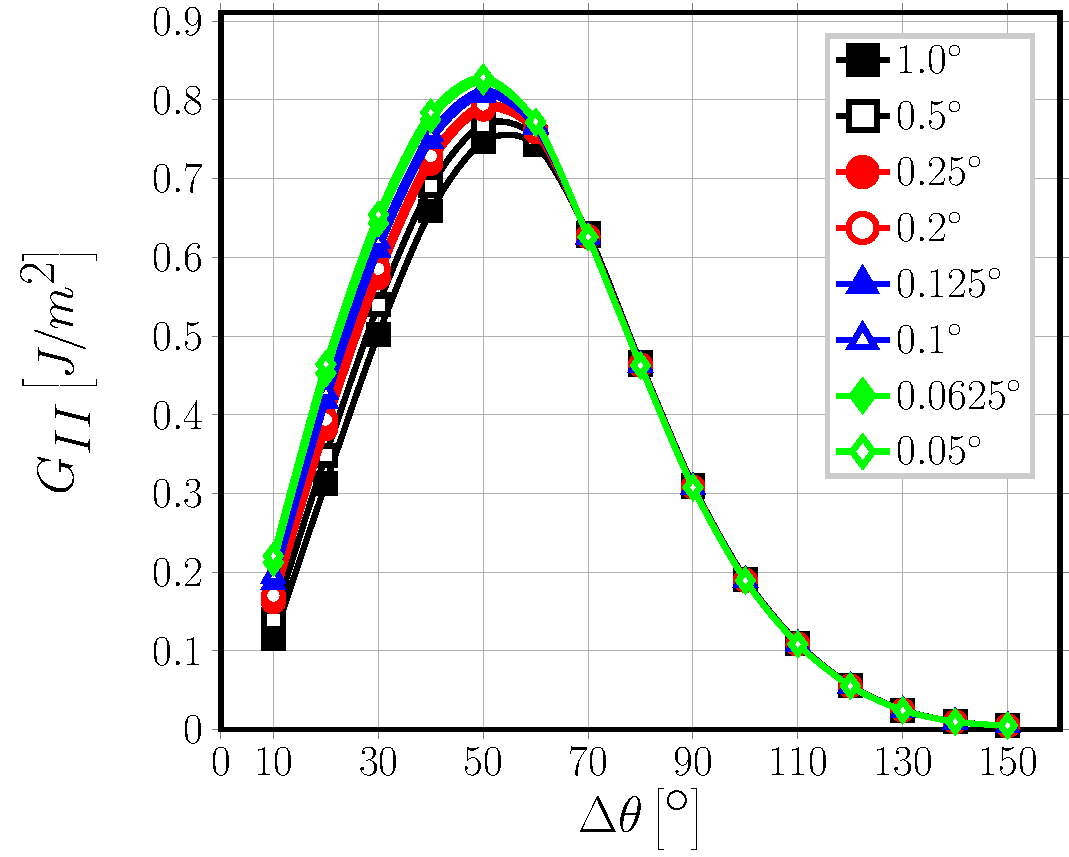
\includegraphics[width=0.6\textwidth]{Vf40-free-2nd-GII.pdf}
\end{figure}
$\rightarrow 1\times1-free, V_{f}=40\%, 2^{nd}\ order\ elements$ 
\end{frame}

\subsection{Vectorial formulation of VCCT}

\begin{frame}
\frametitle{\vspace{0.25cm}\small Vectorial formulation of VCCT}
\vspace{-.75cm}
\centering
\begin{figure}
\centering
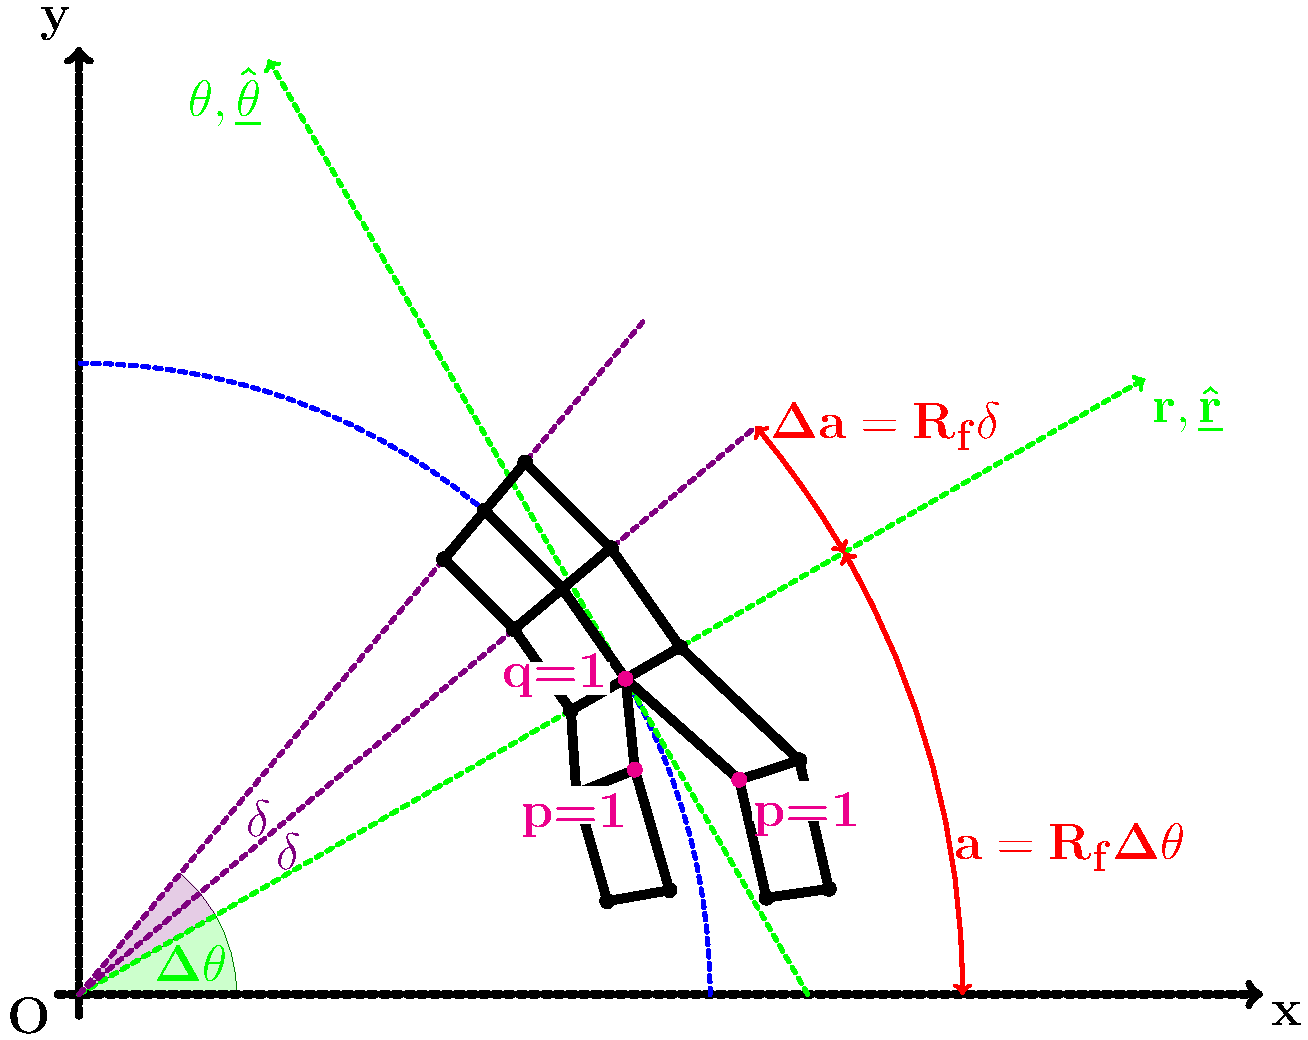
\includegraphics[height=0.5\textheight]{VCCT-linear.pdf}
\end{figure}
\begin{equation*}
\scriptsize
\begin{split}
G_{TOT} =&\frac{1}{2R_{f}\delta}\sum_{p=1}^{m+1}\sum_{q=1}^{m+1}Tr\left(\underline{\underline{Q}}_{\delta}\underline{\underline{R}}_{\Delta\theta}\underline{\underline{K}}_{xy,q}\underline{u}_{xy,q}\underline{u}_{xy,p}^{T}\underline{\underline{R}}_{\Delta\theta}^{T}\underline{\underline{P}}_{\delta}^{T}\underline{\underline{T}}_{pq}^{T}\right)+\\&+\frac{1}{2R_{f}\delta}\sum_{p=1}^{m+1}\sum_{q=1}^{m+1}Tr\left(\underline{\underline{Q}}_{\delta}\underline{\underline{R}}_{\Delta\theta}\underline{\widetilde{F}}_{xy,q}\underline{u}_{xy,p}^{T}\underline{\underline{R}}_{\Delta\theta}^{T}\underline{\underline{P}}_{\delta}^{T}\underline{\underline{T}}_{pq}^{T}\right)
\end{split}
\end{equation*}
\end{frame}

\addtocounter{framenumber}{-1}

\begin{frame}
\frametitle{\vspace{0.25cm}\small Vectorial formulation of VCCT}
\vspace{-.75cm}
\centering
\begin{figure}
\centering
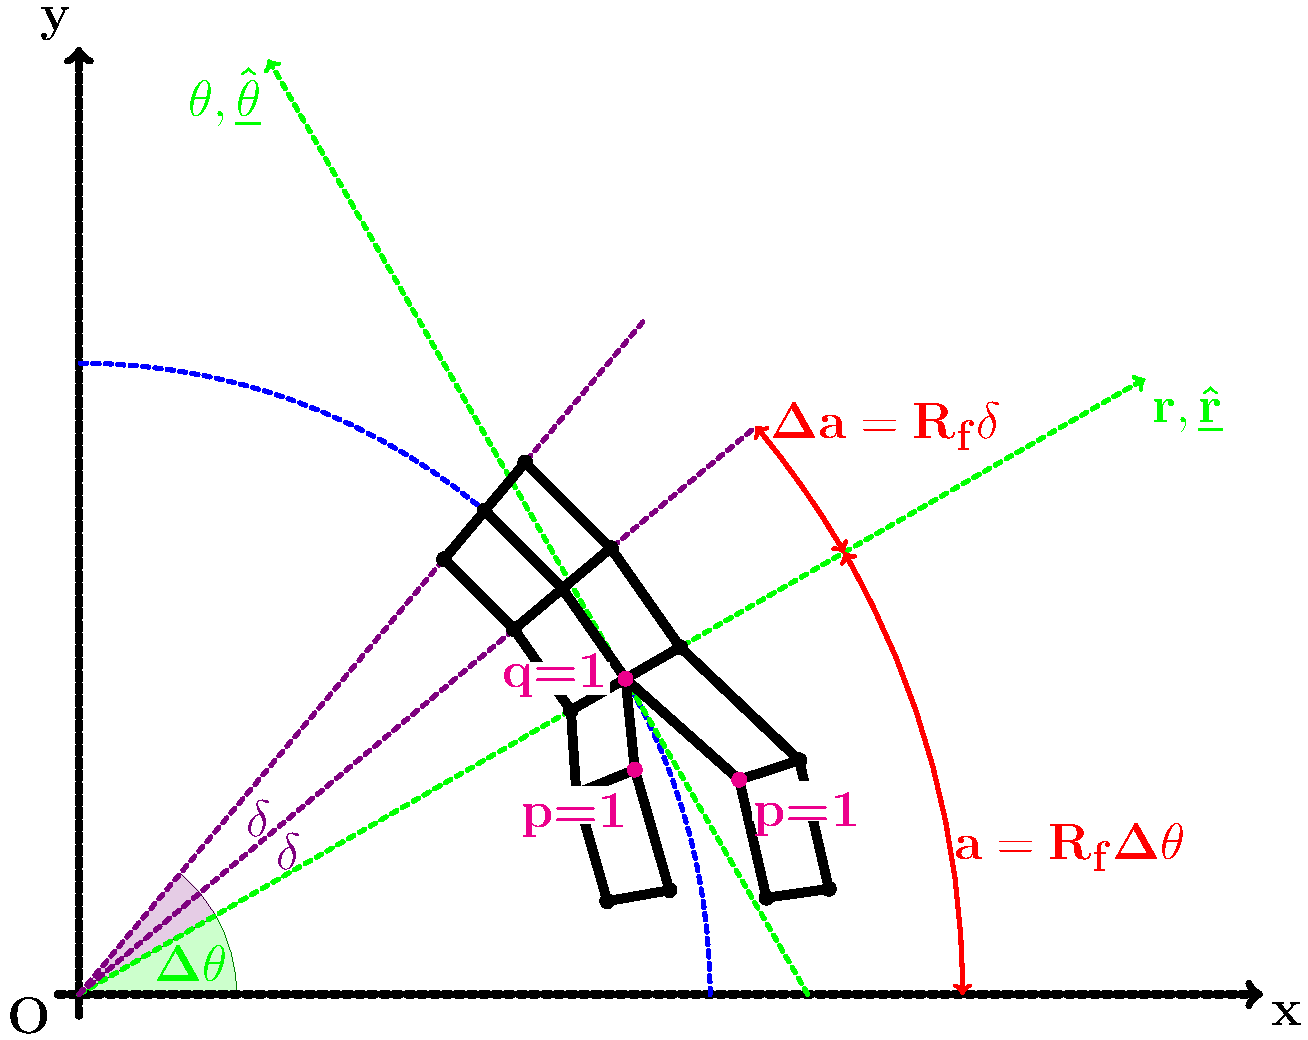
\includegraphics[height=0.5\textheight]{VCCT-linear.pdf}
\end{figure}
\begin{equation*}
\scriptsize
\begin{split}
\underline{G}=\begin{bmatrix}
G_{I} \\
G_{II}
\end{bmatrix}=&\frac{1}{2R_{f}\delta}\sum_{p=1}^{m+1}\sum_{q=1}^{m+1}Diag\left(\underline{\underline{Q}}_{\delta}\underline{\underline{R}}_{\Delta\theta}\underline{\underline{K}}_{xy,q}\underline{u}_{xy,q}\underline{u}_{xy,p}^{T}\underline{\underline{R}}_{\Delta\theta}^{T}\underline{\underline{P}}_{\delta}^{T}\underline{\underline{T}}_{pq}^{T}\right)+\\
&+\frac{1}{2R_{f}\delta}\sum_{p=1}^{m+1}\sum_{q=1}^{m+1}Diag\left(\underline{\underline{Q}}_{\delta}\underline{\underline{R}}_{\Delta\theta}\underline{\underline{\widetilde{K}}}_{N,q}\underline{u}_{N}\underline{u}_{xy,p}^{T}\underline{\underline{R}}_{\Delta\theta}^{T}\underline{\underline{P}}_{\delta}^{T}\underline{\underline{T}}_{pq}^{T}\right)
\end{split}
\end{equation*}
\end{frame}

\subsection{Asymptotic behavior}

\begin{frame}
\frametitle{\vspace{0.25cm}\small Asymptotic behavior}
\vspace{-1.25cm}
\centering
\begin{equation*}
\scriptsize
\frac{\partial \underline{G}}{\partial \delta}=\frac{1}{\delta}\underline{G}+\frac{1}{2R_{f}\delta}\left(\dots\right)
\end{equation*}
\begin{equation*}
\scriptsize
u\left(\delta\right)\sim \sqrt{\delta}\left(\sin,\cos\right)\left(\epsilon\log{\delta}\right)\quad\text{with}\quad\epsilon=\frac{1}{2\pi}\log{\left(\frac{1-\beta}{1+\beta}\right)}
\end{equation*}
\begin{equation*}
\scriptsize
\lim_{\delta\rightarrow 0}\frac{\partial \underline{G}}{\partial \delta}\sim\frac{1}{\delta}\quad\xrightarrow{\int d\delta}\quad\lim_{\delta\rightarrow 0}\underline{G}\sim \underline{A}\log(\delta)+\underline{B}.
\end{equation*}
\end{frame}

\subsection{Numerical convergence}

\begin{frame}
\frametitle{\vspace{0.25cm}\small Numerical convergence: $G_{I}$}
\vspace{-.75cm}
\centering
\begin{figure}
\centering
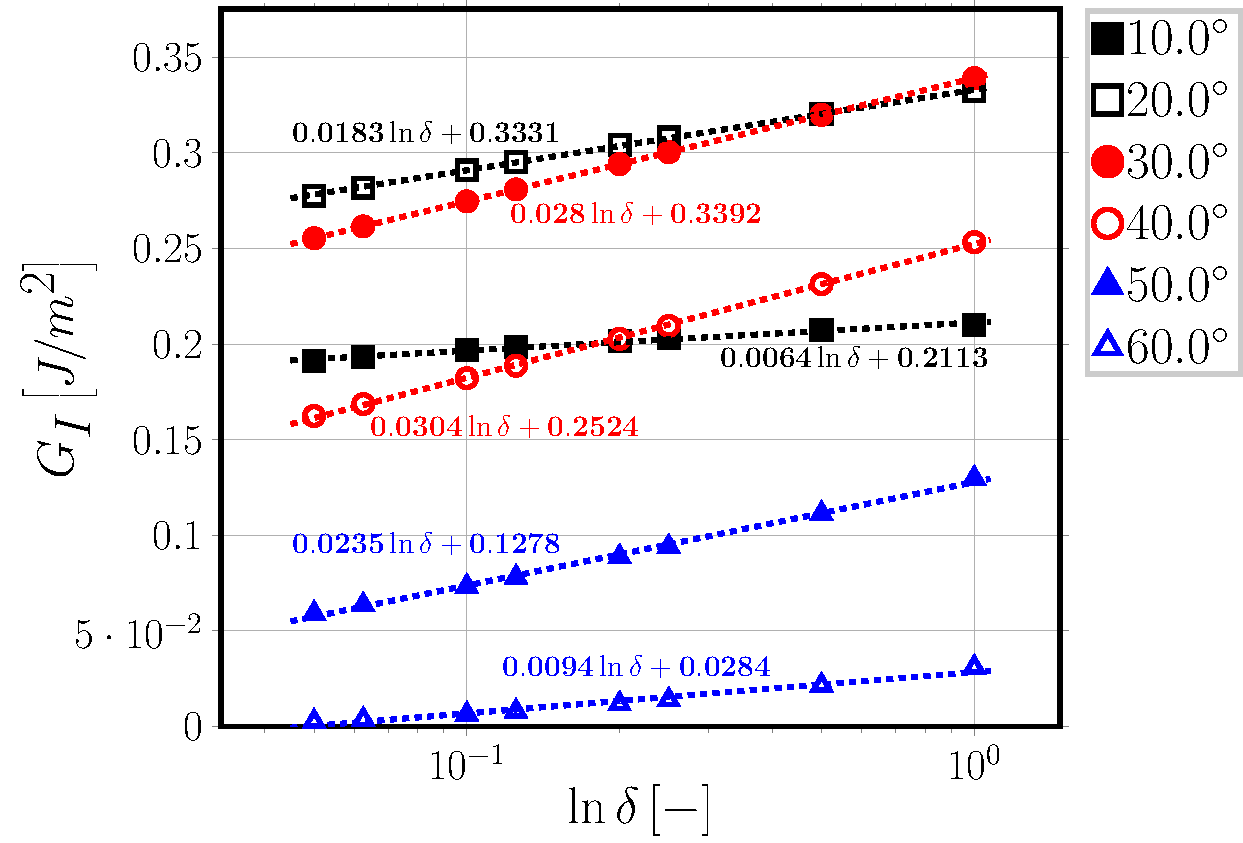
\includegraphics[width=0.6\textwidth]{Vf0_1-free-1st-semilogvsDelta-GI.pdf}
\end{figure}
$\rightarrow 1\times1-free, V_{f}=0.1\%, 1^{st}\ order\ elements$ 
\end{frame}

\addtocounter{framenumber}{-1}

\begin{frame}
\frametitle{\vspace{0.25cm}\small Numerical convergence: $G_{I}$}
\vspace{-.75cm}
\centering
\begin{figure}
\centering
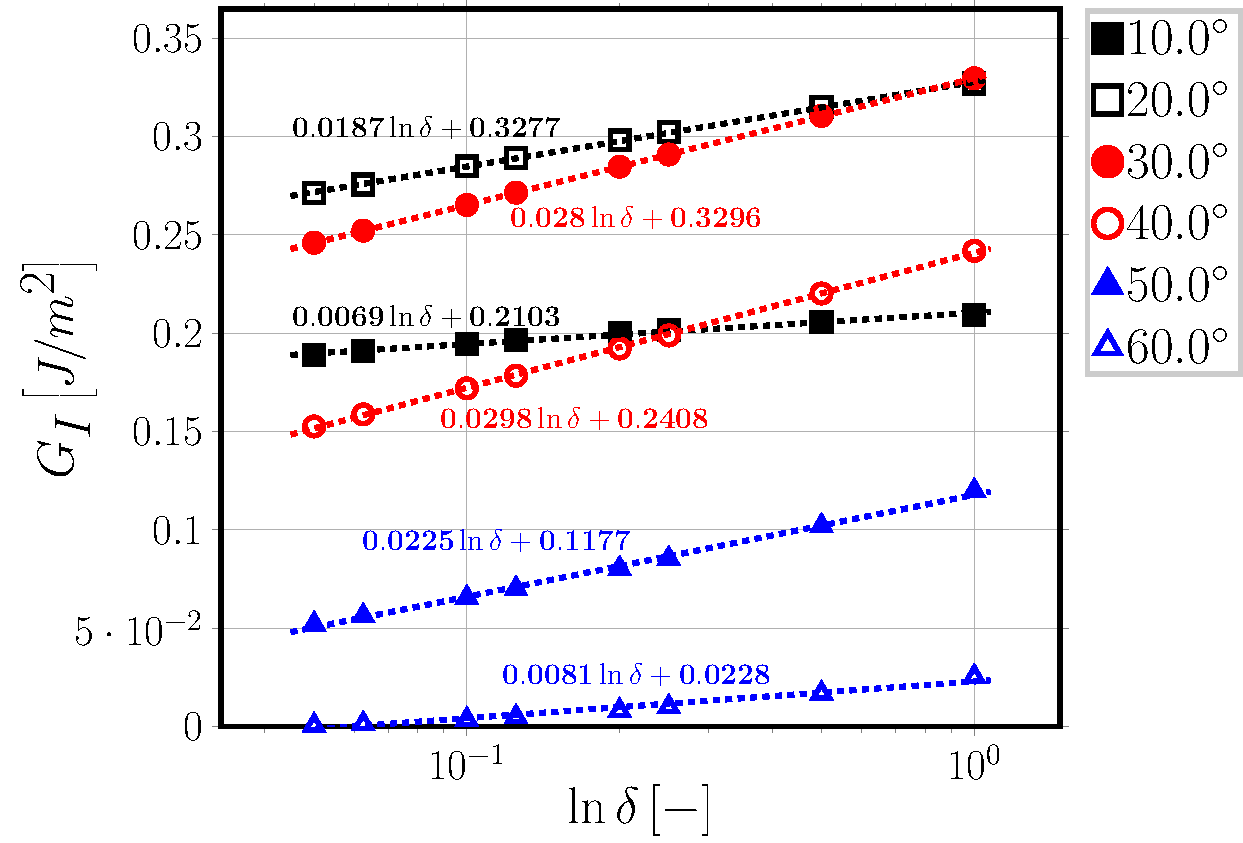
\includegraphics[width=0.6\textwidth]{Vf0_1-free-2nd-semilogvsDelta-GI.pdf}
\end{figure}
$\rightarrow 1\times1-free, V_{f}=0.1\%, 2^{nd}\ order\ elements$ 
\end{frame}

\addtocounter{framenumber}{-1}

\begin{frame}
\frametitle{\vspace{0.25cm}\small Numerical convergence: $G_{I}$}
\vspace{-.75cm}
\centering
\begin{figure}
\centering
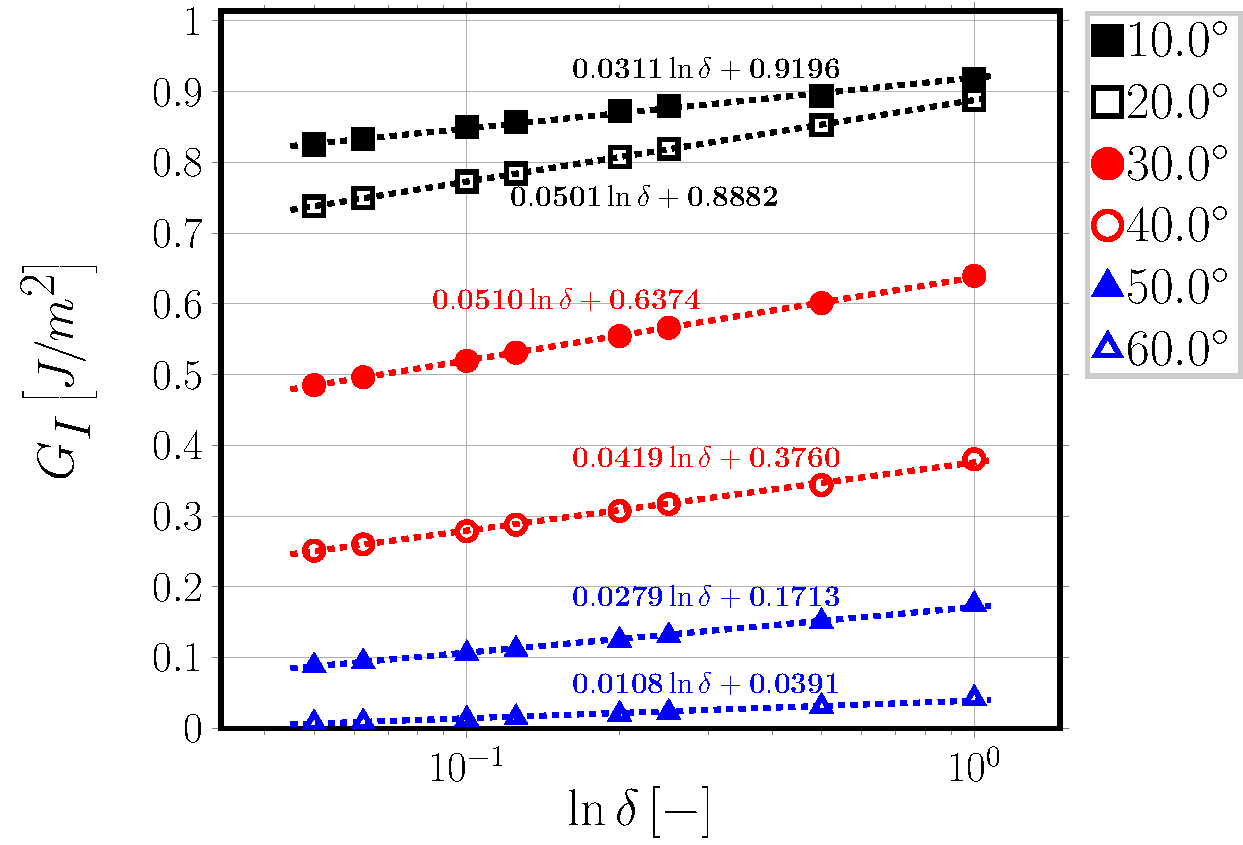
\includegraphics[width=0.6\textwidth]{Vf40-free-1st-semilogvsDelta-GI.pdf}
\end{figure}
$\rightarrow 1\times1-free, V_{f}=40\%, 1^{st}\ order\ elements$ 
\end{frame}

\addtocounter{framenumber}{-1}

\begin{frame}
\frametitle{\vspace{0.25cm}\small Numerical convergence: $G_{I}$}
\vspace{-.75cm}
\centering
\begin{figure}
\centering
\includegraphics[width=0.6\textwidth]{Vf40-free-2nd-semilogvsDelta-GI.pdf}
\end{figure}
$\rightarrow 1\times1-free, V_{f}=40\%, 2^{nd}\ order\ elements$ 
\end{frame}

\begin{frame}
\frametitle{\vspace{0.25cm}\small Numerical convergence: $G_{II}$}
\vspace{-.75cm}
\centering
\begin{figure}
\centering
\includegraphics[width=0.6\textwidth]{Vf0_1-free-1st-semilogvsDelta-GII.pdf}
\end{figure}
$\rightarrow 1\times1-free, V_{f}=0.1\%, 1^{st}\ order\ elements$ 
\end{frame}

\addtocounter{framenumber}{-1}

\begin{frame}
\frametitle{\vspace{0.25cm}\small Numerical convergence: $G_{II}$}
\vspace{-.75cm}
\centering
\begin{figure}
\centering
\includegraphics[width=0.6\textwidth]{Vf0_1-free-2nd-semilogvsDelta-GII.pdf}
\end{figure}
$\rightarrow 1\times1-free, V_{f}=0.1\%, 2^{nd}\ order\ elements$ 
\end{frame}

\addtocounter{framenumber}{-1}

\begin{frame}
\frametitle{\vspace{0.25cm}\small Numerical convergence: $G_{II}$}
\vspace{-.75cm}
\centering
\begin{figure}
\centering
\includegraphics[width=0.6\textwidth]{Vf40-free-1st-semilogvsDelta-GII.pdf}
\end{figure}
$\rightarrow 1\times1-free, V_{f}=40\%, 1^{st}\ order\ elements$ 
\end{frame}

\addtocounter{framenumber}{-1}

\begin{frame}
\frametitle{\vspace{0.25cm}\small Numerical convergence: $G_{II}$}
\vspace{-.75cm}
\centering
\begin{figure}
\centering
\includegraphics[width=0.6\textwidth]{Vf40-free-2nd-semilogvsDelta-GII.pdf}
\end{figure}
$\rightarrow 1\times1-free, V_{f}=40\%, 2^{nd}\ order\ elements$ 
\end{frame}

\subsection{$\delta$ selection}

\begin{frame}
\frametitle{\vspace{0.25cm}\small $\delta$ selection}
\vspace{-.75cm}
\centering
\begin{figure}
\centering
\includegraphics[width=0.6\textwidth]{validation-VCCT.pdf}
\end{figure}
\vspace{-.5cm}
\centering
\pgfmathsetmacro\fontsizeref{4.5}
\pgfmathsetmacro\stretchref{1}
{\centering\fontsize{\fontsizeref}{\stretchref} \selectfont \href{https://doi.org/10.1115/1.2711220
}{Par\'is et al., J. Appl. Mech.\textbf{74} (4), 2007.}}\\\vspace{-5pt}
{\centering\fontsize{\fontsizeref}{\stretchref} \selectfont \href{https://doi.org/10.1016/j.engfracmech.2016.01.022
}{Sandino et al., Eng. Fract. Mech.\textbf{168}, 2016.}}\\\vspace{.1cm}
$\rightarrow 1\times1-free, V_{f}=0.01\%, 2^{nd}\ order\ elements,\delta=0.05^{\circ}$ 
\end{frame}

\section{Debond Initiation}

\subsection{$\mathbf{\sigma_{rr}}$ vs $\mathbf{\tau_{r\theta}}$}

\begin{frame}
\frametitle{\vspace{0.2cm}\small $\mathbf{\sigma_{rr}}$ vs $\mathbf{\tau_{r\theta}}$: radial stress vs tangential shear at the interface}
\vspace{-.75cm}
\centering
\begin{columns}[c]
\centering
\begin{column}{0.5\textwidth}
\centering
\begin{figure}
\centering
\includegraphics[width=\columnwidth]{vf60-nodamage-sigmar-notol.pdf}
\end{figure}
\end{column}
\begin{column}{0.5\textwidth}
\centering
\begin{figure}
\centering
\includegraphics[width=\columnwidth]{vf60-nodamage-taurt.pdf}
\end{figure}
\end{column}
\end{columns}
\vspace{-0.4cm}
\centering
\begin{figure}
\centering
\includegraphics[width=\textwidth]{refAngle.pdf}
\end{figure}
\end{frame}

\addtocounter{framenumber}{-1}

\begin{frame}
\frametitle{\vspace{0.2cm}\small $\mathbf{\sigma_{rr}}$ vs $\mathbf{\tau_{r\theta}}$: radial stress vs tangential shear at the interface}
\vspace{-.75cm}
\centering
\begin{columns}[c]
\centering
\begin{column}{0.5\textwidth}
\centering
\begin{figure}
\centering
\includegraphics[width=\columnwidth]{vf60-nodamage-sigmar.pdf}
\end{figure}
\end{column}
\begin{column}{0.5\textwidth}
\centering
\begin{figure}
\centering
\includegraphics[width=\columnwidth]{vf60-nodamage-taurt.pdf}
\end{figure}
\end{column}
\end{columns}
\vspace{-0.4cm}
\centering
\begin{figure}
\centering
\includegraphics[width=\textwidth]{refAngle.pdf}
\end{figure}
\end{frame}

\subsection{$\sigma_{LHS}$}

\begin{frame}
\frametitle{\vspace{0.2cm}\small $\mathbf{\sigma_{LHS}}$: local hydrostatic stress at the interface}
\vspace{-.75cm}
\centering
\begin{columns}[c]
\centering
\begin{column}{0.5\textwidth}
\centering
\begin{figure}
\centering
\includegraphics[width=\columnwidth]{vf60-nodamage-p2D-notol.pdf}
\end{figure}
\vspace{-0.5cm}
\scriptsize
\begin{equation*}
\sigma^{2D}_{LHS}=\frac{\sigma_{rr}+\sigma_{\theta\theta}}{2}
\end{equation*}
\end{column}
\begin{column}{0.5\textwidth}
\centering
\begin{figure}
\centering
\includegraphics[width=\columnwidth]{vf60-nodamage-p3D-notol.pdf}
\end{figure}
\vspace{-0.5cm}
\scriptsize
\begin{equation*}
\sigma^{3D}_{LHS}=\frac{\sigma_{rr}+\sigma_{\theta\theta}+\sigma_{yy}}{3}
\end{equation*}
\end{column}
\end{columns}
\vspace{-0.45cm}
\centering
\begin{figure}
\centering
\includegraphics[width=\textwidth]{refAngle.pdf}
\end{figure}
\end{frame}

\addtocounter{framenumber}{-1}

\begin{frame}
\frametitle{\vspace{0.2cm}\small $\mathbf{\sigma_{LHS}}$: local hydrostatic stress at the interface}
\vspace{-.75cm}
\centering
\begin{columns}[c]
\centering
\begin{column}{0.5\textwidth}
\centering
\begin{figure}
\centering
\includegraphics[width=\columnwidth]{vf60-nodamage-p2D.pdf}
\end{figure}
\vspace{-0.5cm}
\scriptsize
\begin{equation*}
\sigma^{2D}_{LHS}=\frac{\sigma_{rr}+\sigma_{\theta\theta}}{2}
\end{equation*}
\end{column}
\begin{column}{0.5\textwidth}
\centering
\begin{figure}
\centering
\includegraphics[width=\columnwidth]{vf60-nodamage-p3D.pdf}
\end{figure}
\vspace{-0.5cm}
\scriptsize
\begin{equation*}
\sigma^{3D}_{LHS}=\frac{\sigma_{rr}+\sigma_{\theta\theta}+\sigma_{yy}}{3}
\end{equation*}
\end{column}
\end{columns}
\vspace{-0.45cm}
\centering
\begin{figure}
\centering
\includegraphics[width=\textwidth]{refAngle.pdf}
\end{figure}
\end{frame}

\subsection{$\sigma_{vM}$}

\begin{frame}
\frametitle{\vspace{0.2cm}\small $\mathbf{\sigma_{vM}}$: von Mises stress at the interface}
\vspace{-.75cm}
\centering
\begin{columns}[c]
\centering
\begin{column}{0.5\textwidth}
\centering
\begin{figure}
\centering
\includegraphics[width=\columnwidth]{vf60-nodamage-vM2D-notol.pdf}
\end{figure}
\vspace{-0.9cm}
\scriptsize
\begin{equation*}
\sigma^{2D}_{vM}=\sqrt{\left(\sigma_{rr}-\sigma_{\theta\theta}\right)^{2}+3\tau_{12}^{2}}
\end{equation*}
\end{column}
\begin{column}{0.5\textwidth}
\centering
\begin{figure}
\centering
\includegraphics[width=\columnwidth]{vf60-nodamage-vM3D.pdf}
\end{figure}
\vspace{-0.3cm}
\scriptsize
\begin{equation*}
\sigma^{3D}_{LHS}=\frac{3}{2}s_{ij}s_{ij}\quad s_{ij}=\sigma_{ij}-\frac{1}{3}\sigma_{kk}\delta_{ij}
\end{equation*}
\end{column}
\end{columns}
\vspace{-0.3cm}
\centering
\begin{figure}
\centering
\includegraphics[width=\textwidth]{refAngle.pdf}
\end{figure}
\end{frame}

\addtocounter{framenumber}{-1}

\begin{frame}
\frametitle{\vspace{0.2cm}\small $\mathbf{\sigma_{vM}}$: von Mises stress at the interface}
\vspace{-.75cm}
\centering
\begin{columns}[c]
\centering
\begin{column}{0.5\textwidth}
\centering
\begin{figure}
\centering
\includegraphics[width=\columnwidth]{vf60-nodamage-vM2D.pdf}
\end{figure}
\vspace{-0.9cm}
\scriptsize
\begin{equation*}
\qquad\qquad\sigma^{2D}_{vM}=\sqrt{\left(\sigma_{rr}-\sigma_{\theta\theta}\right)^{2}+3\tau_{12}^{2}}
\end{equation*}
\end{column}
\begin{column}{0.5\textwidth}
\centering
\begin{figure}
\centering
\includegraphics[width=\columnwidth]{vf60-nodamage-vM3D.pdf}
\end{figure}
\vspace{-0.3cm}
\scriptsize
\begin{equation*}
\sigma^{3D}_{LHS}=\frac{3}{2}s_{ij}s_{ij}\quad s_{ij}=\sigma_{ij}-\frac{1}{3}\sigma_{kk}\delta_{ij}
\end{equation*}
\end{column}
\end{columns}
\vspace{-0.3cm}
\centering
\begin{figure}
\centering
\includegraphics[width=\textwidth]{refAngle.pdf}
\end{figure}
\end{frame}

\subsection{$\sigma_{I}$}

\begin{frame}
\frametitle{\vspace{0.2cm}\small $\mathbf{\sigma_{I}}$: maximum principal stress at the interface}
\vspace{-.75cm}
\centering
\begin{columns}[c]
\centering
\begin{column}{0.5\textwidth}
\centering
\begin{figure}
\centering
\includegraphics[width=\columnwidth]{vf60-nodamage-sigmaI2D-notol.pdf}
\end{figure}
\end{column}
\begin{column}{0.5\textwidth}
\centering
\begin{figure}
\centering
\includegraphics[width=\columnwidth]{vf60-nodamage-sigmaI3D-notol.pdf}
\end{figure}
\end{column}
\end{columns}
\vspace{-0.4cm}
\centering
\begin{figure}
\centering
\includegraphics[width=\textwidth]{refAngle.pdf}
\end{figure}
\end{frame}

\addtocounter{framenumber}{-1}

\begin{frame}
\frametitle{\vspace{0.2cm}\small $\mathbf{\sigma_{I}}$: maximum principal stress at the interface}
\vspace{-.75cm}
\centering
\begin{columns}[c]
\centering
\begin{column}{0.5\textwidth}
\centering
\begin{figure}
\centering
\includegraphics[width=\columnwidth]{vf60-nodamage-sigmaI2D.pdf}
\end{figure}
\end{column}
\begin{column}{0.5\textwidth}
\centering
\begin{figure}
\centering
\includegraphics[width=\columnwidth]{vf60-nodamage-sigmaI3D.pdf}
\end{figure}
\end{column}
\end{columns}
\vspace{-0.4cm}
\centering
\begin{figure}
\centering
\includegraphics[width=\textwidth]{refAngle.pdf}
\end{figure}
\end{frame}

\subsection{Observations}

\begin{frame}
\frametitle{Observations}
\vspace{-0.5cm}
\centering
\scriptsize
\begin{itemize}[label=\ding{212}]
\item For all stresses analyzed, no significant difference is present between the different RUCs for $\psi\leq10^{\circ}$;
\item for all stresses analyzed, no difference can be observed by increasing $k$ when $k\geq3$;
\item for all stresses analyzed, no difference can be observed between $1\times  k-free$ and $1\times  k-1\cdot t_{90^{\circ}}$ for $k\geq3$;
\item $\sigma_{rr}$, $\sigma_{LHS,2D}$, $\sigma_{LHS,3D}$, $\sigma_{vM,2D}$, $\sigma_{LMPS,2D}$ and $\sigma_{LMPS,3D}$ all reach their peak value at $0^{\circ}$ and $180^{\circ}$ and decrease to $99\%$ the peak value between $2^{\circ}$ and $8^{\circ}$, to $95\%$ the peak value between $6^{\circ}$ and $12^{\circ}$ and to $90\%$ the peak value between $8^{\circ}$ and $15^{\circ}$ from the occurrence of the maximum.
\end{itemize}
\begin{alertblock}{\centering\scriptsize\bf It seems reasonable to conclude that...}
...a stress-based criterion would predict, irrespectively of the specific criterion chosen, the onset of an interface crack at $0^{\circ}$ or $180^{\circ}$ with an initial size at least comprised in the range $2^{\circ}-8^{\circ}$ ($1\%$ margin) and likely in the range $6^{\circ}-12^{\circ}$ ($5\%$ margin). Thus, no evident effect of $90^{\circ}$ or $0^{\circ}$ layer thickness can be observed.
\end{alertblock}
\end{frame}

\section{Debond Propagation}

\subsection{Debond Interaction: Horizontal}

\begin{frame}
\frametitle{\vspace{0.2cm}\small Interaction of Debonds: Crack Shielding}
\vspace{-.75cm}
\centering
\begin{columns}[c]
\centering
\begin{column}{0.5\textwidth}
\centering
\begin{figure}
\centering
\includegraphics[width=\columnwidth]{nxk-1-vf60-GI-crackshield21.pdf}
\end{figure}
\end{column}
\begin{column}{0.5\textwidth}
\centering
\begin{figure}
\centering
\includegraphics[width=\columnwidth]{nxk-1-vf60-GII-crackshield21.pdf}
\end{figure}
\end{column}
\end{columns}
\begin{figure}
\centering
\includegraphics[width=\textwidth]{twofibers-sameside-crackshielding21.pdf}
\end{figure}
\end{frame}

\addtocounter{framenumber}{-1}

\begin{frame}
\frametitle{\vspace{0.2cm}\small Interaction of Debonds: Crack Shielding}
\vspace{-.75cm}
\centering
\begin{columns}[c]
\centering
\begin{column}{0.5\textwidth}
\centering
\begin{figure}
\centering
\includegraphics[width=\columnwidth]{nxk-1-vf60-GI-crackshield3.pdf}
\end{figure}
\end{column}
\begin{column}{0.5\textwidth}
\centering
\begin{figure}
\centering
\includegraphics[width=\columnwidth]{nxk-1-vf60-GII-crackshield3.pdf}
\end{figure}
\end{column}
\end{columns}
\begin{figure}
\centering
\includegraphics[width=\textwidth]{twofibers-sameside-crackshielding3.pdf}
\end{figure}
\end{frame}

\addtocounter{framenumber}{-1}

\begin{frame}
\frametitle{\vspace{0.2cm}\small Interaction of Debonds: Crack Shielding}
\vspace{-.75cm}
\centering
\begin{columns}[c]
\centering
\begin{column}{0.5\textwidth}
\centering
\begin{figure}
\centering
\includegraphics[width=\columnwidth]{nxk-1-vf60-GI-crackshield1.pdf}
\end{figure}
\end{column}
\begin{column}{0.5\textwidth}
\centering
\begin{figure}
\centering
\includegraphics[width=\columnwidth]{nxk-1-vf60-GII-crackshield1.pdf}
\end{figure}
\end{column}
\end{columns}
\begin{figure}
\centering
\includegraphics[width=\textwidth]{twofibers-sameside-crackshielding1.pdf}
\end{figure}
\end{frame}

\begin{frame}
\frametitle{\vspace{0.2cm}\small Interaction of Debonds: Strain Magnification}
\vspace{-.75cm}
\centering
\begin{columns}[c]
\centering
\begin{column}{0.5\textwidth}
\centering
\begin{figure}
\centering
\includegraphics[width=\columnwidth]{nxk-1-vf60-GI-strainmagni1.pdf}
\end{figure}
\end{column}
\begin{column}{0.5\textwidth}
\centering
\begin{figure}
\centering
\includegraphics[width=\columnwidth]{nxk-1-vf60-GII-strainmagni1.pdf}
\end{figure}
\end{column}
\end{columns}
\vspace{-0.25cm}
\centering
\begin{figure}
\centering
\includegraphics[width=0.275\textwidth]{twofibers-sameside-strainmagni1.pdf}
\end{figure}
\end{frame}

\addtocounter{framenumber}{-1}

\begin{frame}
\frametitle{\vspace{0.2cm}\small Interaction of Debonds: Strain Magnification}
\vspace{-.75cm}
\centering
\begin{columns}[c]
\centering
\begin{column}{0.5\textwidth}
\centering
\begin{figure}
\centering
\includegraphics[width=\columnwidth]{nxk-1-vf60-GI-strainmagni3.pdf}
\end{figure}
\end{column}
\begin{column}{0.5\textwidth}
\centering
\begin{figure}
\centering
\includegraphics[width=\columnwidth]{nxk-1-vf60-GII-strainmagni3.pdf}
\end{figure}
\end{column}
\end{columns}
\vspace{-0.25cm}
\begin{figure}
\centering
\includegraphics[width=0.325\textwidth]{twofibers-sameside-strainmagni3.pdf}
\end{figure}
\end{frame}

\addtocounter{framenumber}{-1}

\begin{frame}
\frametitle{\vspace{0.2cm}\small Interaction of Debonds: Strain Magnification}
\vspace{-.75cm}
\centering
\begin{columns}[c]
\centering
\begin{column}{0.5\textwidth}
\centering
\begin{figure}
\centering
\includegraphics[width=\columnwidth]{nxk-1-vf60-GI-strainmagni21.pdf}
\end{figure}
\end{column}
\begin{column}{0.5\textwidth}
\centering
\begin{figure}
\centering
\includegraphics[width=\columnwidth]{nxk-1-vf60-GII-strainmagni21.pdf}
\end{figure}
\end{column}
\end{columns}
\vspace{-0.25cm}
\begin{figure}
\centering
\includegraphics[width=\textwidth]{twofibers-sameside-strainmagni21.pdf}
\end{figure}
\end{frame}

\subsection{Debond Interaction: Vertical}

\begin{frame}
\frametitle{\vspace{0.2cm}\small Consecutive Debonds: Mode I}
\vspace{-0.5cm}
\centering
\begin{columns}
\centering
\begin{column}{0.65\textwidth}
\centering
\begin{figure}
\centering
\includegraphics[width=\columnwidth]{nx1-coupling-vf60-GI.pdf}
\end{figure}
\end{column}
\begin{column}{0.35\textwidth}
\centering
\begin{figure}
\centering
\includegraphics[width=\columnwidth]{twofibers-sameside-dtheta100.pdf}
\end{figure}
\vspace{-0.5cm}
\begin{figure}
\centering
\includegraphics[width=\columnwidth]{twofibers-oppositeside-dtheta80.pdf}
\end{figure}
\end{column}
\end{columns}
\end{frame}

\begin{frame}
\frametitle{\vspace{0.2cm}\small Consecutive Debonds: Mode II}
\vspace{-0.5cm}
\centering
\begin{columns}
\centering
\begin{column}{0.65\textwidth}
\centering
\begin{figure}
\centering
\includegraphics[width=\columnwidth]{nx1-coupling-vf60-GII-dtheta80.pdf}
\end{figure}
\end{column}
\begin{column}{0.35\textwidth}
\centering
\begin{figure}
\centering
\includegraphics[width=\columnwidth]{twofibers-sameside-dtheta80.pdf}
\end{figure}
\vspace{-0.5cm}
\begin{figure}
\centering
\includegraphics[width=\columnwidth]{twofibers-oppositeside-dtheta80.pdf}
\end{figure}
\end{column}
\end{columns}
\end{frame}

\addtocounter{framenumber}{-1}

\begin{frame}
\frametitle{\vspace{0.2cm}\small Consecutive Debonds: Mode II}
\vspace{-0.5cm}
\centering
\begin{columns}
\centering
\begin{column}{0.65\textwidth}
\centering
\begin{figure}
\centering
\includegraphics[width=\columnwidth]{nx1-coupling-vf60-GII-dtheta110.pdf}
\end{figure}
\end{column}
\begin{column}{0.35\textwidth}
\centering
\begin{figure}
\centering
\includegraphics[width=\columnwidth]{twofibers-sameside-dtheta110.pdf}
\end{figure}
\vspace{-0.5cm}
\begin{figure}
\centering
\includegraphics[width=\columnwidth]{twofibers-oppositeside-dtheta110.pdf}
\end{figure}
\end{column}
\end{columns}
\end{frame}

\addtocounter{framenumber}{-1}

\begin{frame}
\frametitle{\vspace{0.2cm}\small Consecutive Debonds: Mode II}
\vspace{-0.5cm}
\centering
\begin{columns}
\centering
\begin{column}{0.65\textwidth}
\centering
\begin{figure}
\centering
\includegraphics[width=\columnwidth]{nx1-coupling-vf60-GII-dtheta150.pdf}
\end{figure}
\end{column}
\begin{column}{0.35\textwidth}
\centering
\begin{figure}
\centering
\includegraphics[width=\columnwidth]{twofibers-sameside-dtheta150.pdf}
\end{figure}
\vspace{-0.5cm}
\begin{figure}
\centering
\includegraphics[width=\columnwidth]{twofibers-oppositeside-dtheta150.pdf}
\end{figure}
\end{column}
\end{columns}
\end{frame}

\begin{frame}
\frametitle{\vspace{0.3cm}\small Non-Consecutive Debonds}
\vspace{-0.9cm}
\centering
\begin{columns}
\centering
\begin{column}{0.5\textwidth}
\centering
\begin{figure}
\centering
\includegraphics[width=\columnwidth]{nxk-coupling-vf60-GI.pdf}
\end{figure}
\vspace{-0.95cm}
\begin{figure}
\centering
\includegraphics[width=0.5\columnwidth]{twofibersbetweendebonds-sameside-dtheta80.pdf}
\end{figure}
\end{column}
\begin{column}{0.5\textwidth}
\centering
\begin{figure}
\centering
\includegraphics[width=\columnwidth]{nxk-coupling-vf60-GII.pdf}
\end{figure}
\vspace{-0.95cm}
\begin{figure}
\centering
\includegraphics[width=0.5\columnwidth]{twofibersbetweendebonds-oppositeside-dtheta80.pdf}
\end{figure}
\end{column}
\end{columns}
\end{frame}

\subsection{$0^{\circ}$ ply thickness}

\begin{frame}
\frametitle{\vspace{0.2cm}\small Effect of $0^{\circ}$ ply thickness}
\vspace{-.75cm}
\centering
\begin{columns}[c]
\centering
\begin{column}{0.5\textwidth}
\centering
\begin{figure}
\centering
\includegraphics[width=\columnwidth]{1x1-i-vf60-GI-zero.pdf}
\end{figure}
\end{column}
\begin{column}{0.5\textwidth}
\centering
\begin{figure}
\centering
\includegraphics[width=\columnwidth]{1x1-i-vf60-GII-zero.pdf}
\end{figure}
\end{column}
\end{columns}
\begin{figure}
\centering
\includegraphics[width=0.75\textwidth]{zeroplythickness.pdf}
\end{figure}
\end{frame}

\addtocounter{framenumber}{-1}

\begin{frame}
\frametitle{\vspace{0.2cm}\small Effect of $0^{\circ}$ ply thickness}
\vspace{-.75cm}
\centering
\begin{columns}[c]
\centering
\begin{column}{0.5\textwidth}
\centering
\begin{figure}
\centering
\includegraphics[width=\columnwidth]{1x1-i-vf60-GI-free.pdf}
\end{figure}
\end{column}
\begin{column}{0.5\textwidth}
\centering
\begin{figure}
\centering
\includegraphics[width=\columnwidth]{1x1-i-vf60-GII-free.pdf}
\end{figure}
\end{column}
\end{columns}
\begin{columns}[c]
\centering
\begin{column}{0.5\textwidth}
\begin{figure}
\centering
\includegraphics[width=\columnwidth]{zeroplythickness.pdf}
\end{figure}
\end{column}
\begin{column}{0.5\textwidth}
\centering
\begin{figure}
\centering
\includegraphics[width=\columnwidth]{zeroplythickness-eqBC.pdf}
\end{figure}
\end{column}
\end{columns}
\end{frame}

\addtocounter{framenumber}{-1}

\begin{frame}
\frametitle{\vspace{0.2cm}\small Effect of $0^{\circ}$ ply thickness}
\vspace{-.75cm}
\centering
\begin{columns}[c]
\centering
\begin{column}{0.5\textwidth}
\centering
\begin{figure}
\centering
\includegraphics[width=\columnwidth]{1x1-i-vf60-GI-coupling.pdf}
\end{figure}
\end{column}
\begin{column}{0.5\textwidth}
\centering
\begin{figure}
\centering
\includegraphics[width=\columnwidth]{1x1-i-vf60-GII-coupling.pdf}
\end{figure}
\end{column}
\end{columns}
\begin{columns}[c]
\centering
\begin{column}{0.5\textwidth}
\begin{figure}
\centering
\includegraphics[width=\columnwidth]{zeroplythickness.pdf}
\end{figure}
\end{column}
\begin{column}{0.5\textwidth}
\centering
\begin{figure}
\centering
\includegraphics[width=\columnwidth]{zeroplythickness-eqBC.pdf}
\end{figure}
\end{column}
\end{columns}
\end{frame}

\addtocounter{framenumber}{-1}

\begin{frame}
\frametitle{\vspace{0.2cm}\small Effect of $0^{\circ}$ ply thickness}
\vspace{-.75cm}
\centering
\begin{columns}[c]
\centering
\begin{column}{0.5\textwidth}
\centering
\begin{figure}
\centering
\includegraphics[width=\columnwidth]{1x1-i-vf60-GI.pdf}
\end{figure}
\end{column}
\begin{column}{0.5\textwidth}
\centering
\begin{figure}
\centering
\includegraphics[width=\columnwidth]{1x1-i-vf60-GII.pdf}
\end{figure}
\end{column}
\end{columns}
\begin{columns}[c]
\centering
\begin{column}{0.5\textwidth}
\begin{figure}
\centering
\includegraphics[width=\columnwidth]{zeroplythickness.pdf}
\end{figure}
\end{column}
\begin{column}{0.5\textwidth}
\centering
\begin{figure}
\centering
\includegraphics[width=\columnwidth]{zeroplythickness-eqBC.pdf}
\end{figure}
\end{column}
\end{columns}
\end{frame}

\subsection{$90^{\circ}$ ply thickness}

\begin{frame}
\frametitle{\vspace{0.2cm}\small Effect of $90^{\circ}$ ply thickness}
\vspace{-.75cm}
\centering
\begin{columns}[c]
\centering
\begin{column}{0.5\textwidth}
\centering
\begin{figure}
\centering
\includegraphics[width=\columnwidth]{nxk-1-vf60-GI-thick.pdf}
\end{figure}
\end{column}
\begin{column}{0.5\textwidth}
\centering
\begin{figure}
\centering
\includegraphics[width=\columnwidth]{nxk-1-vf60-GII-thick.pdf}
\end{figure}
\end{column}
\end{columns}
\vspace{-.25cm}
\begin{figure}
\centering
\includegraphics[width=0.55\textwidth]{ninetyplythickness.pdf}
\end{figure}
\end{frame}

\addtocounter{framenumber}{-1}

\begin{frame}
\frametitle{\vspace{0.2cm}\small Effect of $90^{\circ}$ ply thickness}
\vspace{-.75cm}
\centering
\begin{columns}[c]
\centering
\begin{column}{0.5\textwidth}
\centering
\begin{figure}
\centering
\includegraphics[width=\columnwidth]{nxk-1-vf60-GI-thin.pdf}
\end{figure}
\end{column}
\begin{column}{0.5\textwidth}
\centering
\begin{figure}
\centering
\includegraphics[width=\columnwidth]{nxk-1-vf60-GII-thin.pdf}
\end{figure}
\end{column}
\end{columns}
\vspace{-.25cm}
\begin{figure}
\centering
\includegraphics[width=0.55\textwidth]{ninetyplythickness.pdf}
\end{figure}
\end{frame}

\addtocounter{framenumber}{-1}

\begin{frame}
\frametitle{\vspace{0.2cm}\small Effect of $90^{\circ}$ ply thickness}
\vspace{-.75cm}
\centering
\begin{columns}[c]
\centering
\begin{column}{0.5\textwidth}
\centering
\begin{figure}
\centering
\includegraphics[width=\columnwidth]{nxk-1-vf60-GI-extremethin.pdf}
\end{figure}
\end{column}
\begin{column}{0.5\textwidth}
\centering
\begin{figure}
\centering
\includegraphics[width=\columnwidth]{nxk-1-vf60-GII-extremethin.pdf}
\end{figure}
\end{column}
\end{columns}
\begin{figure}
\centering
\includegraphics[width=\textwidth]{twofibers-sameside-crackshielding21-thin.pdf}
\end{figure}
\end{frame}

\subsection{$G_{Ic}$}

\begin{frame}
\frametitle{\vspace{0.2cm}\small Estimation of $G_{Ic}$}
\vspace{-.75cm}
\centering
\begin{columns}[c]
\centering
\begin{column}{0.5\textwidth}
\centering
\begin{figure}
\centering
\includegraphics[width=\columnwidth]{vf60-GIc-model.pdf}
%\caption{$\lambda=0.3$}
\end{figure}
\end{column}
\begin{column}{0.5\textwidth}
\centering
\begin{figure}
\centering
\includegraphics[width=\columnwidth]{vf60-GIc-lambda.pdf}
%\caption{$11\times 11-1\cdot t_{90^{\circ}}$}
\end{figure}
\end{column}
\end{columns}
\vspace{-0.2cm}
\scriptsize
\begin{equation*}
G_{Ic}=\left.\frac{G_{c}}{1+\tan^{2}\left(\left(1-\lambda\right)\Psi_{G}\right)}\right|_{G_{c}=G_{TOT}\left(\Delta\theta_{0}\right)},\quad\Psi_{G}=\left.tan^{-1}\left(\sqrt{\frac{G_{II}}{G_{I}}}\right)\right|_{\Delta\theta_{0}}
\end{equation*}
\begin{equation*}
G_{Ic}\in\left[2,4.5\right]\nicefrac{J}{m^{2}}\ with\ R_{f}=1\mu m,\bar{\varepsilon}_{x}=1\%, G_{Ic}\in\left[3.2,7.2\right]\nicefrac{J}{m^{2}}\ with\ R_{f}=10\mu m,\bar{\varepsilon}_{x}=0.4\%
\end{equation*}
\end{frame}

\subsection{$\Delta\theta_{max}$}

\begin{frame}
\frametitle{\vspace{0.2cm}\small Estimation of $\Delta\theta_{max}$}
\vspace{-1.25cm}
\centering
\begin{columns}[c]
\centering
\begin{column}{0.5\textwidth}
\centering
\begin{figure}
\centering
\caption{\scriptsize $21\times 1-free$}
\includegraphics[width=\columnwidth]{vf60-dsize-S10A0.pdf}
\end{figure}
\scriptsize
\begin{equation*}
\Delta\theta_{max}\in\left(30^{\circ}-105^{\circ}\right)
\end{equation*}
\end{column}
\begin{column}{0.5\textwidth}
\centering
\begin{figure}
\centering
\caption{\scriptsize$21\times 1-1\cdot t_{90^{\circ}}$}
\includegraphics[width=\columnwidth]{vf60-dsize-S10A0T1.pdf}
\end{figure}
\scriptsize
\begin{equation*}
\Delta\theta_{max}\in\left(30^{\circ}-50^{\circ}\right)
\end{equation*}
\end{column}
\end{columns}
\scriptsize
\vspace{0.25cm}
\begin{equation*}
G_{TOT}\left(\Delta\theta\right)>G_{c}=G_{Ic}\left(1+\tan^{2}\left(\left(1-\lambda\right)\Psi_{G}\right)\right),\quad\Psi_{G}=\left.tan^{-1}\left(\sqrt{\frac{G_{II}}{G_{I}}}\right)\right|_{\Delta\theta}
\end{equation*}
\end{frame}

\addtocounter{framenumber}{-1}

\begin{frame}
\frametitle{\vspace{0.2cm}\small Estimation of $\Delta\theta_{max}$}
\vspace{-1.25cm}
\centering
\begin{columns}[c]
\centering
\begin{column}{0.5\textwidth}
\centering
\begin{figure}
\centering
\caption{\scriptsize $21\times 3-free$}
\includegraphics[width=\columnwidth]{vf60-dsize-S10A3.pdf}
\end{figure}
\scriptsize
\begin{equation*}
\Delta\theta_{max}\in\left(40^{\circ}-60^{\circ}\right)
\end{equation*}
\end{column}
\begin{column}{0.5\textwidth}
\centering
\begin{figure}
\centering
\caption{\scriptsize$21\times 3-1\cdot t_{90^{\circ}}$}
\includegraphics[width=\columnwidth]{vf60-dsize-S10A3T1.pdf}
\end{figure}
\scriptsize
\begin{equation*}
\Delta\theta_{max}\in\left(40^{\circ}-60^{\circ}\right)
\end{equation*}
\end{column}
\end{columns}
\scriptsize
\vspace{0.25cm}
\begin{equation*}
G_{TOT}\left(\Delta\theta\right)>G_{c}=G_{Ic}\left(1+\tan^{2}\left(\left(1-\lambda\right)\Psi_{G}\right)\right),\quad\Psi_{G}=\left.tan^{-1}\left(\sqrt{\frac{G_{II}}{G_{I}}}\right)\right|_{\Delta\theta}
\end{equation*}
\end{frame}

\addtocounter{framenumber}{-1}

\begin{frame}
\frametitle{\vspace{0.2cm}\small Estimation of $\Delta\theta_{max}$}
\vspace{-1.25cm}
\centering
\begin{columns}[c]
\centering
\begin{column}{0.5\textwidth}
\centering
\begin{figure}
\centering
\caption{\scriptsize $21\times 21-free$}
\includegraphics[width=\columnwidth]{vf60-dsize-S10A10.pdf}
\end{figure}
\scriptsize
\begin{equation*}
\Delta\theta_{max}\in\left(40^{\circ}-60^{\circ}\right)
\end{equation*}
\end{column}
\begin{column}{0.5\textwidth}
\centering
\begin{figure}
\centering
\caption{\scriptsize$21\times 21-1\cdot t_{90^{\circ}}$}
\includegraphics[width=\columnwidth]{vf60-dsize-S10A10T1.pdf}
\end{figure}
\scriptsize
\begin{equation*}
\Delta\theta_{max}\in\left(40^{\circ}-60^{\circ}\right)
\end{equation*}
\end{column}
\end{columns}
\scriptsize
\vspace{0.25cm}
\begin{equation*}
G_{TOT}\left(\Delta\theta\right)>G_{c}=G_{Ic}\left(1+\tan^{2}\left(\left(1-\lambda\right)\Psi_{G}\right)\right),\quad\Psi_{G}=\left.tan^{-1}\left(\sqrt{\frac{G_{II}}{G_{I}}}\right)\right|_{\Delta\theta}
\end{equation*}
\end{frame}

\addtocounter{framenumber}{-1}

\begin{frame}
\frametitle{\vspace{0.2cm}\small Estimation of $\Delta\theta_{max}$}
\vspace{-1.25cm}
\centering
\begin{columns}[c]
\centering
\begin{column}{0.5\textwidth}
\centering
\begin{figure}
\centering
\caption{\scriptsize $21\times 21-symm$}
\includegraphics[width=\columnwidth]{vf60-dsize-S10A0vk.pdf}
\end{figure}
\scriptsize
\begin{equation*}
\Delta\theta_{max}\in\left(80^{\circ}-110^{\circ}\right)
\end{equation*}
\end{column}
\begin{column}{0.5\textwidth}
\centering
\begin{figure}
\centering
\caption{\scriptsize$21\times 21-asymm$}
\includegraphics[width=\columnwidth]{vf60-dsize-S10A0asymm.pdf}
\end{figure}
\scriptsize
\begin{equation*}
\Delta\theta_{max}\in\left(55^{\circ}-115^{\circ}\right)
\end{equation*}
\end{column}
\end{columns}
\scriptsize
\vspace{0.25cm}
\begin{equation*}
G_{TOT}\left(\Delta\theta\right)>G_{c}=G_{Ic}\left(1+\tan^{2}\left(\left(1-\lambda\right)\Psi_{G}\right)\right),\quad\Psi_{G}=\left.tan^{-1}\left(\sqrt{\frac{G_{II}}{G_{I}}}\right)\right|_{\Delta\theta}
\end{equation*}
\end{frame}

\begin{frame}
\frametitle{\vspace{0.2cm}\small Estimation of $\Delta\theta_{max}$}
\vspace{-0.5cm}
\centering
\scriptsize
\begin{alertblock}{\centering\scriptsize\bf Estimated debond size range in cross-ply ($n\times k-1\cdot t_{90^{\circ}}$)}
\centering
$40^{\circ}-60^{\circ}$
\end{alertblock}
\pgfmathsetmacro\fontsizeref{4.5}
\pgfmathsetmacro\stretchref{1}
\begin{alertblock}{\centering\scriptsize\bf Measured debond size range in cross-ply ({\fontsize{\fontsizeref}{\stretchref} \selectfont \href{https://doi.org/10.1016/j.compscitech.2017.12.009}{Correa et al., Compos. Sci. Technol. \textbf{155} (213-220), 2018}})}
\centering
$21.4^{\circ}-89.2^{\circ}$, average $49.3^{\circ}$, standard deviation of $11.7^{\circ}$\\ $63\%$ of measurements in $40^{\circ}-60^{\circ}$ range
\end{alertblock}
\end{frame}

\subsection{Observations}

\begin{frame}
\frametitle{\vspace{0.2cm}\small Observations}
\vspace{-0.5cm}
\centering
\scriptsize
\begin{alertblock}{\centering\scriptsize\bf Estimated debond size range in cross-ply ($n\times k-1\cdot t_{90^{\circ}}$)}
\centering
$40^{\circ}-60^{\circ}$
\end{alertblock}
\pgfmathsetmacro\fontsizeref{4.5}
\pgfmathsetmacro\stretchref{1}
\begin{alertblock}{\centering\scriptsize\bf Measured debond size range in cross-ply ({\fontsize{\fontsizeref}{\stretchref} \selectfont \href{https://doi.org/10.1016/j.compscitech.2017.12.009}{Correa et al., Compos. Sci. Technol. \textbf{155} (213-220), 2018}})}
\centering
$21.4^{\circ}-89.2^{\circ}$, average $49.3^{\circ}$, standard deviation of $11.7^{\circ}$\\ $63\%$ of measurements in $40^{\circ}-60^{\circ}$ range
\end{alertblock}
\end{frame}

\section{Moving Forward}

\begin{frame}
\frametitle{Moving Forward: Ideas}
\vspace{-0.5cm}
\footnotesize
\centering
\begin{itemize}[label=$\RHD$]
\item Microscopic characterization of transverse cracks, debonds and microstructure: optical microscope and image analysis, edge view (both sides), increasing load levels on same specimen, different lay-ups and materials\\[7.5pt]
\begin{itemize}[label=\ding{212}]
\item SEM? TEM? $\mu$-CT?\\[20pt]
\end{itemize}
\item Microstructure-controlled debonding as toughening mechanisms for thin-ply laminates\\[7.5pt]
\begin{itemize}[label=\ding{212}]
\item 3D-printing? Improved spread-tow technique?
\end{itemize}
\end{itemize}
\end{frame}

\section*{}

\begin{frame}
\frametitle{}
\centering
\vspace{0.5cm}
\LARGE
\textbf{Thank you for listening today!}
\end{frame}

\begin{frame}[plain]
\frametitle{}
\end{frame}

\end{document}
